\documentclass[
A4paper,                % paper size A4
twoside,                % onesite or twoside printing
openright,              % doublepage cleaning ends up right side
chapterprefix=true,     % prefix for chapter marks
12pt,                   % font size
headings=normal,        % size of headings
titlepage=on            % own page for each title page
]{book}

% **************************************************
% THESIS COVER DATA
% **************************************************
% Fill in the details of your thesis: author, title, etc. 

\newcommand{\thesisTitle}{\protect {A comparative analysis across algorithmic, machine learning, and visual paradigms for the automatic detection of the perceived origin of full-body human movement}}
\newcommand{\thesisAuthor}{\protect{Martina Fausto, Gabriele Romano}}
% \newcommand{\priorstudies}{\protect{<Previous academic degree>}}
\newcommand{\thesisDate}{\the\numexpr\year-1\relax/\the\year}
\newcommand{\University}{\protect {University of Genoa}}
\newcommand{\Course}{\protect {Computer Engineering}}

\newcommand{\supervisor}{Luca Oneto, Gualtiero Volpe}
\newcommand{\cosupervisor}{<[Add co-supervisor if applicable]> }

%\newcommand{\supervisorDetails}{<Supervisor Name and Surnames, position, institution> }
%\newcommand{\cosupervisorDetails}{<[Add co-supervisor if applicable, including position and institution]> }
%\usepackage{dibrisunige-report}
%\usepackage{thesis-config}
\usepackage[protrusion=true, expansion=true]{microtype}  % Use microtype to improve readability
\usepackage{lmodern}     % Use a modern font (that is not pixelated)
\usepackage{booktabs}    % nicer horizontal rules in tables
\usepackage{emptypage}   % no headers in empty pages
\usepackage[small,hang,bf]{caption}    % caption options
\usepackage{csquotes}
\usepackage{hyperref}
\usepackage{parskip}     % paragraph spacing (suppress indentation)
\usepackage{colortbl, xcolor} % For cells colors
\usepackage{tocloft}
\usepackage{graphicx} % To fit images
\usepackage{float}
\usepackage{fancyhdr}
\usepackage{geometry}
\usepackage[utf8]{inputenc}
\usepackage{etoolbox}
\usepackage[doublespacing]{setspace}
\usepackage{anyfontsize}

% To create graphs
\usepackage{tikz}
\usepackage{pgfplots}
\usetikzlibrary{positioning}
\usepackage{diagbox}
\usepackage{slashbox}
\usepackage{subcaption}
\usepackage{titlesec}
\usepackage{chngcntr}


\usepackage{algorithm}
\usepackage[noend]{algpseudocode}

% Encodings
\usepackage{amsmath,amssymb,gensymb,textcomp}

% Better tables
% Wide tables go to https://tex.stackexchange.com/q/332902
\usepackage{array,multicol,multirow,siunitx,tabularx}

% Better enum
\usepackage{enumitem}

% Graphics
\usepackage{caption,float}

% Allow setting >max< width of figure
% 'export' allows adjustbox keys in \includegraphics
\usepackage[export]{adjustbox}


\usepackage{titletoc}


\graphicspath{{graphics/}}
\newlist{mydescription}{description}{1}
\setlist[mydescription,1]{labelindent=2em, leftmargin=2em}

\fancyhead[RE]{}
\fancyhead[RO]{} 
\fancyhead[LE]{} 
\fancyhead[LO]{}
%\fancyfoot[C]{\thepage}

\titlecontents{chapter}[0pt]
  {\addvspace{1em}}
  {\textbf{\thecontentslabel}\hspace{0.8em}\textbf} % Increase the space here (2em in this example)
  {}
  {}
%\titlecontents{chapter}[0pt]{\addvspace{0em}}{\thecontentslabel\hspace{1em}}{}{\titlerule*[1pc]{}\contentspage}
%\titlecontents{section}[8pt]{\addvspace{0em}}{\thecontentslabel\hspace{0.8em}}{}{\titlerule*[0.8pc]{.}\contentspage}
%\titlecontents{subsection}[2em]{\addvspace{0em}}{\thecontentslabel\hspace{1em}}{}{\titlerule*[1pc]{}\contentspage}


% Configurations
\newcounter{memberrowno}
\setcounter{memberrowno}{0}


\renewcommand{\headrulewidth}{0.2pt}
\renewcommand{\contentsname}{\Huge Table of Contents}
\renewcommand{\listfigurename}{\Huge List of Figures}
\renewcommand{\listtablename}{\Huge List of Tables}

% Adjust the spacing between lines in the Table of Contents
\setlength{\cftbeforechapskip}{0.6em}
\setlength{\cftbeforesecskip}{0.3em} 
\setlength{\cftbeforesubsecskip}{0em} 

\setlength{\cftfignumwidth}{3em}
\setlength{\cftfigindent}{0em}

\setlength{\cfttabnumwidth}{3.5em}
\setlength{\cfttabindent}{0em}

% --------------------------
% Customize document
% --------------------------
% Define the geometry of the document
\newgeometry {top=2.5cm, bottom=2.5cm, right=2.5cm, left=2.5cm}

\setlength{\parskip}{10pt}   % Change the default value

% hiperlinks
\hypersetup{
    colorlinks=true,          % Enable colored links
    linkcolor=black,          % Color for internal links
    urlcolor=blue,
    citecolor=blue
}
\setlength{\parskip}{10pt}   % Change the default value


%\cftsetindents{table}{-1em}{3.5em}
%\cftsetindents{figure}{-1em}{3.5em}

% Reset the figure counter at the beginning of each chapter
\counterwithin{figure}{section}
\counterwithin{table}{section}

\renewcommand{\arraystretch}{1.5}

\begin{document}
%\titleformat{\part}[display]
%  {\centering\Huge\bfseries}{\partname\ \thepart}{20pt}{\Huge}
\frontmatter
\pagestyle{empty}				    % no header nor footer
\begin{center}
    \begin{spacing}{2} % Adjust the spacing between lines
       \textbf{\large {\University}}\\
    \end{spacing}

    
\includegraphics[width=4cm]{logoColorized.png}
    
    \begin{spacing}{2} % Adjust the spacing between lines
      \textbf{\large {\Course}}\\
    \end{spacing}

    \vspace{1cm} % Adjust vertical space

    \begin{spacing}{2.4} % Adjust the spacing between lines
      \textbf{\LARGE {\thesisTitle}}
    \end{spacing}
  
    \vspace{2cm} % Adjust vertical space
  
    \begin{spacing}{1.5} % Adjust the spacing between lines
      \textbf{\large {Candidates}}\\
      {\large \thesisAuthor}\\
    \end{spacing}

    \vspace{0.5cm} % Adjust vertical space

    \begin{spacing}{1.5} % Adjust the spacing between lines
      \textbf {\large {Advisors}} \\
      {\large {Dr. \supervisor}}\\
    \end{spacing}

    \vfill
    \begin{center}
      {\large Academic year \thesisDate}
    \end{center}
\end{center}
\newpage

\pagenumbering{roman}			    % roman page numbering 
\pagestyle{plain}				    % empty header, just page number in footer

\section*{\Huge Acknowledgments}
A concise summary of the thesis, highlighting the main objectives, methods, findings, and conclusions. The abstract should provide readers with a clear overview of your research.



\section{Abstract}

A concise summary of the thesis, highlighting the main objectives, methods, findings, and conclusions. The abstract should provide readers with a clear overview of your research.\\

\newpage

\setcounter{tocdepth}{3}		% define depth of toc
\tableofcontents				% display table of contents
\newpage

\addcontentsline{toc}{section}{List of Figures}
\listoffigures
\newpage

\listoftables
\newpage

\section*{\Huge Acronyms}

\begin{table}[H]
    \begin{tabular}{l l} 
        \textbf{AUC} & Area Under the Curve \\
        \textbf{BF} & Brute Force Algorithm \\
        \textbf{B-SMOTE} & Borderline Synthetic Minority Over-sampling Technique \\
        \textbf{DT} & Decision Tree \\
        \textbf{FPR} & False Positive Rate \\
        \textbf{HM} & Hungarian Matching Algorithm \\
        \textbf{KNN} & K-Nearest Neighbors \\
        \textbf{LOOCV} & Leave-One-Out Cross-Validation \\
        \textbf{ML} & Machine Learning \\
        \textbf{MoCap} & Motion Capture Technology \\
        \textbf{MaxWPM} & Maximum Weight Perfect Matching \\
        \textbf{MinWPM} & Minimum Weight Perfect Matching \\
        \textbf{RF} & Random Forest \\
        \textbf{ROC} & Receiver Operating Characteristic \\
        \textbf{TPR} & True Positive Rate \\
    \end{tabular}
\end{table}


\cleardoublepage


\part{Background}
\chapter{Introduction}
The thesis consists of a summary report and a pipeline written in Python.
The dataset was sourced from the archives of Casa Paganini, the same location where artists' performances were recorded. 

\section{Context}
In sports, dance, and physical activities, motion capture technology stands as a game-changer.
It offers immense benefits for athletes and artists by revolutionizing their training methods and performance outcomes.
The use of motion capture technology goes beyond traditional training approaches.
It provides athletes with precise insights and tools to refine their techniques and improve performance.
Whether it's analyzing running styles or perfecting the fluid movements in dance routines, these technologies play a crucial role in skill enhancement.
Moreover, these tools aren't solely focused on improving performance; they also help prevent injuries by identifying potential stress points or incorrect body movements that could lead to harm.
In rehabilitation, motion capture accelerates the recovery process by monitoring movements accurately. This allows for tailored rehabilitation programs, ensuring a quicker return to peak physical condition after an injury.
What's impressive is that this technology encourages self-improvement.
It allows individuals to monitor their performances, pinpoint areas for improvement, and make necessary adjustments independently. This fosters a culture of continuous self-improvement without always relying on external expertise.
Additionally, motion capture isn't limited to professionals; it's accessible for enthusiasts and newcomers. It encourages independent learning and exploration of movement analysis, biomechanics, and performance enhancement.
In essence, motion capture technology redefines training, performance, and recovery by not only enhancing performance and preventing injuries but also empowering individuals to take charge of their own progress.


In kayaking, trunk motion stands as a critical factor influencing both injury prevention and performance enhancement \cite{kayak}.
Previous kinematic studies within this domain have predominantly occurred in controlled laboratory settings employing paddling simulators and ergometers.
However, these setups fail to authentically emulate the complexities of kayaking in a competitive water environment.
To address this limitation, a video camera-type kayak motion capture system (KMCS) was introduced, utilizing action cameras affixed to a kayak to capture markers placed on an athlete's body.

The use of Motion Capture is also employed to identify which motion features can effectively distinguish between performances of professional violinists and those of novice students, without relying on the produced sound \cite{oneto:2020}. 
In traditional music education, the predominant approach revolves around a teacher-student relationship, where the delay between a student's performance and the instructor's feedback causes a disconnect between the teacher's input and the student's auditory perception, as discussed in \cite{violino:1985}.
Given that this interaction commonly takes place during weekly classes, this aspect becomes even more significant \cite{violino:1993}.
This critical aspect of music instruction is frequently overlooked, leaving students accustomed to practicing independently without comprehending how to structure and assess their progress during solitary rehearsals.
It's important to acknowledge that prolonged periods of self-study among students can be challenging, leading to a solitary experience that frequently results in a high dropout rate \cite{violino:2011}.
To effectively tackle these challenges in music education, it is highly beneficial to consider reflective thinking and the cognitive aspects of learning.
As we can see in \cite{violino:how_we_think}, there exist four innate forms of thinking within the humnan mind and the fourth type emphasized is known as reflective thinking, a foundational aspect of what we refer to as metacognition.
Reflection isn't just a series of thoughts; it's a sequence where each thought leads to the next as its logical consequence, and each subsequent thought relates back to or builds upon its predecessors.
This underlines the importance of fostering reflective and metacognitive thinking in music education, enabling students to assess their own learning process. Employing self-regulation strategies and metacognition can enhance the outcomes of music learning.
In regard to self-regulation strategies, Nielsen \cite{violino:nielsen} investigated their application by studying how two college-level musicians monitored their learning progress. This involved observing practice behaviors, collecting verbal reports during practice sessions, and conducting retrospective debriefing reports post-practice to delve into the facets of self-directed learning.
The \cite{oneto:2020} proposes a system for automatically classifying recordings of performances by professional musicians and violin students.
This analysis will focus on two distinct scenarios, aiming to expand the findings obtained concerning different exercises and diverse violinists.
Additionally, efforts will be made to identify the most relevant movement characteristics for assessing a violinist's abilities, thereby reinforcing the significance of the obtained results.
These outcomes, besides validating the model's accuracy, will be pivotal in gaining a deeper understanding of the challenge and advocating for the utilization of this technique as a valuable support tool for students, aiding them in tracking and enhancing their individual practice at home.

In \cite{emotion_recognition} it is introduced a computational model and a system designed to automatically recognize emotions based on full-body movements.
The three-dimensional motion data capturing these movements is sourced from professional optical motion-capture systems (\textit{Qualisys}) or more affordable RGB-D sensors (\textit{Kinect} and \textit{Kinect2}).
The resulting model and system have been successfully applied in the development of serious games for helping autistic children learn to recognize and express emotions by means of their full-body movement.
Traditionally, theories of emotion have primarily focused on facial and vocal expressions, sidelining the significance of full-body movements and expressive gestures until recent years.
Limited explorations in psychology and computer systems analyzing full-body movement for emotional and expressive content existed.
Recent studies highlight advantages in expressing and recognizing emotions through full-body gestures.
For instance, from a distance, bodily cues are more perceptible than subtle facial changes.
A growing body of research in affective neuroscience underscores the role of the entire body in expressing and even subconsciously recognizing emotions.
This shift is evident in multimedia technology utilizing full-body movement across various applications.

One of the Sustainable Development Goals suggested by the United Nations Organization (ONU) is geared toward achieving universal and comprehensive healthcare coverage while reducing related inequalities, aiming to ensure that everyone enjoys good health \cite{onu}.
In line with this, it is acknowledged that inequalities contribute to millions of people with disabilities facing challenges in performing their basic daily activities.
This disparity is more pronounced among individuals from communities with fewer opportunities and resources, typically located in geographically distant areas from the necessary rehabilitation services \cite{world_report_disability}.
Among various types of disabilities, motor impairment is considered one of the primary hindrances in executing daily activities for humans, significantly impacting the individual's quality of life and those around them \cite{ida_website}.
In recent years, telemedicine and telerehabilitation have been enhanced through the implementation of diverse technologies supporting rehabilitation processes.
These innovations aim to provide necessary services to patients, reducing the need for frequent trips to major cities, where specialists, hospitals, clinics, and technologically equipped therapy centers are typically located.
\cite{riabilitazione} focuses on supporting the physical rehabilitation of upper limbs using video games and a motion capture system, primarily employing the Kinect sensor and inertial sensors for motion capture.

Cycling is one of the most widely practiced sports globally, both professionally and recreationally.
Covering long distances during a training session imposes significant metabolic and biomechanical stress on the body.
Epidemiological studies have demonstrated that cycling carries a high incidence of overuse injuries, making it one of the sports with a considerable number of yearly incidents, following basketball and soccer.
Analyzing a cyclist's posture during pedaling is crucial not only to identify biomechanical factors limiting performance but also to uncover injury predispositions.
Abnormal pelvic movements during cycling correlate with poor bike fit and related pathologies.
Employing a Motion Capture System, considered the gold standard for assessing biomechanical parameters in sports performance, our aim is to investigate variations in pelvic kinematics during different phases of the pedaling cycle.
Ten cyclists were engaged in the study, pedaling at varied cadences.
Upon data collection, pelvic kinematic parameters were analyzed.
Through statistical analysis, the three different pedaling conditions were compared.
This study \cite{ciclismo} revealed that the lowest pelvic oscillation occurs at 90 revolutions per minute (rpm).
Despite not being the lowest pedaling frequency, this rate proves to be the safest in preventing injuries and the most comfortable for cyclists.


\section{Starting point and problem statement}
Currently the method for automated analysis of body movement consists of an approach involving transferable-utility cooperative games on graph \cite{kolykhalova:2020}.
A Motion Capture dataset is originated by recording with 13 infra-red cameras, two professional dancers that were equipped with 64 infra-red reflective markers, 5 accelerometers and 1 microphone.
Then the perceived Origin of Movement are manually annotated by experts in the field.
By using the native software “Qualisys Track Manager” have been computed the trajectories of each point and tracked across the whole timeframe of the sample.\\
The output of the software is a highly precise description of the trajectories of either 64, 62 or 41 markers based on the version of the capture system. 
Then the number of markers has been compressed by clustering and mapping the markers based on a scheme that uniquely maps the human skeletal structure, resulting in 20 points, that from now will be called $joint$.
By iterating this process over each sample of the dataset a list of 36 labeled timeseries is obtained.\\
From here three kinds of movements features are calculated for each joint: speed, acceleration and angular momentum.
The analysis is performed separately for each kind of feature.
Then a first graph is created by linking each joint that is physically connected with another.
A weight for each arc (or edge) is assigned based on the similarity of the selected feature calculated on the two joints.
Henceforth a clustering algorithm is applied on the graph to further reduce the analysis on the edges that are outliers and fall across two different clusters.
Then the weight of the edge is split between the two joints and the Shapley value approach is used as solution to the mathematical game built with the weighted vertices.\\

Results are validated with an online survey, where have been asked to users at various level of self-assessed proficiency, 
to select one or two vertices of the skeletal structure as the origin of movement.
They were given hints in three diverse ways by highlighting the joints, either, 
with the highest Shapley values, with the maximum speed, or randomly chosen. 
This study has proven that the most expert users consistently chose as origin of movement the one suggested by Shapley values. 



\section{Thesis's structure}
This paragraph outlines the structure of our thesis. 

Section 2 introduces our proposed approach, highlighting the key differences from the starting point, emphasizing the added value and innovative proposition that our work brings. 

Section 3 covers theoretical concepts and relevant notions essential for comprehending our thesis, including graph theory, theoretical aspects of machine learning, and definitions from smoothing theory. 

Section 4 introduces the dataset used in our work, composed of movement samples sourced from two distinct datasets: \textit{Wholodance} and the \textit{Montpellier - UniGe} dataset.
As the datasets were recorded in different years, the technologies used to capture movements differs, leading to distinct data formats based on the number of marker sets on the dancers' suits.
We will also demonstrate the process of achieving consistency within our dataset by establishing a standardized structure with reduced marker sets.
Additionally, the annotation part will provide classification for each sample. 

Section 5, stands as the most extensive segment of our work.
It precisely outlines the procedures employed to achieve our three objectives: algorithmic prediction, temporal stabilization of clusters and prediction using machine learning approaches.

Lastly, Section 6 presents the results obtained from each major task.

\chapter{Motivation}

While relationships between emotions and facial expressions or voice changes have been widely explored, 
leading to the availability of feasible methods for real-time automatic analysis, 
full-body movement has not been equally investigated. 
Various studies have shown great potential for inferring about emotions and many other human activities. 
Being able to automatically analyse the origin of movement could improve human performances, 
prevent injuries, promote physical activity, develop cognitive and motor rehabilitation strategies \cite{piana:2016}. 

For this reason, the research in human movement has branches in various fields of study such as biomechanics and neuroscience \cite{vaessen:2019}, 
experimental psychology, and theories from the arts and humanities \cite{camurri:2016}. 

The progress made in this field still do not allow a complete and robust classification of the origin of movement, in an automated way, 
because this relies mainly on arbitrary thresholds to distinguish between different origins and current state of the body, 
like if it’s moving or standing still. 
For example, to recognize the instant when a movement starts it’s required to manually tune 
minimum speed values that are difficult to automate and generalize for every context. 

Furthermore in movement recognition there are a lot of mid-level features, like the joint angles, 
or the limb trajectories or the body segment coordination, which can be extracted and exploited by a comprehensive algorithm 
that weights every feature in an optimize manner, resulting in improved accuracy over all the possible approaches 
that work on them individually, because it could take into account the possible interactions and dependencies between them. 
An holistic approach in this way could leverage the complementary informations present in each feature by weighting them 
based on their relative importance. 
One last point to take into consideration is that algorithms based on single features could end up in overfitting the data
while the comprehensive one has more generalization capability. 

This research aims to contribute to the design of accurate and robust systems for the automated analysis of full-body movement
by exploiting both the current techniques of analysis and the emerging ML approaches, 
which have become feasible thanks to advancements in computational capabilities of modern machines. 
\chapter{Theoretical framework}
\label{sec:theoretical_framework}
This Chapter introduces concepts and notions on topics that will be addressed in our thesis.

\section{Smoothing theory}
This section contains definitions about the smoothing algorithms used on data to mitigate the impact of noise in data.

\subsection{Median Filtering}
Median filtering is a digital signal processing technique used to reduce noise in a signal by replacing each data point with the median value within a specified window or neighborhood around that point. 
This method is effective in removing outliers or random fluctuations while preserving the signal's overall structure.\\
For every $i$ to $n$, the number of the observations the value of $x_i$ is set to the median of the values within the window $i$ and $i+k$.

\subsection{Rolling Mean}
The rolling mean involves computing the average of a specific number of consecutive observations while shifting this window along the time series.
The centering of the window in the middle of it.
This means that for every $i$ to $n$, the number of the observations:
\begin{equation}
  rolling(x_i,k) = \frac{1}{k} \sum_{j=i}^{i+k} x_j
  \label{eq:rolling_mean}
\end{equation}
On extreme index of the observations (i.e when $j < 1$ or when $j > n$) the $k$ is reduced such that $1 \leq i-k \leq i+k \leq n$ to keep the centering of the window.
In the following Figure \ref{fig:sin_corrupted_smoothed} it is plotted a sinusoidal signal with holes that have been replaced with a known value and the different behaviours of the \textit{Median Filtering} function and the \textit{Rolling Mean}. \\
We can clearly see that while the second method tends to fit the holes, the first one better reconstruct the original signal.
\begin{figure}[H]
  \centering  
    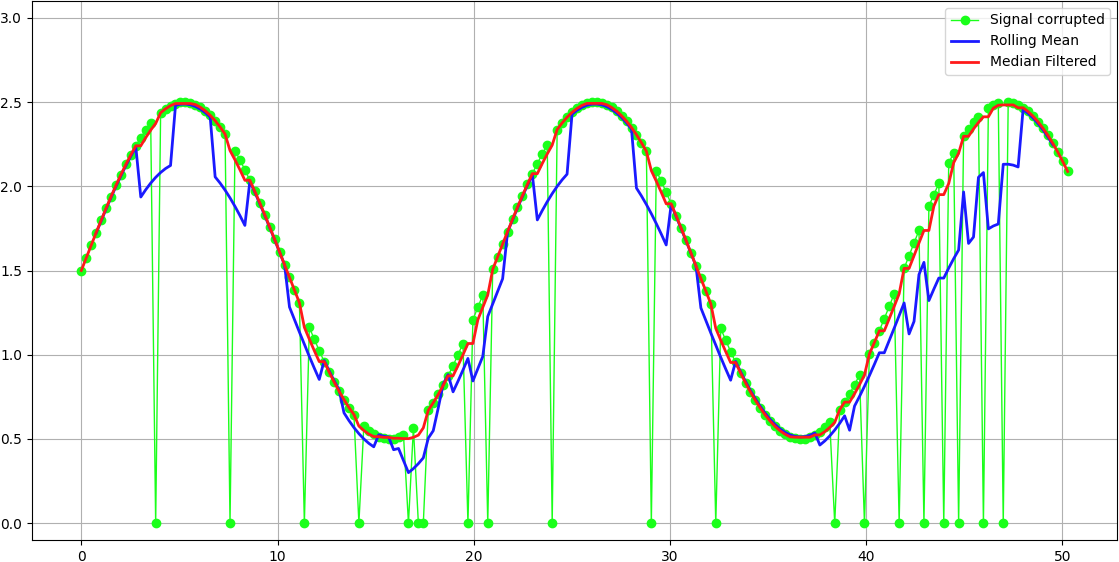
\includegraphics[width=\linewidth]{sin_corrupted_smoothed.png}
    \caption{A sinusoidal signal with corrupted data and smoothing methods applied}
    \label{fig:sin_corrupted_smooted}
\end{figure}


\section{Graph theory}
This section contains definitions, notation and concepts related to Graph Theory according
to \cite{graph_theory:2010}.
Graph theory deals with connection amongst vertices by edges.
Graphs are the foundation of many day to day processes and concepts, as they provide a convenient
and intuitive way of representing objects.

\subsection{Simple graphs}
A \textbf{simple graph} \textit{G} consists of a non-empty finite set \textit{V(G)} of elements called \textbf{vertices}
(or \textbf{nodes}), and a finite set \textit{E(G)} of distinct unordered pairs of distinct elements of \textit{V(G)}
called \textbf{edges}. We call \textit{V(G)} the \textbf{vertices set} and \textit{E(G)} the \textbf{edge set} of G.
An edge $\{\textit{v}, \textit{w}\}$ is said to join the vertices v and w, and is usually abbreviated to vw. For example, Figure~\ref{fig:simple_graph} represents the simple graph G whose vertex set \textit{V(G)} is $\{\textit{u}, \textit{v}, \textit{w}, \textit{z}\}$, and whose
edge set \textit{E(G)} consists of the edges \textit{uv}, \textit{uw}, \textit{vw} and \textit{wz}. 

\begin{figure}[H]
    \centering
    \begin{tikzpicture}
      % Disegno dei nodi
      \node[circle, draw, minimum size=0.7cm] (v) at (0,0) {v};
      \node[circle, draw, minimum size=0.7cm] (u) at (2,0) {u};
      \node[circle, draw, minimum size=0.7cm] (w) at (2,-2) {w};
      \node[circle, draw, minimum size=0.7cm] (z) at (0,-2) {z};
      
      % Disegno degli archi
      \draw (u) -- (v);
      \draw (u) -- (w);
      \draw (v) -- (w);
      \draw (w) -- (z);
    \end{tikzpicture}
    \caption{A simple graph}
    \label{fig:simple_graph}
\end{figure}

\subsection{Adjacency}
We say that two vertices \textit{v} and \textit{w} of a graph \textit{G} are \textbf{adjacent} if there is an edge \textit{vw} joining them, and the vertices \textit{v} and \textit{w} are then \textbf{incident} with such an edge. \\
Similarly, two distinct edges \textit{e} and \textit{f} are \textbf{adjacent} if they have a vertex in common (see Figure \ref{fig:adiacency}).

\begin{figure}[H]
    \centering
    \begin{tikzpicture}
      % Primo grafo
      \node[circle, draw, minimum size=0.7cm] (v) at (0,0) {v};
      \node[circle, draw, minimum size=0.7cm] (w) at (2,0) {w};
      \draw (v) -- (w);
    \end{tikzpicture}
    \quad % Spazio tra i grafi
    \begin{tikzpicture}
      % Secondo grafo
      \node[circle, draw, minimum size=0.7cm] (a) at (0,0) {a};
      \node[circle, draw, minimum size=0.7cm] (b) at (2,1) {b};
      \node[circle, draw, minimum size=0.7cm] (c) at (2,-1) {c};
      \draw (a) -- node[above] {e} (b);
      \draw (a) -- node[below] {f} (c);
    \end{tikzpicture}
    \caption{Adjacent vertices and adjacent edges}
    \label{fig:adiacency}
\end{figure}

\subsection{Weighted Degree Centrality}
\label{subsec:weighted_degree}
Weighted degree centrality is a measure used in network analysis to quantify the importance or centrality of a node in a network, taking into account the weights of the edges connected to that node. 
Unlike traditional degree centrality, which only considers the number of connections (edges) a node has, weighted degree centrality considers the strengths or weights associated with those connections.
For a given node, calculate its weighted degree by summing up the weights of all the edges connected to that node. In mathematical terms, it can be expressed as:
\begin{equation}
  WDC(v) = \sum_{i=1}^{N} w_{vi}
\end{equation}
Where \textit{v} is a vertex in the graph and \textit{N} is the number of vertices.

\subsection{Matrix representations}
One approach to representing a graph is through the use of matrices, especially when dealing with large graphs that may not be well-suited for diagram-based representations.\\
Let's consider a graph \textit{G} with \textit{n} vertices and \textit{m} edges. \\
An \textbf{adjacency matrix A} is the $n \times n$ matrix whose \textit{ij}-th entry is the number of edges joining vertex \textit{i} and vertex \textit{j}. \\
If, in addition, the edges are labelled $\{1, 2, \dots, m\}$, its \textbf{incidence matrix M} is the $n \times m$ matrix whose \textit{ij}-th entry is 1 if vertex \textit{i} is incident to edge \textit{j}, and 0 otherwise. \\
An example of this is given in Figure \ref{fig:matrix_representations}.

\begin{figure}[H]
    \centering
    \begin{minipage}{0.5\textwidth}
        \centering
        \begin{tikzpicture}
            % Nodi
            \node[circle, draw, minimum size=0.7cm] (a) at (0,0) {a};
            \node[circle, draw, minimum size=0.7cm] (b) at (2,2) {b};
            \node[circle, draw, minimum size=0.7cm] (c) at (4,0) {c};
            \node[circle, draw, minimum size=0.7cm] (d) at (2,-2) {d};
          
            % Archi
            \draw (a) edge node[pos=0.5, below] {4} (d);
            \draw (a) edge node[pos=0.5, above] {1} (b);
            \draw (b) edge[bend left] node[pos=0.5, right] {5} (d);
            \draw (b) edge[bend right] node[pos=0.5, left] {6} (d);
            \draw (b) edge node[pos=0.5, above] {2} (c);
            \draw (c) edge node[pos=0.5, below] {3} (d);
        \end{tikzpicture}
    \end{minipage}%
    \begin{minipage}{0.5\textwidth}
        \[
        A = \begin{bmatrix}
        0 & 1 & 0 & 1 \\
        1 & 0 & 1 & 2 \\
        0 & 1 & 0 & 1 \\
        1 & 2 & 1 & 0
        \end{bmatrix}
        \]
        
        \[
        M = \begin{bmatrix}
        1 & 0 & 0 & 1 & 0 & 0 \\
        1 & 1 & 0 & 0 & 1 & 1 \\
        0 & 1 & 1 & 0 & 0 & 0 \\
        0 & 0 & 1 & 1 & 1 & 1
        \end{bmatrix}
        \]
    \end{minipage}
    \caption{Graph \textit{G} with its adjacency \textit{A} and incidence \textit{M} matrices}
    \label{fig:matrix_representations}
\end{figure}


\subsection{Bipartite graphs}
If the vertex set of a graph \textit{G} can be split into two disjoint sets \textit{A} and \textit{B} so that each
edge of \textit{G} joins a vertex of \textit{A} and a vertex of \textit{b}, then \textit{G} is a \textbf{bipartite graph}. \\
Alternatively, a bipartite graph is one whose vertices can be coloured red and blue in such a way that each edge joins a red vertex (in \textit{A}) and a blue vertex (in \textit{B}). \\

\begin{figure}[H]
    \centering
    \begin{tikzpicture}[every node/.style={circle, draw, minimum size=0.7cm}]
        % Livello superiore
        \node (A) at (3,0) [fill=red!75] {a};
        \node (B) at (3,-3) [fill=red!75] {b};
        
        % Livello inferiore
        \node (C) at (5,0) [fill=blue!75] {c};
        \node (D) at (5,-1.5) [fill=blue!75] {d};
        \node (E) at (5,-3) [fill=blue!75] {e};
        
        % Collegamenti
        \draw (A) -- (C);
        \draw (A) -- (E);
        \draw (B) -- (D);
        \draw (B) -- (E);
    \end{tikzpicture}
    \caption{A simple bipartite graph}
    \label{fig:bipartite}
\end{figure}



\subsection{Bipartite graphs with matching}
A \textbf{bipartite graph with matching} is a bipartite graph in which there is a set of edges selected in such a way that no node is shared among the edges of the matching.
In other words, each node is involved in at most one edge of the matching. \\
This means that if the number of vertices in \textit{A} and \textit{B} is different, at least one vertex will have no connection to another vertex (see Figure \ref{fig:match_1}). \\
If there is the same number of vertices in both \textit{A} and \textit{B}, every vertex is connected to another vertex (see Figure \ref{fig:match_2}). \\

\begin{figure}[H]
  \centering
  \begin{subfigure}{0.48\linewidth}
    \centering
    \begin{tikzpicture}[every node/.style={circle, draw, minimum size=0.7cm}]
      % Livello superiore
      \node (A) at (3,0) [fill=red!75] {a};
      \node (B) at (3,-3) [fill=red!75] {b};

      % Livello inferiore
      \node (C) at (5,0) [fill=blue!75] {c};
      \node (D) at (5,-1.5) [fill=blue!75] {d};
      \node (E) at (5,-3) [fill=blue!75] {e};

      % Collegamenti
      \draw (A) -- (C);
      \draw (B) -- (D);
    \end{tikzpicture}
    \caption{}
    \label{fig:match_1}
  \end{subfigure}
  \hspace{0.02\linewidth}
  \begin{subfigure}{0.48\linewidth}
    \centering
    \begin{tikzpicture}[every node/.style={circle, draw, minimum size=0.7cm}]
      % Livello superiore
      \node (A) at (3,0) [fill=red!75] {a};
      \node (B) at (3,-1.5) [fill=red!75] {b};
      \node (C) at (3,-3) [fill=red!75] {c};

      % Livello inferiore
      \node (D) at (5,0) [fill=blue!75] {d};
      \node (E) at (5,-1.5) [fill=blue!75] {e};
      \node (F) at (5,-3) [fill=blue!75] {f};

      % Collegamenti
      \draw (A) -- (E);
      \draw (B) -- (F);
      \draw (C) -- (D);
    \end{tikzpicture}
    \caption{}
    \label{fig:match_2}
  \end{subfigure}
  \caption{Bipartite graph}
\end{figure}

\subsection{Maximum Weight Perfect Matching}
\label{sec:MaxWPM}
The Maximum Perfect Weight Matching is an optimization problem concerning graphs.
The graphs in question are bipartite, meaning the vertices can be divided into two distinct sets in such a way that all edges of the graph connect vertices from different sets, with no edges connecting vertices within the same set.
Additionally, these graphs are undirected, meaning the relationship between two nodes is bidirectional, in other words, the edge connecting node A to node B automatically implies the existence of the edge connecting node B to node A. \\
In the MaxWPM problem, the vertices represent elements to be paired, and the edges represent possible connections between these elements. 
Each edge is associated with a weight that represents the value or importance of the pairing between the connected vertices.\\
The goal is to find a perfect matching, which is a set of edges in which every node is connected to exactly one other node, with no overlaps or isolated nodes, while maximizing the total weight of the edges in the matching.
The total weight is the sum of the weights of the edges included in the matching.
The weights of the edges are collected in a matrix called a \textit{utility matrix}.\\
The utility matrix will be a square matrix because the number of nodes in the two distinct sets is the same.
The rows could represent the nodes in the first set, while the columns could represent the nodes in the second set, or vice versa.
The element (\textit{i}, \textit{j}) of the matrix represents the weight of the edge connecting vertex \textit{i} to vertex \textit{j}.

A MaxWPM problem using an utility matrix can be transformed into a \textbf{Minimum Weight Perfect Matching} problem.
This can be achieved by introducing an auxiliary matrix, referred to as the \textit{cost matrix}.
The cost matrix is essentially a duplicate of the utility matrix, but with all its elements negated.

\subsection{Brute Force Algorithm}
\label{sec:bf}
The BF can be a possible approach to solve the MaxWPM problem for bipartite graphs.
However, it is important to note that the BF has exponential time complexity, specifically, its time complexity grows exponentially with the number of vertices in the graph.
This is because the BF examines all possible combinations of matchings within the bipartite graph to find the one with the maximum weight.\\
If the graph has \textit{n} vertices in both the first and second partitions, there are \textit{n}!\ possible matchings.
Each matching requires \textit{O}(\textit{n}) time to be computed because you need to check that it is a perfect matching and calculate its total weight.
Therefore, the overall complexity of the algorithm is on the order of \textit{O}(\textit{n}!$\cdot$\textit{n}).
Since the complexity grows rapidly as \textit{n} increases, it quickly becomes impractical for large-sized graphs. \\
The operation of the BF for MinWPM problems can be summerized in these 3 steps:
\begin{enumerate}
    \item {Compute the cost matrix for the considered bipartite graph with \textit{n} vertices in each partition.}
    \item {Compute the total cost of all the \textit{n}!\ permutations.}
    \item {Choose the assignment with the lowest total cost.}
\end{enumerate}


\subsection{Hungarian Matching Algorithm}
\label{sec:ha}

The HM, also called the Kuhn-Munkres algorithm, is a \textit{O}($\textit{n}^3$) algorithm that can be used to find MaxWPM in bipartite graphs with \textit{n} vertices for each partition, which is sometimes called the assignment problem.
As previously demonstrated in the Brute Force algorithm, maximum-weight perfect matching problems using the utility matrix can be converted into MinWPM problems using the cost matrix. 
We will describe the application of the HM to address Minimum Weight Perfect Matching problems.\\
The operation of the HM for MinWPM problems can be summerized in these 6 steps:
\begin{enumerate}
    \item {Compute the cost matrix for the considered bipartite graph with \textit{n} vertices in each partition.}
    \item {Subtract the smallest entry in each row from all the other entries in the row. This will make the smallest entry in the row now equal to 0.}
    \item {Subtract the smallest entry in each column from all the other entries in the column. This will make the smallest entry in the column now equal to 0.}
    \item {Draw lines through the row and columns that have the 0 entries such that the fewest lines possible are drawn.}
    \item {If there are n lines drawn, an optimal assignment of zeros is possible and the algorithm is finished. If the number of lines is less than n, then the optimal number of zeroes is not yet reached. Go to the next step.}
    \item {Find the smallest entry not covered by any line. Subtract this entry from each row that isn’t crossed out, and then add it to each column that is crossed out. Then, go back to Step 3.}
\end{enumerate}
Let's take an example of a cost matrix and try to apply the HM for MinWPM problems as in Table \ref{tab:hung_alg}:

\begin{enumerate}
  \item[(a)] From the original table that describes the cost associated for every assignment
  \item[(b)] Subtract the smallest value in each row from the other values in the row
  \item[(c)] Now, subtract the smallest value in each column from all other values in the column
  \item[(d)] Since there are 2 lines drawn, less than 3, so there is not yet the optimal number of zeroes. 
  \item[(e)] Find the smallest entry not covered by any line. Subtract this entry from each row that isn’t crossed out, and then add it to each column that is crossed out. 
              Then, go back to step (c). 2 is the smallest entry. First, subtract from the uncovered rows.
  \item[(f)] Now add to the covered columns
  \item[(g)] Now go back to step (c), drawing lines through the rows and columns that have 0 entries 
  \item[(h)] There are 3 lines, so we are done. The assignment will be where the 0's are in the matrix such that only one 0 per row and column is part of the assignment.
  \item[(i)] And this results in the following minimum total cost for the assignment problem. 
\end{enumerate}

\begin{table}[H]
  \centering
  \begin{minipage}{0.3\textwidth}
    \centering
    \begin{tabular}{|>{\centering\arraybackslash}m{0.6cm}|>{\centering\arraybackslash}m{0.6cm}|>{\centering\arraybackslash}m{0.6cm}|}
      \hline
      108 & 125 & 150 \\
      \hline
      150 & 135 & 175 \\
      \hline
      122 & 148 & 250 \\
      \hline
    \end{tabular}
    \caption*{(a)}
  \end{minipage}
  \hfill
  \begin{minipage}{0.3\textwidth}
    \centering
    \begin{tabular}{|>{\centering\arraybackslash}m{0.6cm}|>{\centering\arraybackslash}m{0.6cm}|>{\centering\arraybackslash}m{0.6cm}|}
      \hline
      0 & 17 & 42 \\
      \hline
      15 & 0 & 40 \\
      \hline
      0 & 26 & 128 \\
      \hline
    \end{tabular}
    \caption*{(b)}
  \end{minipage}
  \hfill
  \begin{minipage}{0.3\textwidth}
    \centering
    \begin{tabular}{|>{\centering\arraybackslash}m{0.6cm}|>{\centering\arraybackslash}m{0.6cm}|>{\centering\arraybackslash}m{0.6cm}|}
      \hline
      0 & 17 & 2 \\
      \hline
      15 & 0 & 0 \\
      \hline
      0 & 26 & 88 \\
      \hline
    \end{tabular}
    \caption*{(c)}
  \end{minipage}

  \vspace{10pt}

  \begin{minipage}{0.3\textwidth}
    \centering
    \begin{tabular}{|>{\centering\arraybackslash}m{0.6cm}|>{\centering\arraybackslash}m{0.6cm}|>{\centering\arraybackslash}m{0.6cm}|}
      \hline
      \cellcolor{gray!25} 0 & 17 & 2 \\
      \hline
      \cellcolor{gray!25} 15 & \cellcolor{gray!25} 0 & \cellcolor{gray!25} 0 \\
      \hline
      \cellcolor{gray!25} 0 & 26 & 88 \\
      \hline
    \end{tabular}
    \caption*{(d)}
  \end{minipage}
  \hfill
  \begin{minipage}{0.3\textwidth}
    \centering
    \begin{tabular}{|>{\centering\arraybackslash}m{0.6cm}|>{\centering\arraybackslash}m{0.6cm}|>{\centering\arraybackslash}m{0.6cm}|}
      \hline
      \cellcolor{gray!25} -2 & 15 & 0 \\
      \hline
      \cellcolor{gray!25} 15 & \cellcolor{gray!25} 0 & \cellcolor{gray!25} 0 \\
      \hline
      \cellcolor{gray!25} -2 & 24 & 86 \\
      \hline
    \end{tabular}
    \caption*{(e)}
  \end{minipage}
  \hfill
  \begin{minipage}{0.3\textwidth}
    \centering
    \begin{tabular}{|>{\centering\arraybackslash}m{0.6cm}|>{\centering\arraybackslash}m{0.6cm}|>{\centering\arraybackslash}m{0.6cm}|}
      \hline
      \cellcolor{gray!25} 0 & 15 & 0 \\
      \hline
      \cellcolor{gray!25} 17 & \cellcolor{gray!25} 0 & \cellcolor{gray!25} 0 \\
      \hline
      \cellcolor{gray!25} 0 & 24 & 86 \\
      \hline
    \end{tabular}
    \caption*{(f)}
  \end{minipage}

  \vspace{10pt}

  \begin{minipage}{0.3\textwidth}
    \centering
    \begin{tabular}{|>{\centering\arraybackslash}m{0.6cm}|>{\centering\arraybackslash}m{0.6cm}|>{\centering\arraybackslash}m{0.6cm}|}
      \hline
      \cellcolor{gray!25} 0 & \cellcolor{gray!25} 15 & \cellcolor{gray!25} 0 \\
      \hline
      \cellcolor{gray!25} 17 & \cellcolor{gray!25} 0 & \cellcolor{gray!25} 0 \\
      \hline
      \cellcolor{gray!25} 0 & 24 & 86 \\
      \hline
    \end{tabular}
    \caption*{(g)}
  \end{minipage}
  \hfill
  \begin{minipage}{0.3\textwidth}
    \centering
    \begin{tabular}{|>{\centering\arraybackslash}m{0.6cm}|>{\centering\arraybackslash}m{0.6cm}|>{\centering\arraybackslash}m{0.6cm}|}
      \hline
      0 & 15 & \cellcolor{green!75} 0 \\
      \hline
      17 & \cellcolor{green!75} 0 & 0 \\
      \hline
      \cellcolor{green!75} 0 & 24 & 86 \\
      \hline
    \end{tabular}
    \caption*{(h)}
  \end{minipage}
  \hfill
  \begin{minipage}{0.3\textwidth}
    \centering
    \begin{tabular}{|>{\centering\arraybackslash}m{0.6cm}|>{\centering\arraybackslash}m{0.6cm}|>{\centering\arraybackslash}m{0.6cm}|}
      \hline
      108 & 125 & \cellcolor{green!75} 150 \\
      \hline
      150 & \cellcolor{green!75} 135 & 175 \\
      \hline
      \cellcolor{green!75} 122 & 148 & 250 \\
      \hline
    \end{tabular}
    \caption*{(i)}
  \end{minipage}
  \caption{Resolution of the Hungarian Algorithm}
  \label{tab:hung_alg}
\end{table}

\subsection{Cosine Similarity}
\label{subsec:cosine_sim}
Cosine similarity is a measure of similarity between two vectors, frequently used to gauge how aligned vectors are in space. \\ 
It returns a value ranging from -1 to 1. 
The concept is that similar vectors will have a small angle between them, resulting in a cosine similarity value close to 1. \\ 
Conversely, dissimilar vectors will have a wide angle and a cosine similarity close to 0.\\ 
A higher value indicates greater similarity, where 1 represents identical vectors (perfect similarity), 0 means no similarity, and -1 indicates perfect dissimilarity (opposite directions). 
We iteratively calculate the similarity between all the joints connected by an edge. 
The cosine similarity between two vectors \textit{x} and \textit{y} is defined as: 

\begin{equation}  
  cos(\vec{x}, \vec{y}) = \frac{\vec{x} \cdot \vec{y}}{\|\vec{x}\| \cdot \|\vec{y}\|}  =  \frac{\sum_{i=1}^{3} (x_i \cdot y_i)}{\sqrt{\sum_{i=1}^{3} x_i^2} \cdot \sqrt{\sum_{i=1}^{3} y_i^2}}    
\end{equation} 



\section{Machine Learning Theory}
\label{subsec:ML}

ML deals with the ability of a system to improve its performance through experience, without being explicitly programmed.
It also serves as the foundation for numerous everyday applications and concepts, 
as it provides a powerful and efficient way to address complex challenges, make data-driven decisions, 
and develop intelligent systems that can learn and adapt autonomously.\\
Diving deeper into this concept, one critical aspect is the role of hyperparameters. 
Hyperparameters are settings or configurations that guide the learning process of ML algorithms. 
They act as the levers that fine-tune the behavior of these algorithms, influencing their performance, accuracy, and generalization capabilities.\\
Hyperparameters encompass a wide range of choices, such as the learning rate in gradient descent, the depth of a decision tree, the number of hidden layers in a neural network, or the number of clusters in a k-means clustering algorithm. 
Selecting the right hyperparameters can be a challenging and often iterative task, as they significantly impact the model's ability to capture underlying patterns in data.\\
The process of hyperparameter tuning involves experimenting with different combinations of values, assessing the model's performance using techniques like cross-validation, and iteratively adjusting the hyperparameters to optimize the model's accuracy and generalization. 
This fine-tuning is crucial to ensure that the ML model not only fits the training data well but also performs effectively on unseen data.
Moreover, the choice of hyperparameters is problem-dependent, and there's no one-size-fits-all solution. 
It requires a deep understanding of the algorithm, the dataset, and the specific problem at hand.

\subsection{Classifier}
\label{subsec:classifier}

A mathematical \textbf{Classifier} is a model that takes an input dataset and assigns each data point to a class or category. 
The mathematical formulation of a classifier can vary depending on the algorithm used. 
Suppose we have a training dataset represented as pairs (\textit{$\overline{x}$}, \textit{y}), where \textit{$\overline{x}$} is a vector of data features, and \textit{y} is the associated class label.
The \textit{y} is a categorical (can take a fixed, number of possible values) variable that categorizes between two or more classes (e.g.: dog, cat, bird), while in a regression problem it is a continuous variable.
Our goal is to find a function \textit{f}(\textit{$\overline{x}$}) that maps the feature vectors \textit{$\overline{x}$} to class labels \textit{y}. \\

A \textbf{Binary Classification Problem} is a specific type of classification problem where the goal is to categorize input data into one of two distinct classes or categories. 
These two classes are typically referred to as the positive class and the negative class, and the task is to assign each data point to one of these two classes based on its features or attributes.
\begin{figure}[H]
  \centering
  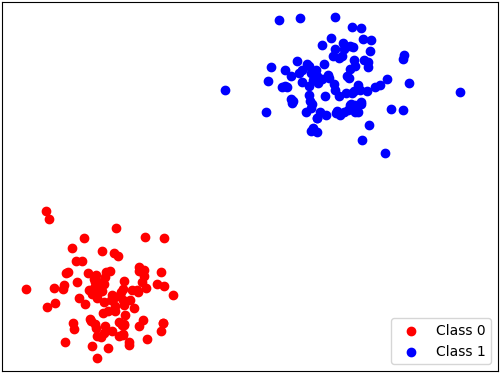
\includegraphics[width=0.55\linewidth]{BinaryClassification.png}
  \caption{A binary classification example}
  \label{fig:bin_classification}
\end{figure}

\subsection{K-Nearest Neighbors}
\label{subsec:KNN}

The \textbf{KNN} algorithm is a supervised ML algorithm used for classification and regression tasks.
It is a simple and intuitive algorithm that makes predictions based on the similarity between a data point and its \textit{k}-nearest neighbors in a training dataset.
The \textit{k} in \textit{k}-nearest neighbors refers to the number of items that the algorithm uses to make its prediction whether its a classification problem or a regression problem.
In Figure \ref{fig:knn} we can see a test sample represented by a green dot and we want to classify 
it either as a blue square or a red triangle based on a KNN algorithm, the decision depends on the value of \textit{k}, which determines how many nearest neighbors we consider.\\
When \textit{k} = 3 (solid line circle), the green dot is assigned to the category that has the majority among its three nearest neighbors. 
In this case, if there are 2 red triangles and only 1 blue square inside the inner circle, the green dot is classified as a red triangle. \\
When \textit{k} = 5 (dashed line circle), the green dot is assigned to the category with the majority among its five nearest neighbors. 
If there are 3 blue squares and 2 red triangles inside the outer circle, the green dot is classified as a blue square.
\begin{figure}[H]
    \centering
    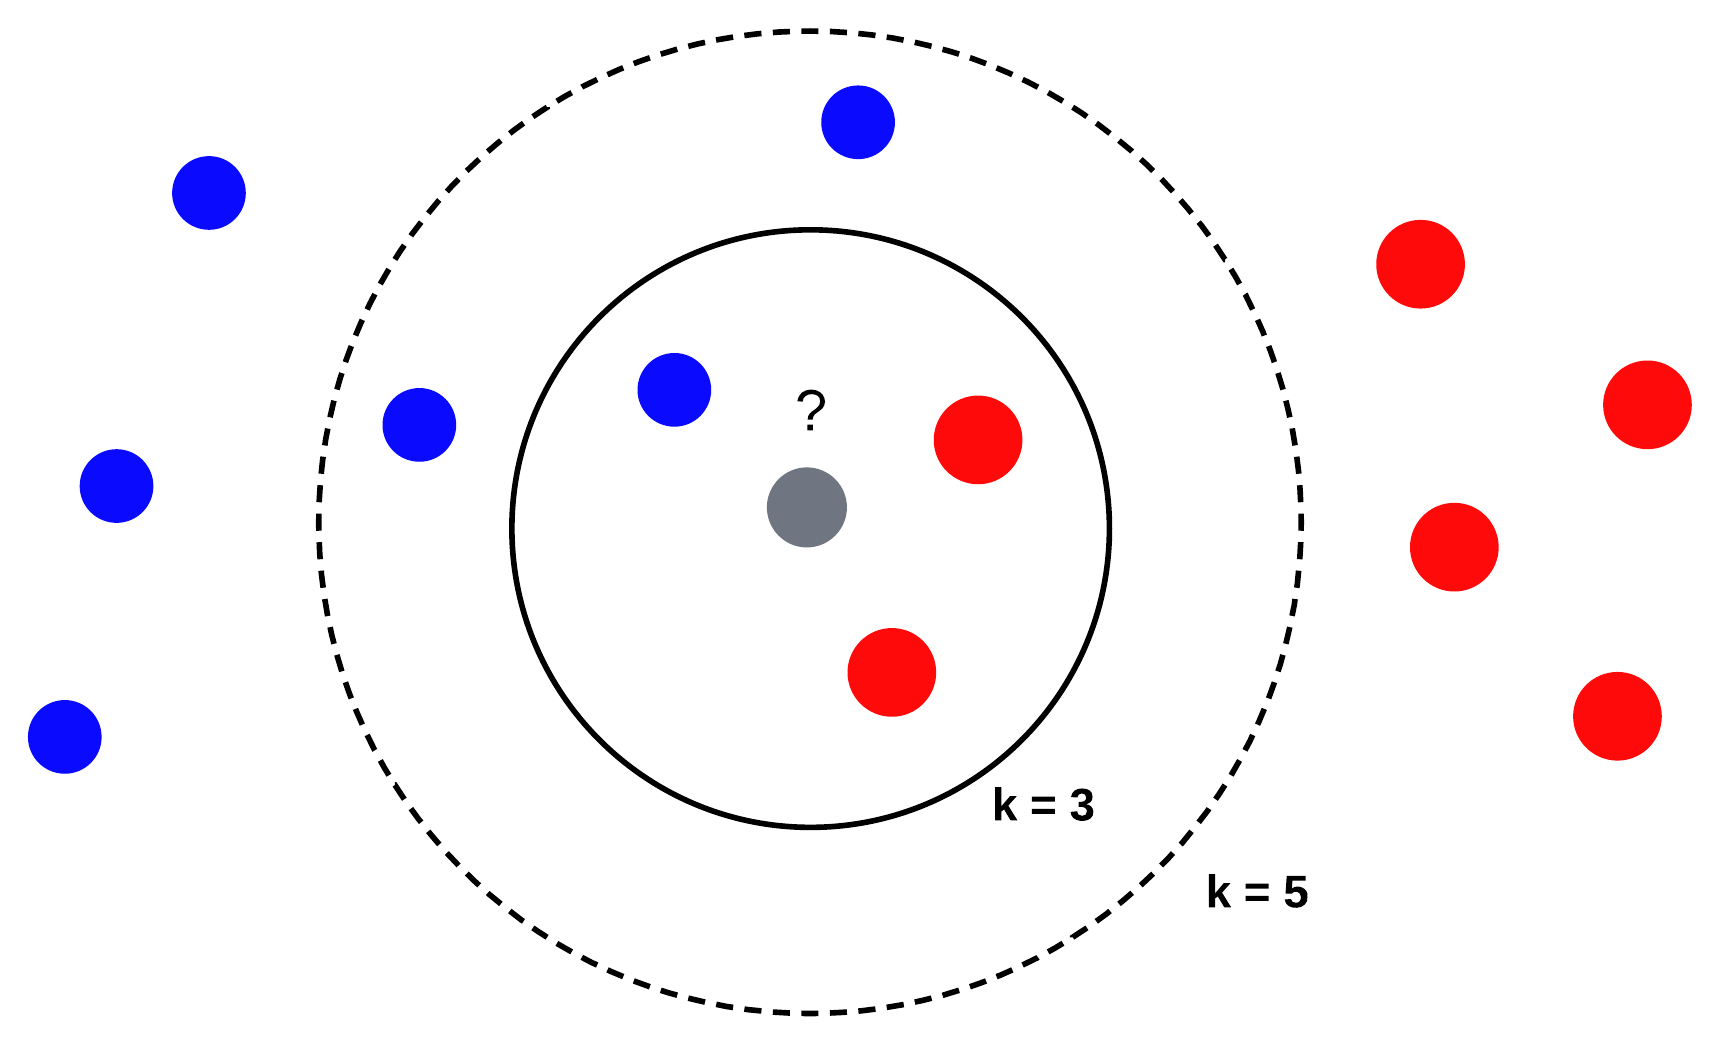
\includegraphics[width=0.7\linewidth]{KNeighbours.png}
    \caption{KNN algorithm with \textit{k} = 3 and \textit{k} = 5}
    \label{fig:knn}
\end{figure}

The choice of distance metric is a critical aspect of the KNN algorithm, and while it is not typically considered a hyperparameter, it significantly influences the model's performance and outcomes. 
The selection of a specific distance metric can have a substantial impact, especially when dealing with datasets of varying sizes and dimensions. \\
If we consider for example two data points \textit{p}, \textit{q} in \textit{n}-dimensional space, there are various distance metrics that can be used to find the neighbors.\\
Among the different  most common is the Euclidean distance: 
\begin{equation}
    Euclidean(p,q) = \sqrt{\sum_{i=1}^{n} (p_i - q_i)^2}
    \label{formula:distance}
\end{equation}

\subsection{Borderline Synthetic Minority Over-sampling Technique}
\label{subsec:borderline}

\textbf{Oversampling} is a technique used in the field of imbalanced ML to address the problem of class imbalance. 
Class imbalance occurs when one class in a classification problem has significantly fewer instances than another class. 
This imbalance can lead to biased models that perform poorly on the minority class (the class with fewer instances) because the model tends to be biased towards the majority class.\\
The concept of oversampling involves increasing the number of instances in the minority class by generating synthetic or duplicate samples. 
The goal is to balance the class distribution, making the minority class more comparable in size to the majority class. 
A synthetic sample can be generated duplicating randomly another sample of the minority class or considering its underlying data distribution (ADASYN \cite{adasyn:2008}).
This could result in a performance improvement of ML models by providing them with more information about the minority class.\\
The SMOTE generates synthetic samples by interpolating between neighboring minority class instances using an underlying KNN model.\\

The \textbf{B-SMOTE} \cite{Han2005BorderlineSMOTEAN:2005}, is a vairant of the SMOTE that focuses on generating synthetic samples only for the boundary instances, which are the minority class instances close to the majority class. 
This approach aims to concentrate on the regions of the dataset that are near the decision boundary between classes. \\
The model internally fits two instances of KNN with different parameters \textit{k-neighbors} and \textit{m-neighbors}: one instance defines the neighborhood of samples to generate the synthetic samples; the other, instead, is used to determine if a minority sample is in \textit{danger}.\\
A \textit{sample in danger} is one near to the boundary between two or more classes.

In the illustrated scenario depicted in Figure \ref{fig:bordSMOTEnotApplied}, the task involves categorizing two distinct categories of network traffic: 
one being malicious (depicted in red), the other representing legitimate traffic (shown in blue), and the decision boundaries are the same color meshes.
The distribution of malicious traffic is more sparse and rare compared to legitimate traffic, this means that the classifier has been trained on an imbalanced dataset. 
The primary objective of the classification is to maximize the detection of malicious traffic, even if it entails misclassifying some instances of legitimate traffic. 
B-SMOTE is a possible solution for this scenario, where the two classes are significantly imbalanced, and the weight of legitimate traffic in the classification process could be overwhelming.

The application of the B-SMOTE algorithm facilitates class rebalancing by generating synthetic data points in the boundary regions between the classes concentrated in proximity of the decision boundary.
In Figure \ref{fig:bordSMOTEApplied}, the depicted image showcases the ultimate outcome achieved following the retraining of the classifier. 
The retraining process maintained the same parameters but employed a dataset that has been more uniformly balanced.
The synthetic samples generated by B-SMOTE are represented as light-red dots.
\begin{figure}[H]
  \centering
  \begin{subfigure}{0.49\linewidth}
    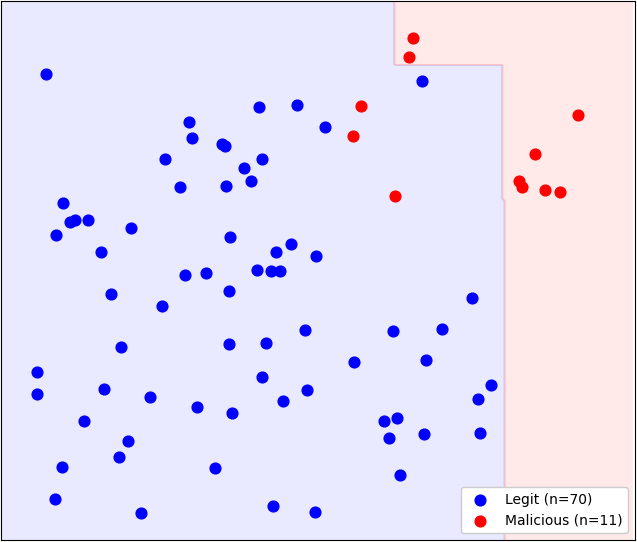
\includegraphics[width=\linewidth]{BordSMOTE_no.png}
    \caption{}
    \label{fig:bordSMOTEnotApplied}
  \end{subfigure}
  %\hspace{0.0\linewidth}
  \begin{subfigure}{0.49\linewidth}
    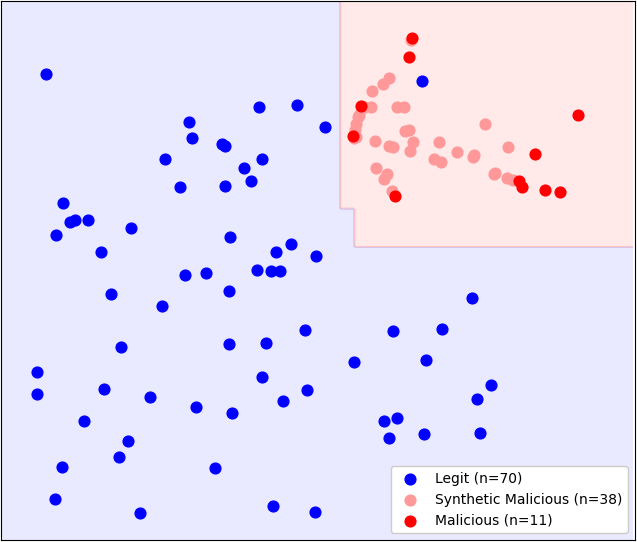
\includegraphics[width=\linewidth]{BordSMOTE_yes.png}
    \caption{}
    \label{fig:bordSMOTEApplied}
  \end{subfigure}
  \caption{Visual representation of B-SMOTE algorithm applied on a dataset}
\end{figure}

However the B-SMOTE algorithm, has its limitations and drawbacks:
\begin{itemize}
  \item \textbf{Risk of Overfitting:} In the provided example, the malicious data was generated using a normal distribution, while the legitimate data was generated using a uniform distribution.
  This means that the second classification fits better the underlying distribution without any a-priori assumption.
  But in some cases depending on the choice of borderline examples, 
  B-SMOTE may introduce a bias towards certain patterns or classes in the synthetic samples, which can affect the model's generalization.
  It can potentially lead to overfitting, especially when it generates a large number of synthetic samples in the borderline region. 
  This may cause the model to perform exceptionally well on the training data but poorly on unseen data.
  \item \textbf{Computationally intensive:} It can require high hardware resources, especially in high-dimensional spaces, as it involves calculating distances between data points. 
  This can lead to longer training times, making it less suitable for large datasets.
  \item \textbf{Designed for Clearly Separable Datasets:} It is designed for datasets with clear class boundaries and is most effective when the borderline instances are well-defined. 
  In cases where class separation is not distinct, it may not provide substantial benefits.
\end{itemize}
So in general, even if it aims to improve the classification of the minority class, there is no guarantee that it will always lead to better results.

\subsection{Random Forest Classifier}
\label{subsec:RF}

A \textbf{Decision Tree} (DT) is a non-parametric supervised learning algorithm, which is utilized for both classification and regression tasks. 
It has a hierarchical, tree structure, which consists of a internal nodes, leaf nodes and branches.
From the root node, splitting criterias are applied on the samples creating branches and child nodes that lead to leaf nodes which represent the final classification of the tree.
The most common impurity measure used to quantify the impurity of a dataset is the Gini criterion:
For a set of items with \textit{J} classes and relative frequencies $p_{i}$, $i \in {1,2,...,J}$ 
the probability of choosing an item with label $i$ is $p_{i}$, and the probability of miscategorizing that item is:
\begin{equation} 
  \sum_{k \ne i} p_{k} = 1 - p_{i} 
\end{equation}
The Gini impurity is computed by summing pairwise products of these probabilities for each class label:
\begin{equation}
  Gini(p) = 1 - \sum_{i=1}^{J} (p_i^2)
\end{equation}

In the example shown in Table \ref{tab:tableDecisionTreeDataset}, the objective is to determine whether to grant a loan based on two pieces of information: 
the applicant's monthly income and the requested loan amount. The second figure illustrates the DT that has been trained on this dataset.
The underlying principle of the DT is that at every non-terminal node, if there exist samples that need further separation, the following algorithm is applied: 
\begin{enumerate}
  \item It starts by calculating the impurity of the current node before making any splits. This initial impurity serves as a baseline for evaluating feature splits.
  \item For each feature in the dataset, calculate a measure of impurity or information gain for potential splits. This typically involves examining the feature values and considering different threshold values.
  \item Calculates the reduction in impurity (or information gain) achieved by the potential split. This is done by comparing the impurity of the current node with the impurity of the child nodes created by the split.
  \item Choose the feature that results in the highest information gain. This feature becomes the one on which to apply the threshold for the split.
  \item It applies the threshold that separates the data into two or more subsets.
  \item Continue the process recursively for each child node created by the split. This means repeating steps 1 to 5 for each child node until a stopping criterion is met (e.g., a maximum tree depth is reached).
\end{enumerate}
The goal is to create child nodes that are as homogeneous as possible with respect to the target variable, thereby improving the predictive accuracy of the tree.
\begin{table}[H]
  \centering
  \begin{tabular}{||>{\centering\arraybackslash}p{3.2cm}||>{\centering\arraybackslash}p{3.2cm}||>{\centering\arraybackslash}p{3.2cm}||}
  \hline
  \textbf{Income} & \textbf{Loan\_Amount} & \textbf{Loan\_Approved} \\
  \hline
  2000 & 300000 & Not Approved \\
  3000 & 300000 & Approved \\
  4000 & 400000 & Not Approved \\
  5000 & 400000 & Not Approved \\
  10000 & 400000 & Approved \\
  15000 & 400000 & Approved \\
  \hline
  \end{tabular}
  \caption{Dataset of the DT}
  \label{tab:tableDecisionTreeDataset}
\end{table}
\begin{figure}[H]
  \centering
  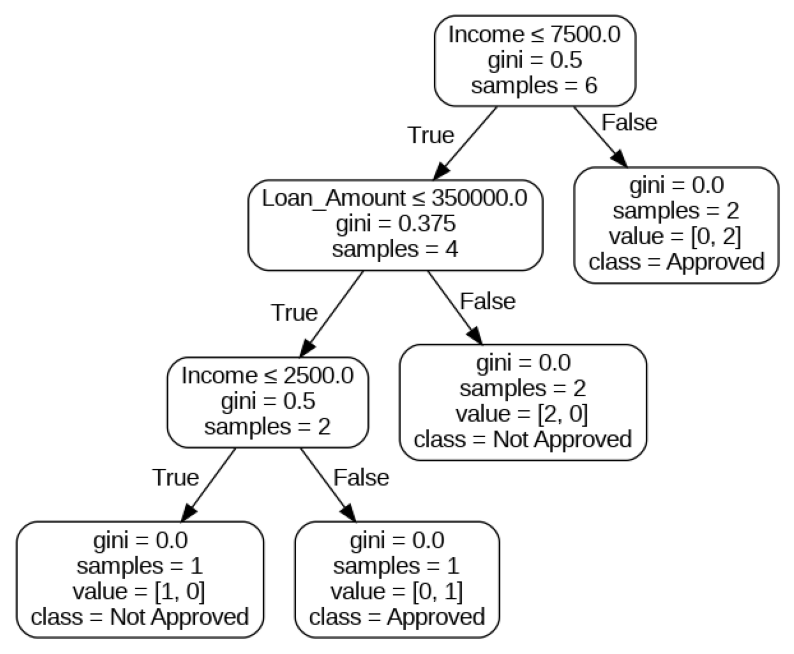
\includegraphics[width=0.6\linewidth]{DecTree.png}
  \label{fig:knn5}
  \caption{DT applied on the dataset of Table \ref{tab:tableDecisionTreeDataset}}
\end{figure}
In the example provided the term “samples" represent the total number of training samples used to create the specific tree node. 
In other words, it is the number of data examples that were considered in that node during the tree construction process.

Note that due to the absence of constraints on hyperparameters like tree depth or the minimum number of features required to split nodes, 
it becomes evident that each sample in the dataset follows a distinct path within this tree. 
The term \textit{value} represents the distribution of classes or labels of the samples within a node. 
It is a vector that indicates how many training samples in that node belong to each class or category. 
For instance, if we see $value$ = [0, 2], it means that there are 0 samples belonging to class \textit{Not Approved} and 2 samples belonging to class \textit{Approved} in that node.
This example is simply used for showing the behaviour of a DT\\
\clearpage
\textbf{Random Forest} is an ensemble learning method that builds multiple DTs during training and combines their predictions to make more accurate and robust classifications or regressions.
A RF is typically constructed in this way:
\begin{enumerate}
  \item \textbf{Bootstrapped Data:} A random subset of the training data (with replacement) is used to train each DT. This results in each tree being trained on a slightly different dataset.
  \item \textbf{Random Feature Selection:} At each node of each DT, only a random subset of the available features is considered for splitting. This helps introduce diversity among the trees and reduces the risk of overfitting.
  \item \textbf{Independent Training:} Each DT is trained independently. There is no communication or shared information between the trees during training.
  \item \textbf{Voting or Averaging:} For classification tasks, the RF combines the individual tree predictions by applying a Majority Voting (each tree votes for a class and the final prediction reflects the class that receives the most votes overall)
\end{enumerate}
The key idea behind the RF method is that by aggregating the predictions of multiple DTs, the ensemble can reduce overfitting, improve generalization, and provide more robust and accurate results.
For example the Figure \ref{fig:rf} is shown a RF classifier made of 3 DTs has been created applying the bootstrap method on the dataset and correctly classifies the first sample of the dataset in Table \ref{tab:tableDecisionTreeDataset}.
\clearpage
\begin{figure}[H]
  \centering
  \begin{subfigure}{0.49\linewidth}
    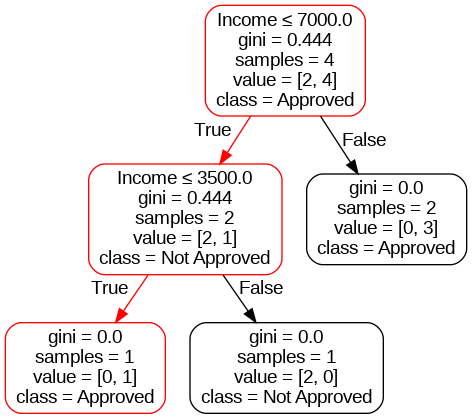
\includegraphics[width=\linewidth]{loan_RF_1.png}
    \caption{}
    \label{fig:rfTree0}
  \end{subfigure}
  %\hspace{0\linewidth}
  \begin{subfigure}{0.49\linewidth}
    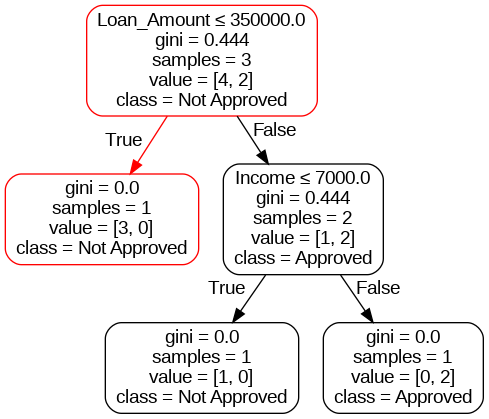
\includegraphics[width=\linewidth]{loan_RF_2.png}
    \caption{}
    \label{fig:rfTree1}
  \end{subfigure}
  \begin{subfigure}{0.4\linewidth}
    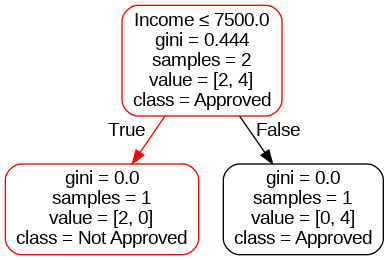
\includegraphics[width=\linewidth]{loan_RF_0.png}
    \caption{}
    \label{fig:rfTree2}
  \end{subfigure}
  \caption{Path taken by the first sample through the three DTs of a RF classifier}
  \label{fig:rf}
\end{figure}


\subsection{Cross Validation}
\label{subsec:cross_validation}

\textbf{Cross Validation} is a technique used to estimate the effectiveness of a ML model based on a data sample.
It involves dividing the dataset into multiple training and testing subsets called \textit{folds} and then training and evaluating the model on each fold.
The process of training and testing is typically repeated multiple times and the results from each iteration are often averaged to provide an overall estimate of the model's performance.
The most common approach in basic cross-validation is to use a 80-20 or 70-30 split between the training and test sets.\\
When we partition our dataset into folds for techniques like cross-validation, it is crucial to ensure that each fold accurately represents the diversity of the entire dataset. 
This entails maintaining the same proportion of different classes or categories within each fold.\\ 
While random splitting is often sufficient, there are instances, particularly in intricate datasets, where we must deliberately enforce the correct distribution of classes within each fold to maintain data integrity.
\\

\textbf{Leave-One-Out Cross-Validation} (LOOCV) is a specific type of cross-validation where the number of folds $k$ is set equal to the number of samples in the dataset $n$. 
In this approach, the model undergoes training k times, with k being precisely the total number of samples $n$.
During each of the \textit{k} iterations, a distinct sample is singled out as the test set, while all the remaining samples are utilized for model training. 
This procedure ensures that every single sample gets its turn as the test set, comprehensively assessing the model's performance across the entire dataset.
In Figure \ref{fig:LOOCV} is shown how it works, note that training and testing is performed on the same model at each iteration.
The evaluation metric is based on the consistency between the predicted values and the actual values across all iterations.

\begin{figure}[H]
  \centering  
    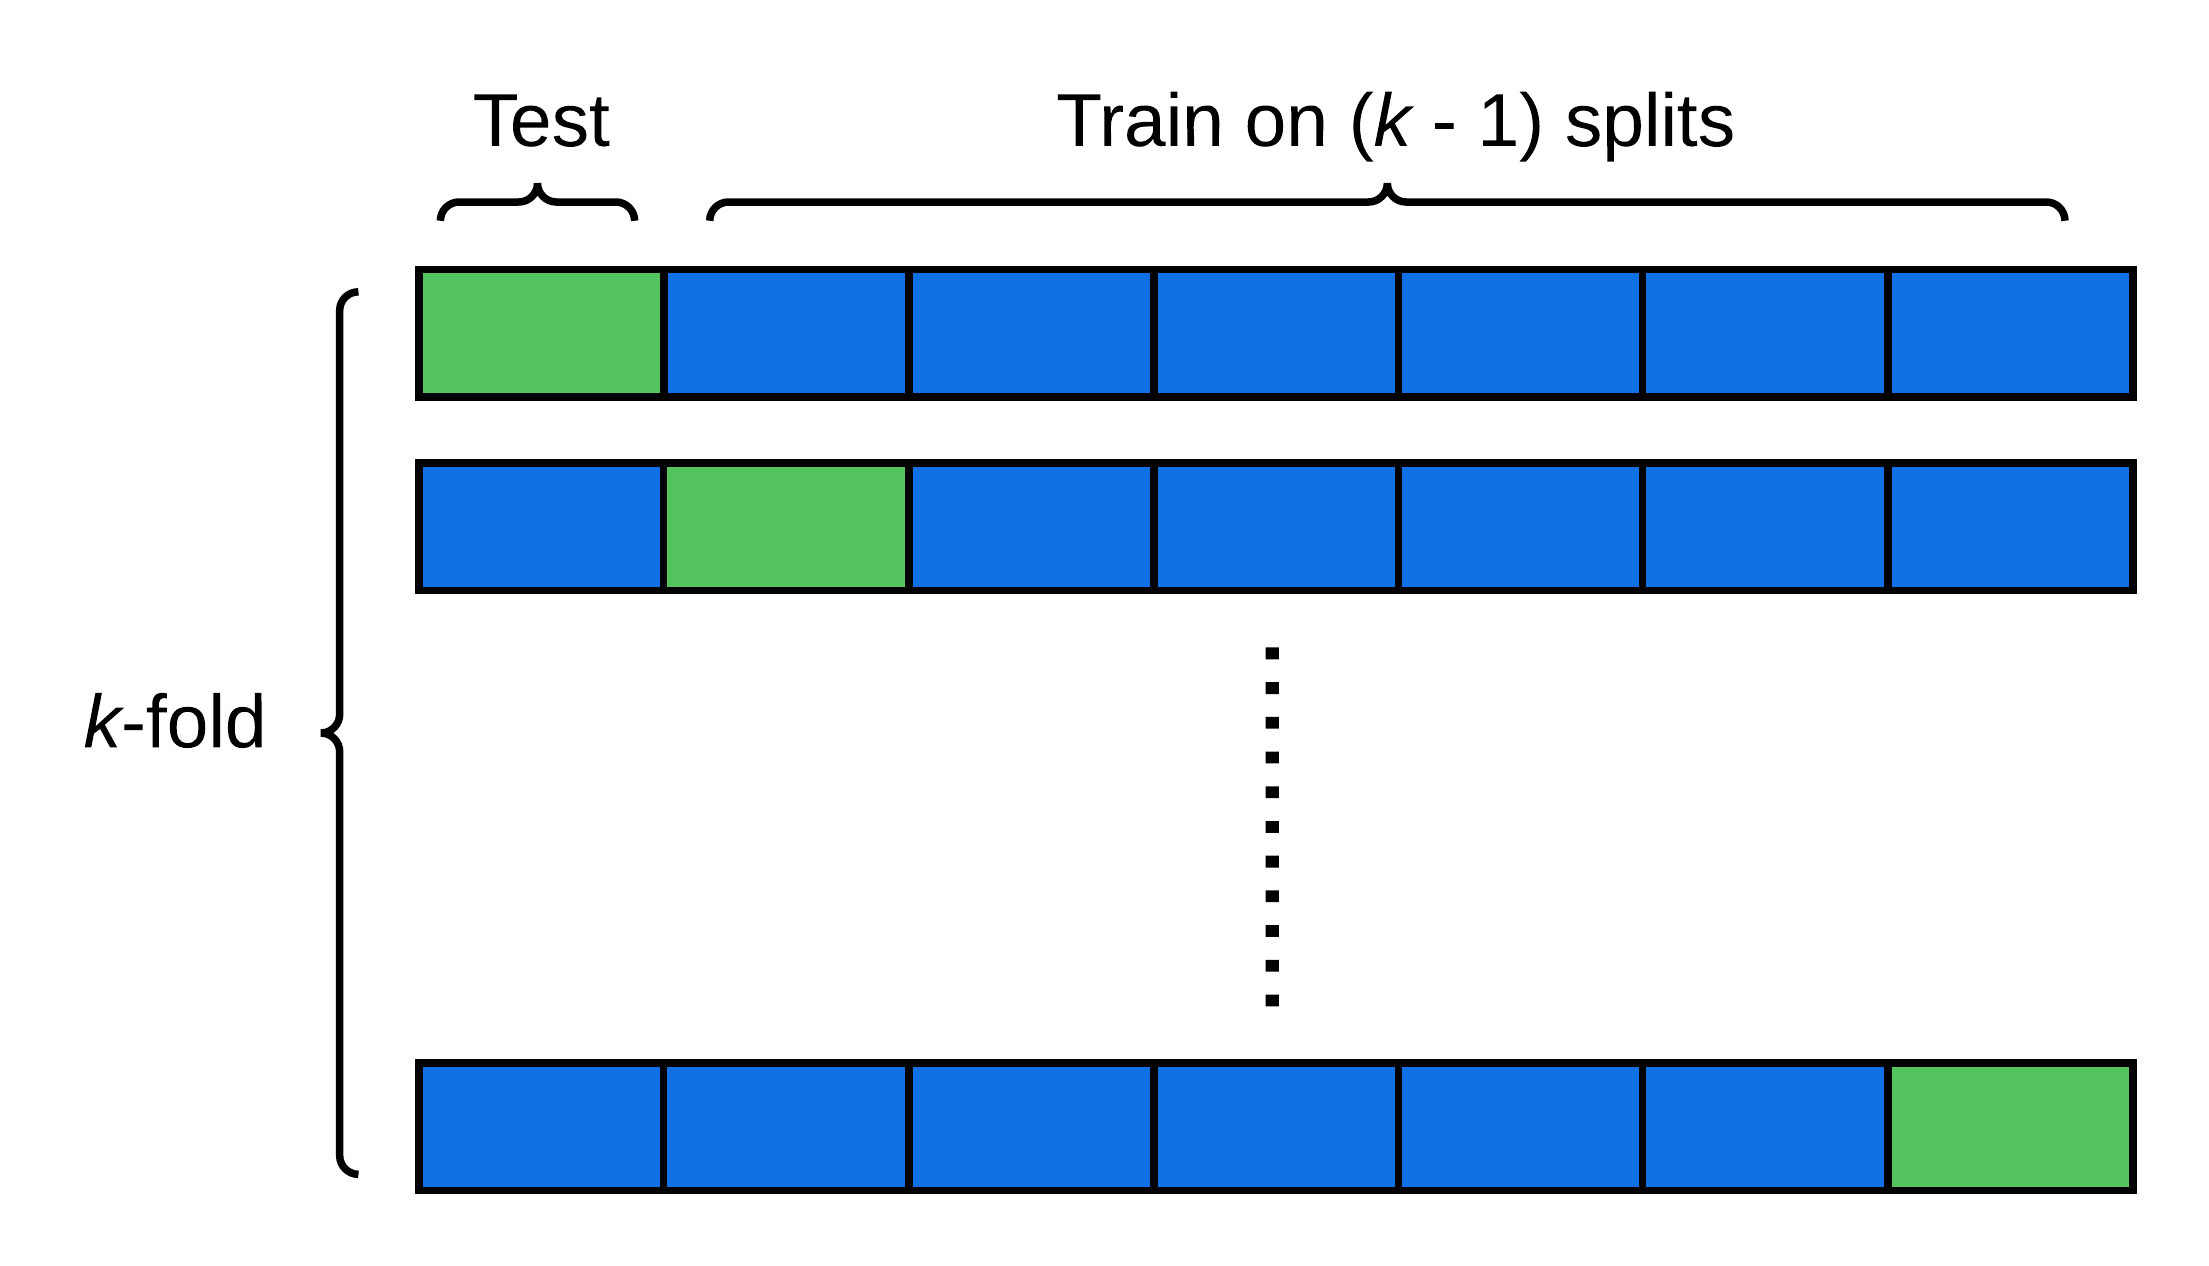
\includegraphics[width=0.6\linewidth]{LOOCV.png}
    \caption{LOOCV algorithm example on \textit{k} folds}
    \label{fig:LOOCV}
\end{figure}

However, LOOCV has some downsides:
\begin{itemize}
  \item \textbf{Computational Cost:} It can be computationally expensive, especially on large datasets, as it requires a significant number of separate model trainings. 
  Training the model repeatedly for each sample can be time-consuming and resource-intensive.
  \item \textbf{Variance:} In some cases, LOOCV may have high variance because it relies on the performance of a single sample as the test set in each iteration. 
  This can lead to variability in the estimated performance.
\end{itemize}  
    
\subsection{Evaluation Metrics}
\label{subsec:evaluation_metrics}

Evaluation metrics in ML are fundamental tools for measuring the effectiveness and accuracy of predictive models.
These metrics provide a clear overview of the model's performance and assist in making informed decisions during the development and optimization process. \\

The \textbf{confusion matrix} is an essential tool used in the evaluation of classification models in ML.
It provides a detailed overview of a model's performance by comparing the model's predictions with the actual class labels of the test data. \\
The confusion matrix consists of four main elements:

\begin{itemize}

\item{\textbf{True Positives (TP)}: The model correctly predicted a positive class. 
For example, if we are trying to identify spam emails, and the model correctly classified an email as spam, it is a True Positive.}
\item{\textbf{True Negatives (TN)}: The model correctly predicted a negative class.}
\item{\textbf{False Positives (FP)}: The model incorrectly predicted a positive class when it was actually negative. This is also referred to as \textit{Type I error}.} 
\item{\textbf{False Negatives (FN)}: The model incorrectly predicted a negative class when it was actually positive. This is also referred to as \textit{Type II error}.}
\end{itemize}

\begin{figure}[H]
  \centering
  \renewcommand{\arraystretch}{2} % Aumenta lo spazio tra le righe del doppio
  \begin{tabular}{|>{\rule[-0.5cm]{0pt}{1.5cm}}c|c|c|}
  \hline
  \backslashbox{Real}{Pred} & Negative &  Positive\\
  \hline
  Negative & TN & FP \\
  \hline
  Positive & FN & TP \\
  \hline
  \end{tabular}
  \caption{Example of confusion matrix}
  \label{tab:conf_matrix}
\end{figure}

The confusion matrix is an important resource for calculating various evaluation metrics such as:


\begin{itemize}
  \item{

  \textbf{Accuracy} is a measure of the overall percentage of correct predictions made by a classification model.

  \begin{equation}
    \textit{Accuracy} = \frac{\text{TP + TN}}{\text{TP + TN + FP + FN}}
    \label{formula:accuracy}
  \end{equation}

  }
  \item{

  \textbf{TSS} or True Skill Statistic is a evaluation metric excellent for imbalanced datasets. 
  TSS, in these cases, performs better than Accuracy, which might appear high despite the poor prediction of TP.

  \begin{equation}
    \textit{TSS} = \frac{\text{TN}}{\text{TN + FP}} + \frac{\text{TP}}{\text{TP + FN}} - 1
    \label{formula:tss}
  \end{equation}

  }
  \item{

  \textbf{Precision} measures the percentage of positive predictions made by the model that are actually correct.

  \begin{equation}
    \textit{Precision} = \frac{\text{TP}}{\text{TP + FP}}
    \label{formula:precision}
  \end{equation}

  }
  \item{

  \textbf{Recall} (also known as Sensitivity)  measures the percentage of actual positive cases that were correctly predicted by the model.

  \begin{equation}
    \textit{Recall} = \frac{\text{TP}}{\text{TP + FN}}
    \label{formula:recall}
  \end{equation}

  }
  \item{

  \textbf{F1-score} is a measure that combines precision and recall into a single value to evaluate the overall performance of the model.


  \begin{equation}
    \textit{F1-score} = \frac{2 \cdot \textit{Recall} \cdot \textit{Precision}}{\textit{Recall} + \textit{Precision}}
    \label{formula:f1}
  \end{equation}
  
  }
\end{itemize} 


The \textbf{Receiver Operating Characteristic} (ROC) curve  is a fundamental tool in ML and statistics for evaluating and visualizing the performance of binary classification models. 
It provides valuable insights into how well a model can distinguish between two classes (binary classification) across different classification thresholds.
For a more comprehensive evaluation of a model's performance across various thresholds, 
it is advisable to utilize a model that can provide probability scores for both classes rather than relying solely on categorical classifications.
Components of the ROC Curve are:

\begin{itemize}
  \item \textbf{True Positive Rate} (TPR) also known as $Sensitivity$ or $Recall$ (\ref{formula:recall}).
  
  \item \textbf{True Negative Rate} (TNR), also known as $Specificity$, is the ratio of true negative instances to the total actual negative instances:
  \begin{equation}
    \textit{TNR} = \frac{\text{TN}}{\text{TN + FP}}
    \label{formula:trueNegativeRate}
  \end{equation}

  \item \textbf{False Positive Rate} (FPR) is the ratio of negative instances misclassified as positive to the total actual negative instances:
  \begin{equation}
    \textit{FPR} = \frac{\text{FP}}{\text{FP + TN}}
    \label{formula:falsePositiveRate}
  \end{equation}

  \item \textbf{Classification Thresholds:} ROC curves are created by varying the classification threshold (the point at which the model decides whether a sample belongs to the positive or negative class) and observing how TPR and FPR change at each threshold.
\end{itemize}
Plotting the ROC Curve consists of:
\begin{enumerate}
  \item Start by sorting the instances by their predicted probabilities or scores.
  \item Begin with a threshold that classifies all instances as positive, resulting in a point at (0, 0) on the ROC curve.
  \item Gradually lower the threshold, moving along the sorted instances, and calculate TPR and FPR at each step.
  \item Plot TPR on the y-axis and FPR on the x-axis, creating the ROC curve.
\end{enumerate}
A random classifier (the same as flipping a coin for every prediction) would produce a diagonal line from (0,0) to (1,1), so a good model should have an ROC curve that is above this line.\\

\textbf{Area Under the ROC Curve} (AUC-ROC):
The AUC-ROC quantifies the overall performance of a binary classification model. It represents the area under the ROC curve.
A perfect model has an AUC-ROC of 1, indicating it can perfectly distinguish between positive and negative cases.
A random or poorly performing model has an AUC-ROC of approximately 0.5, resulting in a diagonal ROC curve.
Typically, the higher the AUC-ROC, the better the model's ability to discriminate between classes.
ROC curves provide a visual depiction of a model's trade-off between \textit{Sensitivity} and \textit{Specificity} (1 - FPR) across different classification thresholds.
In Figure \ref{fig:ROC_AUC}, it is shown an illustration of three distinct curves, each accompanied by its corresponding area value.\\

In binary classification, the class prediction for each instance is often made based on a continuous random variable \textit{X}, which is a $score$ computed for the instance (e.g. the estimated probability in logistic regression). 
Given a threshold parameter \textit{T}, the instance is classified as \textit{positive} if $X > T$, and \textit{negative} otherwise. 
Changing the threshold \textit{x*} along a curve corresponds to shifting the position of the black vertical line in Figure \ref{fig:PNDistribution}. 
The underlying idea is that a perfect classifier achieves a distinct separation between the two classes (0 for negative and 1 for positive), enabling an ideal thresholding operation.
In the case of an imperfect classifier, there exists a tradeoff between FP and FN.
\begin{figure}[H]
  \centering
  \begin{subfigure}{0.8\linewidth}
    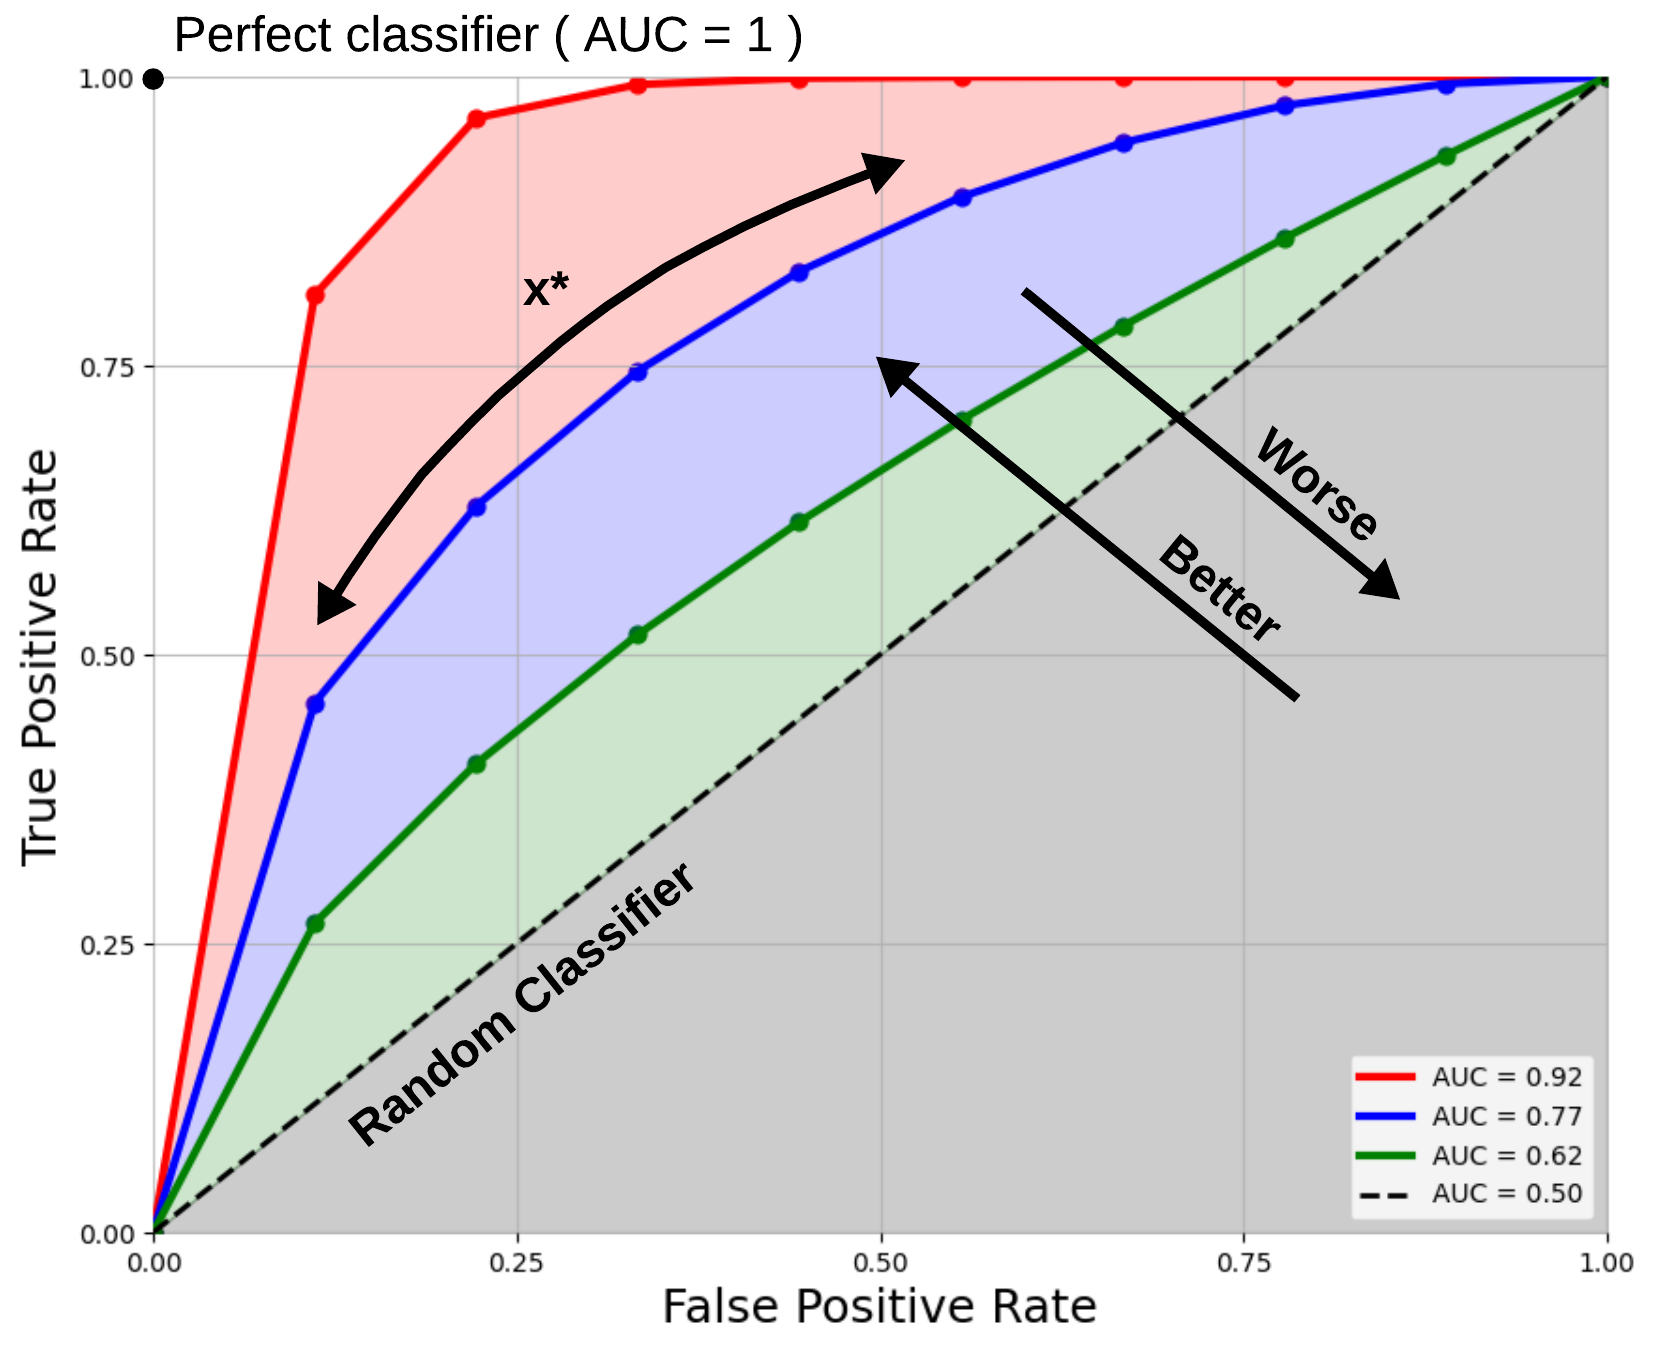
\includegraphics[width=\linewidth]{ROC_AUC.png}
    \caption{}
    \label{fig:ROC_AUC}
  \end{subfigure}
  \begin{subfigure}{0.8\linewidth}
    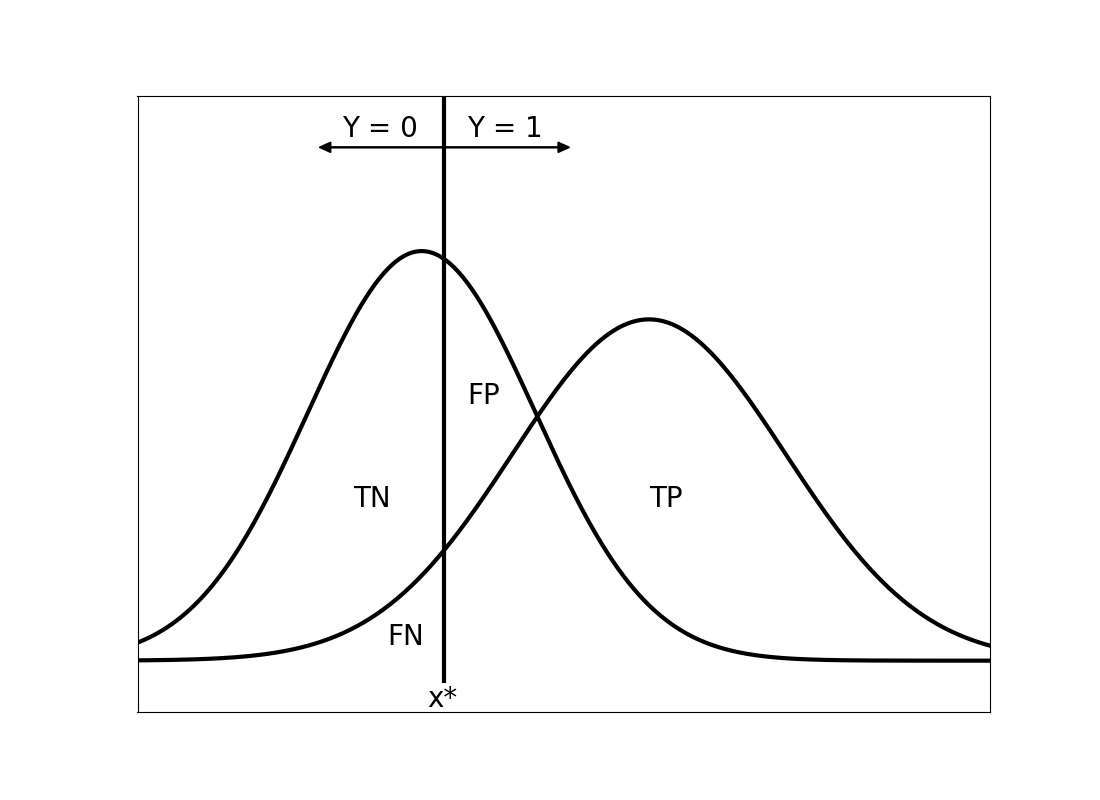
\includegraphics[width=\linewidth]{PN_Distribution_Thresholded.png}
    \caption{}
    \label{fig:PNDistribution}
  \end{subfigure}
  \caption{ROC curves, AUC and thresholds applied on the data distribution}
  \label{fig:ROC}
\end{figure}
\part{Dataset details}
\chapter{Dataset and Marker Set}
\label{chapter:dataset}
A critical phase in our research is the creation of a relevant and high-quality dataset, 
as the quality of the dataset can significantly impact the outcomes of our research efforts.
Here, we detail the methodology used to collect the dataset and its constituents.
Our primary objective is to develop an automated method for detecting the initiation of full-body human movements and identifying the most effective predictive movement features.
Central to this research is capturing motion dynamics accurately.
The participation of these skilled dancers is crucial because their deep knowledge of body mechanics leads to precise and high-quality motion data.
This collaboration yields expressive movements with distinct starting points, aligning with research goals.
Their expertise increases dataset quality, providing a resource that encapsulates human motion intricacies accurately and artistically.

\section{Raw Data Sources}
\label{sec:dataset}
The dataset contains two categories of expressive movements, each associated with a different recording session.
The details of both types of movements are provided below.\\
These segments represents various participants performing simple movement sequences, which are captured from different angles using some cameras.
The videos are synchronized through SMPTE timecode and each video is accompanied by corresponding motion capture data that records the positions of body parts.
The systems used for the recording are different versions of the same software, the \textit{Qualisys Motion Capture system}.


\subsection{WhoLoDance Dataset}
This specific portion of the dataset was collected within the framework of the H2020-ICT-2015 EU Project named $WhoLoDance$.
during the month of March in 2016.
These recording sessions are primarily characterized by their multimodal nature, 
meaning that they involve the use of multiple data recording methods. 
The primary focus during these sessions was on capturing expressive aspects of movement, 
specifically qualities related to movement dynamics. These qualities encompassed various factors, 
including the origin of movement, lightness, fluidity, and more.
The participants in these sessions are professional dancers 
who prepared for their recording sessions by designing a series of exercises in advance. 
The recorded movements primarily revolved around contemporary dance techniques. 
Importantly, these movements were performed without any accompanying music to ensure that 
the dancers' performances were not influenced by external auditory cues.

\subsection{Montpellier - UniGe Dataset}
This specific subset of the dataset was captured during a collaborative project involving the University of Genova and the University of Montpellier in July 2020. 
These recording sessions are divided into two segments: individual actions and dual actions. 
The primary aim of these action categories is to identify the source or initiator of motion in purposeful movements.\\
\underline{Action: Grasping}\\
From the trials that entail individual actions we took some that involves an individual grasping a object. 
In this scenario, participants are positioned in a way that they are facing an object situated at a distance equal to the length 
of their shoulder and at an angle of 20 degrees in the outward direction from the front of their dominant shoulder. 
Participants are instructed to reach for the object with their dominant hand in a natural and spontaneous manner and then place it in front of their non-dominant side.\\
\underline{Action: Throwing}\\
Participants are instructed to perform a two-handed throw, where in one scenario, 
the participant throws the ball and retrieves it themselves, while in the other scenario, two participants throw the ball to each other. 
This was done to introduce greater movement diversity.
It is worth noting that, for the purpose of motion analysis, the receiver and the thrower are considered separately.

\section{Original Marker Set}
\label{sec:orig_markers}
Due to a four-year gap between the recording of the two distinct subsets of the dataset, 
some differences in marker technology have emerged. 
In particular, the WhoLoDance recordings feature a full marker set consisting of 64 reflective markers. 
In contrast, the Montpellier-Unige recordings utilize the newer Qualisys sport marker set, comprising 41 markers. 
Nevertheless, the fundamental principles guiding the marker placement and grouping remain consistent for both datasets. 
The following figures (Figure \ref{fig:64markers}, Figure \ref{fig:41markers}) represent the body mapping of the different markers set. 

\begin{figure}[H]
    \centering
    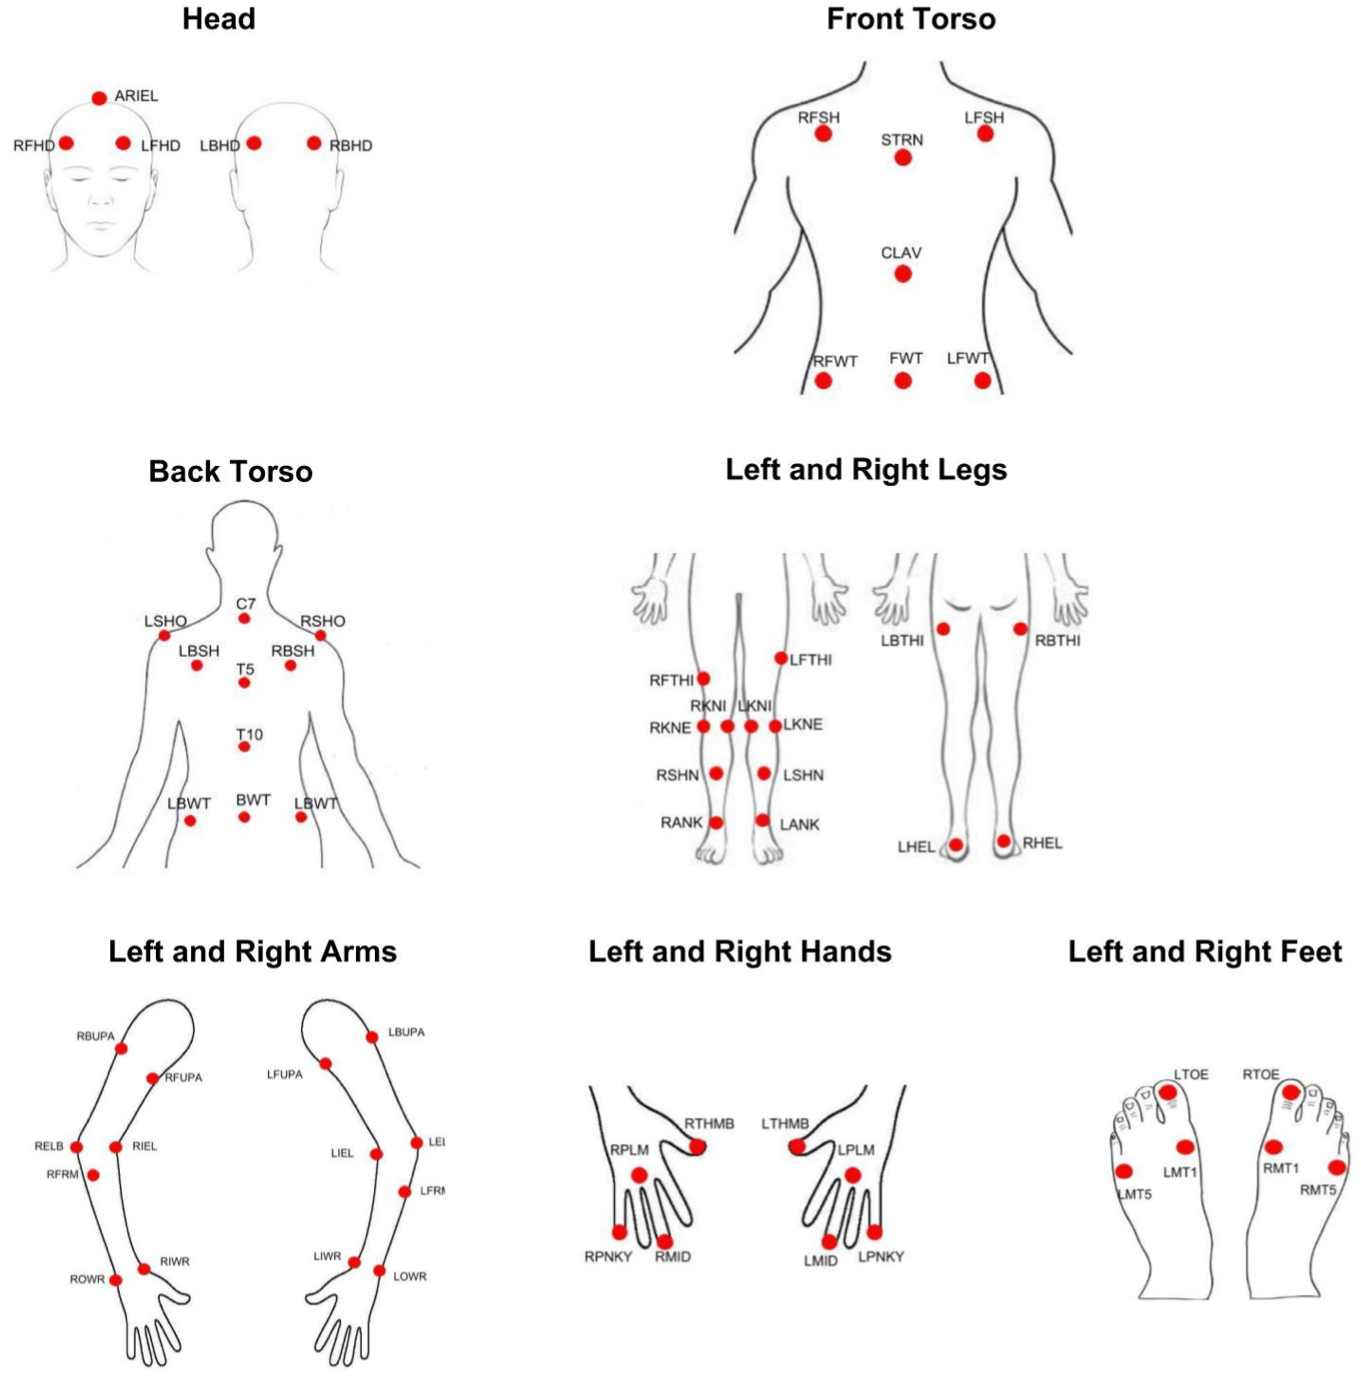
\includegraphics[width=\textwidth]{full_marker_set.png}
    \caption{Markers Set with 64 Labels}
    \label{fig:64markers}
\end{figure}

\begin{figure}[H]
    \centering
    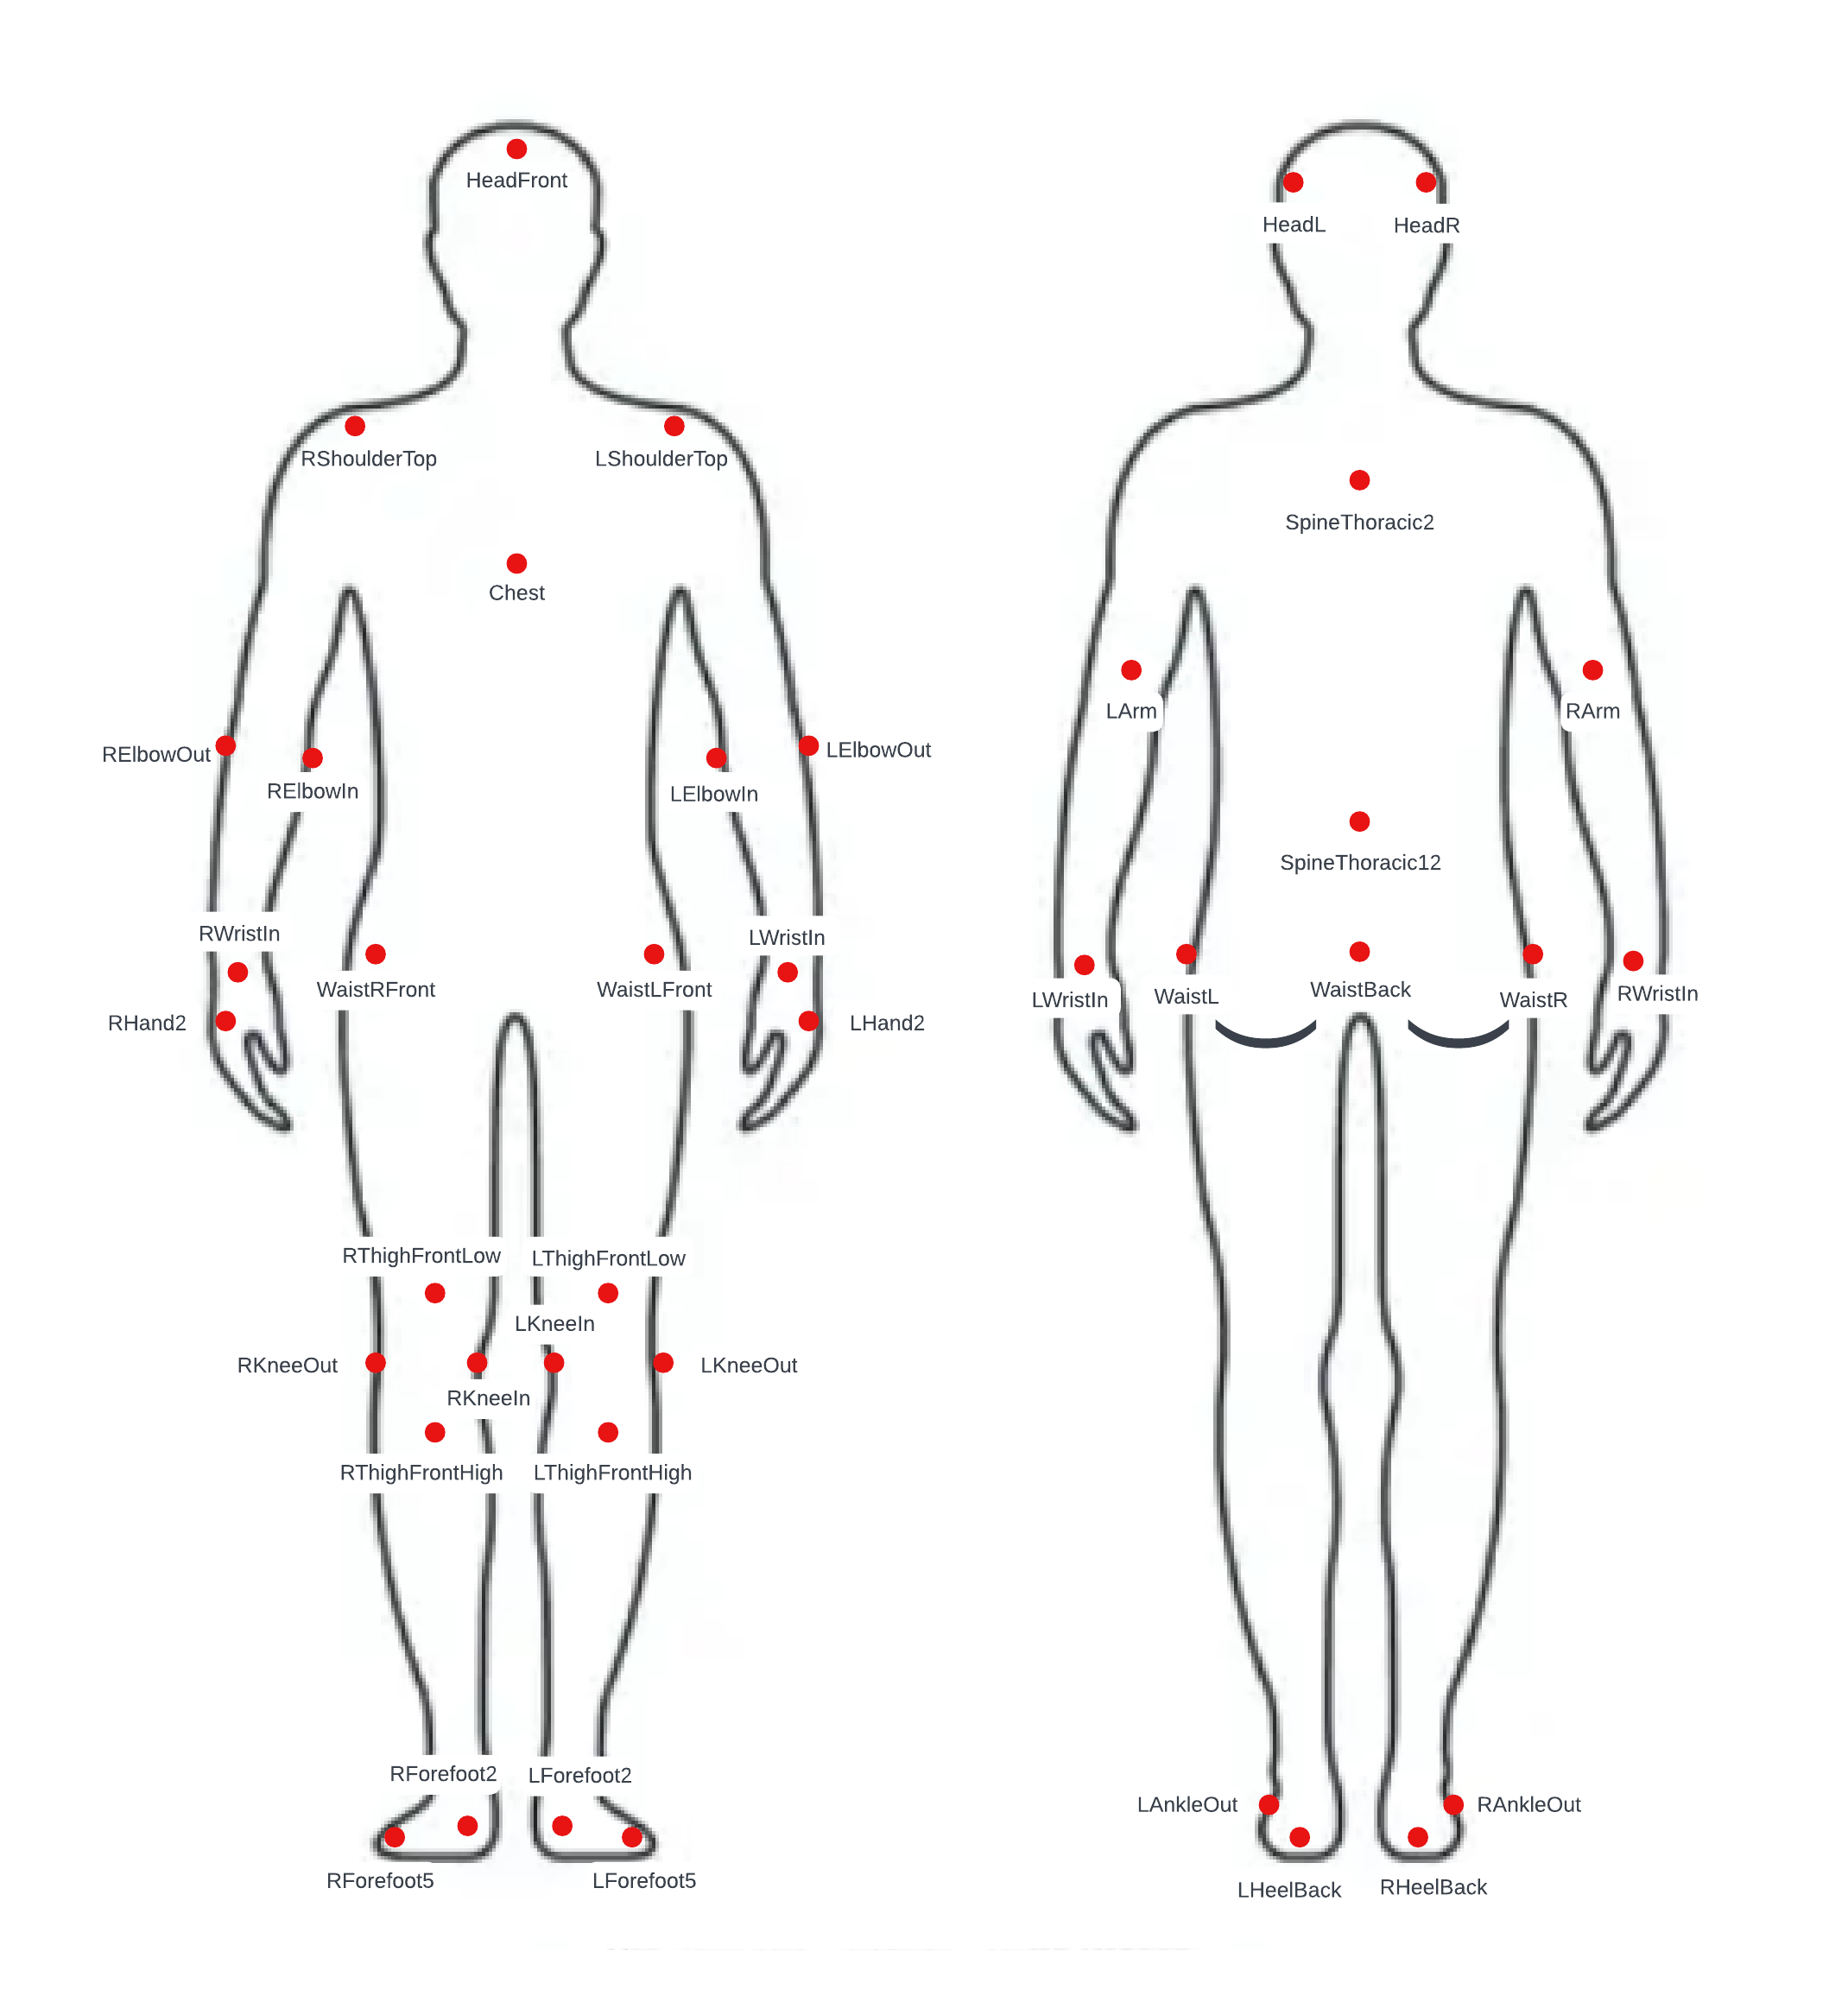
\includegraphics[width=\textwidth]{41Markers.png}
    \caption{Markers Set with 41 Labels}
    \label{fig:41markers}
\end{figure}
\clearpage
\section{Reduced Marker Set}
\label{sec:reduced_markers}
Firstly, we standardized the marker labels following the 64-marker scheme, 
we renamed some of the 41-marker labels to align with the full version (Table \ref{tab:marker_mapping_41}).

The reduced marker set is achieved by reducing the count of markers employed from the full marker set.
This because a simplified skeletal framework can adeptly communicate essential insights about expressive movements.
The reduction process involved computing the \textit{barycenter} of grouped joints, following the specified grouping scheme provided in Table \ref{tab:marker_mapping_64}. 
Initially, the coordinates ($x$, $y$, $z$) for each marker within the cluster were extracted. 
Subsequently, the averages of each cohordinate was calculated.
The joints are considered all equally weighted.

\begin{table}[H]
    \centering
    \begin{tabular}{||c||c||}
    \hline
    \textbf{41 Sport Marker Set Labels} & \textbf{64 Marker Set Labels} \\
    \hline
    RKneeIn, LKneeIn & RKNI, LKNI \\
    HeadFront, HeadL, HeadR & ARIEL, LFHD, RFHD \\
    Chest & STRN \\
    WaistLFront, WaistRFront & LFWT, RFWT \\
    LShoulderTop, RShoulderTop & LSHO, RSHO \\
    SpineThoracic2, SpineThoracic12 & C7, T10 \\
    WaistBack, WaistL, WaistR & BWT, LBWT, RBWT \\
    LKneeOut, RKneeOut & LKNE, RKNE \\
    LHeelBack, RHeelBack & LHEL, RHEL \\
    LAnkleOut, RAnkleOut & LANK, RANK \\
    LForefoot2, LForefoot5, RForefoot2, RForefoot5& LTOE, LMT5, RTOE, RMT5\\
    LHand2, RHand2 & LPLM, RPLM \\
    LWristIn, LWristOut, RWristIn, RWristOut & LIWR, LOWR, RIWR, ROWR \\
    LElbowIn, LElbowOut, RElbowIn, RElbowOut & LIEL, LELB, RIEL, RELB \\
    \hline
    \end{tabular}
    \caption{41 Markers renaming convention}
    \label{tab:marker_mapping_41}
\end{table}

\begin{table}[H]
    \centering
    \begin{tabular}{||c||c||}
        \hline
        \textbf{Reduced Marker Set Labels} & \textbf{Partition of the 64 Marker Set Labels} \\
        \hline
        right\_foot & RHEL, RMT1, RMT5, RTOE \\
        left\_foot & LHEL, LMT1, LMT5, LTOE \\
        right\_ankle & RANK \\
        left\_ankle & LANK \\
        right\_knee & RKNE, RKNI \\
        left\_knee & LKNE, LKNI \\
        right\_hip & RFWT, RBWT \\
        hip\_center & RFWT, LFWT, RBWT, LBWT \\
        left\_hip & LFWT, LBWT \\
        spine & C6, C7, T5, T10, BWT, STRN, CLAV, FWT \\
        right\_hand & RPLM, RTHMB, RINDX, RMID, RPNKY\\
        left\_hand & LPLM, LTHMB, LINDX, LMID, LPNKY \\
        right\_wrist & ROWR, RIWR \\
        left\_wrist & LOWR, LIWR \\
        right\_elbow & RELB, RIEL, RFRM\\
        left\_elbow & LELB, LIEL, LFRM \\
        right\_shoulder & RSHO \\
        shoulder\_center & LSHO, RSHO \\
        left\_shoulder & LSHO \\
        head & RBHD, LBHD, LFHD, RFHD, ARIEL \\
        \hline
    \end{tabular}
    \caption{Mapping of the full marker set to the reduced marker set}
    \label{tab:marker_mapping_64}
\end{table}

\clearpage
\section{Annotations}
\label{sec:annotations}
Starting from the recordings of movements from these sources, we selected about one hundred segments in which we could clearly identify the origin of the movement.\\
Each video fragment was given a label corresponding to the edge between two joints that was deemed to be the origin of the movement.\\
The labelling process was carried out by individually labelling half of the segments. Then we compared our labels and considered for our dataset only those on which we agreed without any a-priori knowledge on the other's opinion.
We proposed those labels to our professors and considered for the dataset only those on which all of us agreed.
The final selection was made merging our labels with the opinion of an expert dancer.\\
This process was used to include only the segments where the labelling was more certain and evident.\\ 

The ending result comprises an amount of 60 fragments, divided between 58 recordings coming from the "WhoLoDance" and 2 from the "Montpellier - Unige" session. 
It spaced over 15 of the 20 joints available, the others are discarted during refinement process.
Unfortunately, the dataset obtained ended up being unbalanced, meaning that there are some labels that are very frequent, some that are infrequent, and some labels that are completely absent.
In Figure \ref{fig:dataset_distribution} we can see the resulting distribution of each edge as the origin of movement.\\

\begin{figure}[H]
    \centering
    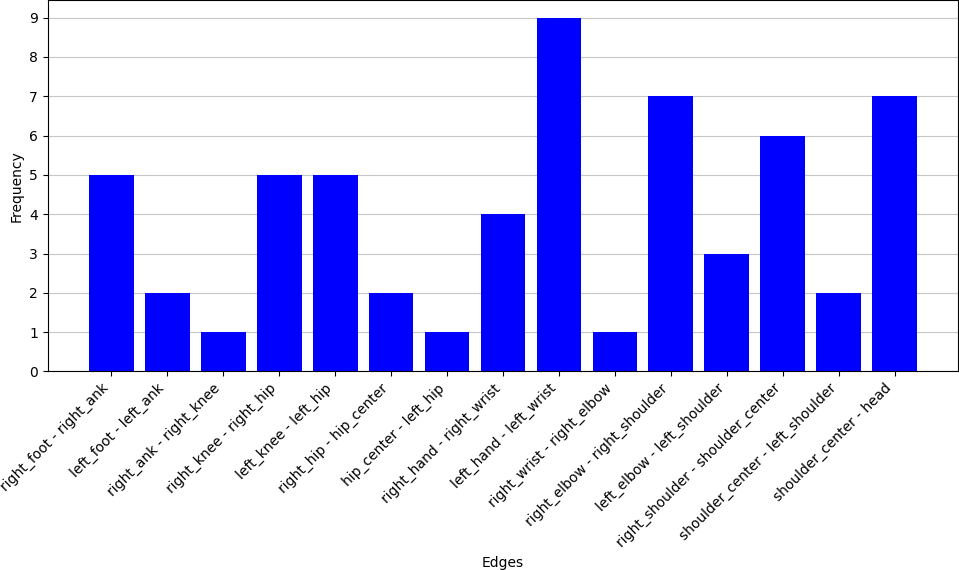
\includegraphics[width=\textwidth]{datasetDistribution.png}
    \caption{Edges frequencies in the Dataset}
    \label{fig:dataset_distribution}
\end{figure}
\part{Cluster visualization}
\chapter{Graph Skeletal Structure}
The Graph Skeletal Structure is obtained considering the \textit{reduced marker set}, obtained after the reduction from the \textit{full marker set} which has been discussed previously. \\
We model the human skeleton as an undirected graph, where the vertices are the joints and the edges represent connections between consecutive physical body joints.\\
Each edge is associated with a specific weight, the value of which depend on a feature extracted from motion capture data. \\
From this \textit{graph skeletal structure}, we define a mathematical game in which the vertices are the players and the edges model the communication channels (through which movement can propagate) between these players. \\
In figure we can see the \textit{graph skeletal structure} without and a table with the joints' labels.
For simplicity, the links are without weights.

\begin{figure}[H]
  \centering
  \begin{subfigure}[b]{0.7\linewidth}
    \centering
    \begin{tikzpicture}
      \node[circle, draw, minimum size=0.8cm] (1) at (1, 0) [] {1};
      \node[circle, draw, minimum size=0.8cm] (2) at (9, 0) [] {2};
      \node[circle, draw, minimum size=0.8cm] (3) at (2.5, 0.9375) [] {3};
      \node[circle, draw, minimum size=0.8cm] (4) at (7.5, 0.9375) [] {4};
      \node[circle, draw, minimum size=0.8cm] (5) at (3, 2.8125) [] {5};
      \node[circle, draw, minimum size=0.8cm] (6) at (7, 2.8125) [] {6};
      \node[circle, draw, minimum size=0.8cm] (7) at (3.5, 5) [] {7};
      \node[circle, draw, minimum size=0.8cm] (8) at (5, 6.25) [] {8};
      \node[circle, draw, minimum size=0.8cm] (9) at (6.5, 5) [] {9};
      \node[circle, draw, minimum size=0.8cm] (10) at (5,8) [] {10};
      \node[circle, draw, minimum size=0.8cm] (11) at (0.7, 7.1875) [] {11};
      \node[circle, draw, minimum size=0.8cm] (12) at (9.3, 7.1875) [] {12};
      \node[circle, draw, minimum size=0.8cm] (13) at (1.7, 7.4) [] {13};
      \node[circle, draw, minimum size=0.8cm] (14) at (8.3, 7.4) [] {14};
      \node[circle, draw, minimum size=0.8cm] (15) at (2.7, 8.6) [] {15};
      \node[circle, draw, minimum size=0.8cm] (16) at (7.3, 8.6) [] {16};
      \node[circle, draw, minimum size=0.8cm] (17) at (3, 10.5) [] {17};
      \node[circle, draw, minimum size=0.8cm] (18) at (5, 10.8375) [] {18};
      \node[circle, draw, minimum size=0.8cm] (19) at (7, 10.5) [] {19};
      \node[circle, draw, minimum size=0.8cm] (20) at (5, 12.5) [] {20};
      
      \foreach \source/\dest/\label/\xshiftval in {20/18//0, 18/17//0, 18/19//0, 17/15//0, 15/13//0, 13/11//0, 19/16//0, 16/14//0, 14/12//0, 18/10//0, 10/8//0, 8/7//0, 7/5//0, 5/3//0, 3/1//0, 8/9//0, 9/6//0, 6/4//0, 4/2//0}
        \path (\source) edge node[xshift=\xshiftval] {\label} (\dest);
    \end{tikzpicture}    
  \end{subfigure}
  \label{fig:graph_skeletal}
  \begin{subfigure}[b]{0.29\linewidth}
    \centering
    \begin{table}[H]
      \centering
      \begin{tabular}{|c|c|}
        \hline
        \textbf{Node} & \textbf{Label} \\
        \hline
        1 & right\_foot \\
        2 & left\_foot \\
        3 & right\_ankle \\
        4 & left\_ankle \\
        5 & right\_knee \\
        6 & left\_knee \\
        7 & right\_hip \\
        8 & hip\_centre \\
        9 & left\_hip \\
        10 & spine \\
        11 & right\_hand \\
        12 & left\_hand \\
        13 & right\_wrist \\
        14 & left\_wrist \\
        15 & right\_elbow \\
        16 & left\_elbow \\
        17 & right\_shoulder \\
        18 & shoulder\_centre \\
        19 & left\_shoulder \\
        20 & head \\
        \hline
      \end{tabular}
    \end{table}
  \end{subfigure}
  \caption{Skeletal structure and nodes names}
  \label{tab:labels_joints}
\end{figure}


\section{Movement features extraction}
\label{sec:features}
The low-level features extracted for our purpose are \textit{speed}, \textit{tangential acceleration}, and \textit{angular momentum}. \\
While speed indicates how quickly an object is moving, acceleration indicates how rapidly its velocity is changing.\\
Angular momentum provides information about the rotation of an object around a fixed point.\\
By incorporating all three quantities as features, a more comprehensive and detailed view of the overall motion is obtained.

\subsection{Speed}
Speed is calculated by finding the change in positions with respect to time through differentiation and then applying a moving average to obtain a more accurate estimate that is less affected by noise.
We calculate this speed as the norm of the velocity vector. \\
The speed of a moving object is a fundamental information in understanding how it moves and how its trajectory might evolve.

\begin{equation}
  \vec{v}(t) = \frac{d\vec{r}}{dt} = \left(\frac{dx}{dt}, \frac{dy}{dt}, \frac{dz}{dt}\right)
\end{equation}

\subsection{Tangential Acceleration}
By calculating the derivative of velocity, we can obtain tangential acceleration.
Tangential acceleration is calculated as the norm of the tangential acceleration vector. \\
Tangential acceleration can be used to express specific emotions, styles, and intentions. \\
For instance, rapid acceleration might be associated with energetic and rhythmic movements, whereas a more gradual acceleration could be linked to fluid and delicate motions.

\begin{equation}
  \vec{a}(t) = \frac{d\vec{v}}{dt} = \left(\frac{d^2x}{dt^2}, \frac{d^2y}{dt^2}, \frac{d^2z}{dt^2}\right)
\end{equation}

\subsection{Angular Momentum}
The angular momentum has been calculated with respect to the center of mass so we proceeded by:
\begin{enumerate}
  \item calculating the relative position with respect to the center of mass as: 
  \begin{figure}[H]
    \centering
    \begin{align}
        \vec{s}_{CM} &= \frac{{\sum_{j=1}^{20} \vec{s}_{j}}}{{20}} &
        \vec{s}_{r} &= \vec{s} - \vec{s}_{CM} \label{eq:rel_pos}
    \end{align}
  \end{figure}
  \item the relative velocity:
  \begin{figure}[H]
    \centering
    \begin{align}
        \vec{v}_{CM} &= \frac{\vec{ds}_{CM}}{dt} &
        \vec{v}_{r} &= \vec{v} - \vec{v}_{\text{CM}} \label{eq:rel_vel}
    \end{align}
  \end{figure}
  \item Then the formula we use to calculate angular momentum relative to the center of mass:
  \begin{figure}[H]
    \centering
    \begin{align}
      \vec{L} = \vec{s}_{r} \times (\vec{v}_{r} * m) \quad with \ m = 1 \ for \ every \ joint \label{eq:ang_mom}
    \end{align}
  \end{figure}
\end{enumerate}

Analyzing angular momentum can reveal specific patterns of rotation or changes in orientation. \\
These patterns can be used to identify distinctive gestures or movements in activities such as gymnastics or choreography.

\section{Similarity measure}
To calculate the weights of the edges connecting the different joints at each instant, we use different formulas depending on the feature we are considering.
\\

\textit{Speed and Acceleration:} in the case of Speed and Acceleration features, for each time instant, we have to introduce a factor of tollerance.\\
$tol_i$ is the tollerance at time instant $i$ and is obtained by computing the mean of all the $features$ at instant $i$ at multipying by a factor 
$10^{-3}$.
\begin{equation}
  tol_i = mean(feature_i) \cdot 10^{-3}
  \label{formula:tol}
\end{equation}
This is done to prevent errors in future calculations such as division by zero.


In the subsequent step, we assign a weight to each edge for every pair of joints $v$ and $\hat{v}$ for each instant $i$:
\begin{itemize}
  \item If the two joints are indeed connected in the skeleton, for example, $left\_hand$ and $left\_wrist$, we use the following formula:
    \begin{equation}
      w^{v\hat{v}}_{i} = \frac{1}{\|feature^{v}_{i}\|-\|feature^{\hat{v}}_{j}\|+tol}
    \end{equation}
  \item If the two joints are not actually connected, for example, $head$ and $right\_foot$, we use the following formula:
    \begin{equation}
      w^{v\hat{v}}_{i} = \frac{1}{5 \cdot (\|feature^{v}_{i}\|-\|feature^{\hat{v}}_{j}\|+tol)}
      \label{formula:tol}
    \end{equation}
\end{itemize}

\textit{Angular Momentum:} in the case of Angular Momentum, we assign a weight to each edge for every pair of joints $v$ and $\hat{v}$ for
each instant $i$, distinguishing between two cases:
\begin{itemize}
  \item If the two joints are indeed connected in the skeleton, we use the following formula:
    \begin{equation}
      w^{v\hat{v}}_{i} = \frac{feature^{v}_{i} \times feature^{\hat{v}}_{i}}{\|feature^{v}_{i}\|-\|feature^{\hat{v}}_{j}\|} + 1
    \end{equation}
  \item If the two joints are not actually connected, we use the following formula:
    \begin{equation}
      w^{v\hat{v}}_{i} = \frac{feature^{v}_{i} \times feature^{\hat{v}}_{i}}{5 \cdot (\|feature^{v}_{i}\|-\|feature^{\hat{v}}_{j}\|+1)}
      \label{formula:tol}
    \end{equation}
\end{itemize}
\chapter{Spectral Clustering}
Clusterization aims to identify groups of nodes that exhibit significant similarity based on the features or data they represent.
This technique is often employed when data is represented as vectors and you want to uncover similarity relationships among these vectors.\\
The Shi-Malik algorithm is a clustering technique based on analyzing the eigenvalues and eigenvectors of the Laplacian matrix of a graph constructed from data.\\
This type of algorithm can be used to partition data into clusters based on their connectivity structure.
Clusterization works to find natural divisions in the graph so that nodes within each cluster are similar to each other based on cosine similarity. \\
The objective is to unveil hidden structures within data so that similar objects are grouped together to aid in data understanding and analysis.
The algorithm has some limitations due to the initialization phase, such as sensitivity to the initial choice of centroids and the requirement to specify the number of clusters beforehand.\\
This is why there will be a subsequent phase of cluster stabilization over time.

\section{Shi-Malik Algorithm}
The operation of the Shi-Malik Algorithm can be summarized in these 8 steps:

\begin{enumerate}
    
  \item \textbf{Calculation of Laplacian Matrix:}
  The Laplacian matrix is the difference between the diagonal matrix of node degrees \(D\) and the similarity matrix \(A\): 

  \begin{equation}
    L = D - A
  \end{equation}
  
  \item \textbf{Calculation of Laplacian's Eigenvectors and Eigenvalues:}
  Eigenvectors and eigenvalues of the Laplacian matrix are calculated using the $\texttt{np.linalg.eig()}$ function. Eigenvectors represent new transformed data features in the eigenvector space, while eigenvalues provide information about the overall variance of data along the corresponding eigenvectors.
  
  \item \textbf{Selection of Eigenvector to use:}
  Eigenvectors are ordered based on their associated eigenvalues. \\
  The eigenvector corresponding to the second-largest eigenvalue is selected (the first eigenvalue corresponds to a constant eigenvector representing scale and is ignored).
  
  \item \textbf{Binarization of Eigenvector:}
  The selected eigenvector is binarized by assigning the value 1 to data points with values greater than 0 in the eigenvector and 0 otherwise. \\
  This process separates the data into two initial groups.
  
  \item \textbf{Cluster Splitting:}
  A recursive cluster splitting algorithm, known as \texttt{split\_a\_cluster}, is applied to further divide clusters into smaller subclusters.
  The option \textit{ncut} is selected as optimization options.
  The sum of weights of data points within the two subclusters is calculated, and the optimal cutting point that minimizes the weight cut is identified.
  The resulting two subclusters are treated separately, and the splitting algorithm is applied to each of them.
  
  \item \textbf{Iterative Cluster Splitting:}
  The splitting algorithm is applied iteratively until a sufficient number of clusters are created to satisfy the desired cluster count $k$.
  At each iteration, points to be split are selected based on the weights of the current clusters.
  The eigenvector associated with each subcluster is computed and used for the next iteration.
  
  \item \textbf{Final Cluster Assignment:}
  At the end of the algorithm, data points are assigned to clusters based on their membership in the obtained subclusters.
  
  \item \textbf{Returning Results:}
  The output of the algorithm is an array of cluster assignments, where each data point is associated with a cluster number.
  
\end{enumerate}

In essence, the algorithm starts by dividing data into two initial clusters, then proceeds with iteratively splitting smaller clusters until the desired number of clusters is achieved.
This method leverages the spectral information of the data graph to obtain a data partition into clusters.


\section{Further Optimization}
The order in which the various clusters are created and chosen is random, and therefore, this randomness can lead to complications in terms of visualization. Hence, there is a need for cluster stabilization over time as a subsequent step. This issue is due to various factors, including:

\begin{enumerate}

    \item \textbf{Eigenvector Sensitivity:}
    The algorithm relies on utilizing the eigenvectors of the Laplacian matrix to define new data features. Eigenvectors can exhibit slight variations in different iterations, especially when eigenvalues are very close to each other. These variations can impact the separation of data into clusters.
    
    \item \textbf{Different Initialization:}
    The initialization of the cluster splitting process can vary across iterations. Since the algorithm begins by dividing data into two clusters, minor differences in the initial choices of points to split can propagate through subsequent iterations and lead to different outcomes.
    
    \item \textbf{Recursive Splitting Process:}
    The recursive cluster splitting algorithm might generate different subclusters in various iterations due to variations in point weights or choices of optimal splitting points. These variations can result in slightly different data partitions.

\end{enumerate}    
\chapter{Temporal stabilization of clusters}

After clustering, we need to reassign colors to the clusters to stabilize them over time. \\
As mentioned before, the order in which clusters are determined at each moment is random, and the selection order of clusters is represented by a color. Therefore, from the initial random color assignment, we aim to transition to a color assignment where two clusters of the same color share as many nodes (joints) as possible between moments.

This is because the random assignment of colors poses visualization issues for the graph. It's possible that from one moment to the next, two clusters with many shared joints might have different colors, resulting in a visualization over time that appears as a continuous switching of colors. This could lead to a loss of continuity in the visual representation.
To stabilize clusters over time, ensuring that pairs of clusters colored from one moment to another share the highest number of common joints, we turn to the MPWM.

We have implemented two algorithms: a BF approach, where we compute the total weights of all possible permutations of color assignments and select the assignment with the maximum total weight, and the Hungarian Algorithm, a combinatorial optimization method that solves the assignment problem in polynomial time.

Since in our case the number of clusters is usually small, there are instances where the BF is more efficient.

\section{Maximum Perfect Weight Matching for bipartite graphs}
The Maximum Perfect Weight Matching is an optimization problem concerning graphs.
The graphs in question are bipartite, meaning the vertices can be divided into two distinct sets in such a way that all edges of the graph connect vertices from different sets, with no edges connecting vertices within the same set.
Additionally, these graphs are undirected, meaning the relationship between two nodes is bidirectional, in other words, the edge connecting node A to node B automatically implies the existence of the edge connecting node B to node A. \\
In the MPWM problem, the vertices represent elements to be paired, and the edges represent possible connections between these elements. 
Each edge is associated with a weight that represents the value or importance of the pairing between the connected vertices.\\
The goal is to find a perfect matching, which is a set of edges in which every node is connected to exactly one other node, with no overlaps or isolated nodes, while maximizing the total weight of the edges in the matching.
The total weight is the sum of the weights of the edges included in the matching.
The weights of the edges are collected in a matrix called a \textit{utility matrix}.\\
The utility matrix will be a square matrix because the number of nodes in the two distinct sets is the same.
The rows could represent the nodes in the first set, while the columns could represent the nodes in the second set, or vice versa.
The element (\textit{i}, \textit{j}) of the matrix represents the weight of the edge connecting vertex \textit{i} to vertex \textit{j}. 


\subsection{Temporal stabilization}
In our case, instead of having nodes connected by edges, we will have a slightly different situation.
Instead of the previously introduced nodes, we will have clusters, which are sets of nodes representing the joints of the skeleton, connected to each other by edges.\\  
Consider the clusters at time \textit{t} and the clusters at time \textit{t+1} as two distinct sets, so there will be no edges connecting clusters that belong to the same set.
Each cluster in one set must be connected by an edge to exactly one cluster in the other set, with the goal of maximizing the total weight of the edges.
The weight of an edge is equal to the number of nodes that the two clusters it is connecting have in common.\\
As previously mentioned, at this stage of the pipeline, we already have information about the joints belonging to various clusters and the colors of these clusters. However, we want to reassign colors to stabilize the visualization over time.
The previous clustering groups the joints into clusters and assigns them random colors, while in this phase of the pipeline, we optimize the color assignment.\\
We will start by analyzing the colors of the clusters at the initial frame and choose the best color assignment for the next frame.
Then will repeat this process iteratively until the last frame.


\subsection{A real application}
Let's consider a real-world scenario to understand how MPWM works in terms of visualization.
Suppose we have 20 nodes representing joints at time \textit{t} and 3 clusters labeled with different colors, as shown in Figure \ref{fig:clust_t}.
At time \textit{t+1}, there are the same 20 nodes as before but with 3 clusters labeled differently (see Figure \ref{fig:clust_tplus1}). \\
Certainly, this clustering-based assignment cannot be regarded as the optimal assignment, as we still need to assess the \textit{3!} possible color assignments. \\
We know the colors of the clusters at time \textit{t}, and we want to assign colors to the clusters at time \textit{t+1}. \\
In Figure \ref{fig:clust_ass}, you can visually see all the possible color assignments, while in Table \ref{tab:table_clust}, all the values of common nodes for each color and the total weight of the matching are gathered.


\begin{figure}[H]
  \centering
  \begin{tikzpicture}
    \node[circle, draw, minimum size=0.7cm] (1) at (1,-9) [fill=green!50] {1};
    \node[circle, draw, minimum size=0.7cm] (2) at (9, -9) [fill=green!50] {2};
    \node[circle, draw, minimum size=0.7cm] (3) at (2.5,-8.5) [fill=green!50] {3};
    \node[circle, draw, minimum size=0.7cm] (4) at (7.5, -8.5) [fill=green!50] {4};
    \node[circle, draw, minimum size=0.7cm] (5) at (3,-6.5) [fill=green!50] {5};
    \node[circle, draw, minimum size=0.7cm] (6) at (7,-6.5) [fill=green!50] {6};
    \node[circle, draw, minimum size=0.7cm] (7) at (3.5,-4.5) [fill=green!50] {7};
    \node[circle, draw, minimum size=0.7cm] (8) at (5, -3.5) [fill=green!50] {8};
    \node[circle, draw, minimum size=0.7cm] (9) at (6.5,-4.5) [fill=green!50] {9};
    \node[circle, draw, minimum size=0.7cm] (10) at (5,-1.5) [fill=green!50] {10};
    \node[circle, draw, minimum size=0.7cm] (11) at (1,-4) [fill=red!50] {11};
    \node[circle, draw, minimum size=0.7cm] (12) at (9,-4) [fill=blue!50] {12};
    \node[circle, draw, minimum size=0.7cm] (13) at (2, -3.5) [fill=red!50] {13};
    \node[circle, draw, minimum size=0.7cm] (14) at (8, -3.5) [fill=blue!50] {14};
    \node[circle, draw, minimum size=0.7cm] (15) at (2.5,-1) [fill=red!50] {15};
    \node[circle, draw, minimum size=0.7cm] (16) at (7.5,-1) [fill=blue!50] {16};
    \node[circle, draw, minimum size=0.7cm] (17) at (3,1) [fill=red!50] {17};
    \node[circle, draw, minimum size=0.7cm] (18) at (5,1.5) [fill=blue!50] {18};
    \node[circle, draw, minimum size=0.7cm] (19) at (7,1) [fill=blue!50] {19};
    \node[circle, draw, minimum size=0.7cm] (20) at (5,3) [fill=blue!50] {20};
    \foreach \source/\dest/\label/\xshiftval in {20/18//0, 18/17//0, 18/19//0, 17/15//0, 15/13/Cluster 2/-45, 13/11//0, 19/16//0, 16/14/Cluster 3/45, 14/12//0, 18/10//0, 10/8//0, 8/7//0, 7/5//0, 5/3/Cluster 1/-45, 3/1//0, 8/9//0, 9/6//0, 6/4//0, 4/2//0}
      \path (\source) edge node[xshift=\xshiftval] {\label} (\dest);
  \end{tikzpicture}
  \caption{Optimal color assignment to clusters at time \textit{t}}
  \label{fig:clust_t}
\end{figure}


\begin{figure}[H]
    \centering
    \begin{tikzpicture}
      \node[circle, draw, minimum size=0.3cm] (1) at (3.5,-1.25) [fill=green!50] {};
      \node[circle, draw, minimum size=0.3cm] (2) at (6.5, -1.25) [fill=red!50] {};
      \node[circle, draw, minimum size=0.3cm] (3) at (4,-1) [fill=green!50] {};
      \node[circle, draw, minimum size=0.3cm] (4) at (6, -1) [fill=red!50] {};
      \node[circle, draw, minimum size=0.3cm] (5) at (4.25,-0.5) [fill=green!50] {};
      \node[circle, draw, minimum size=0.3cm] (6) at (5.75,-0.5) [fill=red!50] {};
      \node[circle, draw, minimum size=0.3cm] (7) at (4.5,0) [fill=green!50] {};
      \node[circle, draw, minimum size=0.3cm] (8) at (5, 0.5) [fill=green!50] {};
      \node[circle, draw, minimum size=0.3cm] (9) at (5.5,0) [fill=red!50] {};
      \node[circle, draw, minimum size=0.3cm] (10) at (5,1.25) [fill=green!50] {};
      \node[circle, draw, minimum size=0.3cm] (11) at (3.2, 0.25) [fill=green!50] {};
      \node[circle, draw, minimum size=0.3cm] (12) at (6.75,0.25) [fill=blue!50] {};
      \node[circle, draw, minimum size=0.3cm] (13) at (3.5, 0.75) [fill=green!50] {};
      \node[circle, draw, minimum size=0.3cm] (14) at (6.5, 0.75) [fill=blue!50] {};
      \node[circle, draw, minimum size=0.3cm] (15) at (3.75,1.5) [fill=green!50] {};
      \node[circle, draw, minimum size=0.3cm] (16) at (6.25,1.5) [fill=blue!50] {};
      \node[circle, draw, minimum size=0.3cm] (17) at (4.25,2) [fill=green!50] {};
      \node[circle, draw, minimum size=0.3cm] (18) at (5,2.25) [fill=green!50] {};
      \node[circle, draw, minimum size=0.3cm] (19) at (5.75,2) [fill=blue!50] {};
      \node[circle, draw, minimum size=0.3cm] (20) at (5,3) [fill=green!50] {};  
      \foreach \source/\dest/\label/\xshiftval in {20/18//0, 18/17//0, 18/19//0, 17/15//0, 15/13//-45, 13/11//0, 19/16//0, 16/14/Cluster 6/45, 14/12//0, 18/10//0, 10/8//0, 8/7//0, 7/5//0, 5/3/Cluster 4/-45, 3/1//0, 8/9//0, 9/6//0, 6/4/Cluster 5/45, 4/2//0}
        \path (\source) edge node[xshift=\xshiftval] {\label} (\dest);
    \end{tikzpicture}
      \caption{Color assignment to clusters at time \textit{t+1} obtained from clustering}
      \label{fig:clust_tplus1}
\end{figure}

\begin{figure}[H]
  \centering
  \begin{subfigure}{0.3\textwidth}
    \centering
    \begin{tikzpicture}[every node/.style={circle, draw, minimum size=0.1cm}]
      \node (1) at (3.5,-1.25) [fill=green!50] {};
      \node (2) at (6.5, -1.25) [fill=red!50] {};
      \node (3) at (4,-1) [fill=green!50] {};
      \node (4) at (6, -1) [fill=red!50] {};
      \node (5) at (4.25,-0.5) [fill=green!50] {};
      \node (6) at (5.75,-0.5) [fill=red!50] {};
      \node (7) at (4.5,0) [fill=green!50] {};
      \node (8) at (5, 0.5) [fill=green!50] {};
      \node (9) at (5.5,0) [fill=red!50] {};
      \node (10) at (5,1.25) [fill=green!50] {};
      \node (11) at (3.2, 0.25) [fill=green!50] {};
      \node (12) at (6.75,0.25) [fill=blue!50] {};
      \node (13) at (3.5, 0.75) [fill=green!50] {};
      \node (14) at (6.5, 0.75) [fill=blue!50] {};
      \node (15) at (3.75,1.5) [fill=green!50] {};
      \node (16) at (6.25,1.5) [fill=blue!50] {};
      \node (17) at (4.25,2) [fill=green!50] {};
      \node (18) at (5,2.25) [fill=green!50] {};
      \node (19) at (5.75,2) [fill=blue!50] {};
      \node (20) at (5,3) [fill=green!50] {};  
      \foreach \source/\dest in {20/18, 18/17, 18/19, 17/15, 15/13, 13/11, 19/16, 16/14, 14/12, 18/10, 10/8, 8/7, 7/5, 5/3, 3/1, 8/9, 9/6, 6/4, 4/2}
        \path (\source) edge (\dest);
    \end{tikzpicture}
      \caption{}
  \end{subfigure}
  \begin{subfigure}{0.3\textwidth}
    \centering
    \begin{tikzpicture}[every node/.style={circle, draw, minimum size=0.1cm}]
      \node (1) at (3.5,-1.25) [fill=green!50] {};
      \node (2) at (6.5, -1.25) [fill=blue!50] {};
      \node (3) at (4,-1) [fill=green!50] {};
      \node (4) at (6, -1) [fill=blue!50] {};
      \node (5) at (4.25,-0.5) [fill=green!50] {};
      \node (6) at (5.75,-0.5) [fill=blue!50] {};
      \node (7) at (4.5,0) [fill=green!50] {};
      \node (8) at (5, 0.5) [fill=green!50] {};
      \node (9) at (5.5,0) [fill=blue!50] {};
      \node (10) at (5,1.25) [fill=green!50] {};
      \node (11) at (3.2, 0.25) [fill=green!50] {};
      \node (12) at (6.75,0.25) [fill=red!50] {};
      \node (13) at (3.5, 0.75) [fill=green!50] {};
      \node (14) at (6.5, 0.75) [fill=red!50] {};
      \node (15) at (3.75,1.5) [fill=green!50] {};
      \node (16) at (6.25,1.5) [fill=red!50] {};
      \node (17) at (4.25,2) [fill=green!50] {};
      \node (18) at (5,2.25) [fill=green!50] {};
      \node (19) at (5.75,2) [fill=red!50] {};
      \node (20) at (5,3) [fill=green!50] {};  
      \foreach \source/\dest in {20/18, 18/17, 18/19, 17/15, 15/13, 13/11, 19/16, 16/14, 14/12, 18/10, 10/8, 8/7, 7/5, 5/3, 3/1, 8/9, 9/6, 6/4, 4/2}
        \path (\source) edge (\dest);
    \end{tikzpicture}
      \caption{}
  \end{subfigure}
  \begin{subfigure}{0.3\textwidth}
    \centering
    \begin{tikzpicture}[every node/.style={circle, draw, minimum size=0.1cm}]
      \node (1) at (3.5,-1.25) [fill=blue!50] {};
      \node (2) at (6.5, -1.25) [fill=red!50] {};
      \node (3) at (4,-1) [fill=blue!50] {};
      \node (4) at (6, -1) [fill=red!50] {};
      \node (5) at (4.25,-0.5) [fill=blue!50] {};
      \node (6) at (5.75,-0.5) [fill=red!50] {};
      \node (7) at (4.5,0) [fill=blue!50] {};
      \node (8) at (5, 0.5) [fill=blue!50] {};
      \node (9) at (5.5,0) [fill=red!50] {};
      \node (10) at (5,1.25) [fill=blue!50] {};
      \node (11) at (3.2, 0.25) [fill=blue!50] {};
      \node (12) at (6.75,0.25) [fill=green!50] {};
      \node (13) at (3.5, 0.75) [fill=blue!50] {};
      \node (14) at (6.5, 0.75) [fill=green!50] {};
      \node (15) at (3.75,1.5) [fill=blue!50] {};
      \node (16) at (6.25,1.5) [fill=green!50] {};
      \node (17) at (4.25,2) [fill=blue!50] {};
      \node (18) at (5,2.25) [fill=blue!50] {};
      \node (19) at (5.75,2) [fill=green!50] {};
      \node (20) at (5,3) [fill=blue!50] {};  
      \foreach \source/\dest in {20/18, 18/17, 18/19, 17/15, 15/13, 13/11, 19/16, 16/14, 14/12, 18/10, 10/8, 8/7, 7/5, 5/3, 3/1, 8/9, 9/6, 6/4, 4/2}
        \path (\source) edge (\dest);
    \end{tikzpicture}
      \caption{}
  \end{subfigure}
  
  \vspace{1cm} % Spazio vuoto tra le righe
  
  \begin{subfigure}{0.3\textwidth}
    \centering
    \begin{tikzpicture}[every node/.style={circle, draw, minimum size=0.1cm}]
      \node (1) at (3.5,-1.25) [fill=blue!50] {};
      \node (2) at (6.5, -1.25) [fill=green!50] {};
      \node (3) at (4,-1) [fill=blue!50] {};
      \node (4) at (6, -1) [fill=green!50] {};
      \node (5) at (4.25,-0.5) [fill=blue!50] {};
      \node (6) at (5.75,-0.5) [fill=green!50] {};
      \node (7) at (4.5,0) [fill=blue!50] {};
      \node (8) at (5, 0.5) [fill=blue!50] {};
      \node (9) at (5.5,0) [fill=green!50] {};
      \node (10) at (5,1.25) [fill=blue!50] {};
      \node (11) at (3.2, 0.25) [fill=blue!50] {};
      \node (12) at (6.75,0.25) [fill=red!50] {};
      \node (13) at (3.5, 0.75) [fill=blue!50] {};
      \node (14) at (6.5, 0.75) [fill=red!50] {};
      \node (15) at (3.75,1.5) [fill=blue!50] {};
      \node (16) at (6.25,1.5) [fill=red!50] {};
      \node (17) at (4.25,2) [fill=blue!50] {};
      \node (18) at (5,2.25) [fill=blue!50] {};
      \node (19) at (5.75,2) [fill=red!50] {};
      \node (20) at (5,3) [fill=blue!50] {};  
      \foreach \source/\dest in {20/18, 18/17, 18/19, 17/15, 15/13, 13/11, 19/16, 16/14, 14/12, 18/10, 10/8, 8/7, 7/5, 5/3, 3/1, 8/9, 9/6, 6/4, 4/2}
        \path (\source) edge (\dest);
    \end{tikzpicture}
      \caption{}
  \end{subfigure}
  \begin{subfigure}{0.3\textwidth}
    \centering
    \begin{tikzpicture}[every node/.style={circle, draw, minimum size=0.1cm}]
      \node (1) at (3.5,-1.25) [fill=red!50] {};
      \node (2) at (6.5, -1.25) [fill=green!50] {};
      \node (3) at (4,-1) [fill=red!50] {};
      \node (4) at (6, -1) [fill=green!50] {};
      \node (5) at (4.25,-0.5) [fill=red!50] {};
      \node (6) at (5.75,-0.5) [fill=green!50] {};
      \node (7) at (4.5,0) [fill=red!50] {};
      \node (8) at (5, 0.5) [fill=red!50] {};
      \node (9) at (5.5,0) [fill=green!50] {};
      \node (10) at (5,1.25) [fill=red!50] {};
      \node (11) at (3.2, 0.25) [fill=red!50] {};
      \node (12) at (6.75,0.25) [fill=blue!50] {};
      \node (13) at (3.5, 0.75) [fill=red!50] {};
      \node (14) at (6.5, 0.75) [fill=blue!50] {};
      \node (15) at (3.75,1.5) [fill=red!50] {};
      \node (16) at (6.25,1.5) [fill=blue!50] {};
      \node (17) at (4.25,2) [fill=red!50] {};
      \node (18) at (5,2.25) [fill=red!50] {};
      \node (19) at (5.75,2) [fill=blue!50] {};
      \node (20) at (5,3) [fill=red!50] {};  
      \foreach \source/\dest in {20/18, 18/17, 18/19, 17/15, 15/13, 13/11, 19/16, 16/14, 14/12, 18/10, 10/8, 8/7, 7/5, 5/3, 3/1, 8/9, 9/6, 6/4, 4/2}
        \path (\source) edge (\dest);
    \end{tikzpicture}
      \caption{}
  \end{subfigure}
  \begin{subfigure}{0.3\textwidth}
    \centering
    \begin{tikzpicture}[every node/.style={circle, draw, minimum size=0.1cm}]
      \node (1) at (3.5,-1.25) [fill=red!50] {};
      \node (2) at (6.5, -1.25) [fill=blue!50] {};
      \node (3) at (4,-1) [fill=red!50] {};
      \node (4) at (6, -1) [fill=blue!50] {};
      \node (5) at (4.25,-0.5) [fill=red!50] {};
      \node (6) at (5.75,-0.5) [fill=blue!50] {};
      \node (7) at (4.5,0) [fill=red!50] {};
      \node (8) at (5, 0.5) [fill=red!50] {};
      \node (9) at (5.5,0) [fill=blue!50] {};
      \node (10) at (5,1.25) [fill=red!50] {};
      \node (11) at (3.2, 0.25) [fill=red!50] {};
      \node (12) at (6.75,0.25) [fill=green!50] {};
      \node (13) at (3.5, 0.75) [fill=red!50] {};
      \node (14) at (6.5, 0.75) [fill=green!50] {};
      \node (15) at (3.75,1.5) [fill=red!50] {};
      \node (16) at (6.25,1.5) [fill=green!50] {};
      \node (17) at (4.25,2) [fill=red!50] {};
      \node (18) at (5,2.25) [fill=red!50] {};
      \node (19) at (5.75,2) [fill=green!50] {};
      \node (20) at (5,3) [fill=red!50] {};  
      \foreach \source/\dest in {20/18, 18/17, 18/19, 17/15, 15/13, 13/11, 19/16, 16/14, 14/12, 18/10, 10/8, 8/7, 7/5, 5/3, 3/1, 8/9, 9/6, 6/4, 4/2}
        \path (\source) edge (\dest);
    \end{tikzpicture}
      \caption{}
  \end{subfigure}

  \vspace{0.5cm} % Spazio vuoto tra le righe
  
  \caption{Possible color assignments at time \textit{t+1}}
  \label{fig:clust_ass}
\end{figure}



\begin{table}[H]
  \centering
  \begin{tabular}{|c|c|c|c|c|}
    \hline
   \textbf{Assignment} & \textbf{Red match} & \textbf{Blue match} & \textbf{Green match} & \textbf{Utility Value} \\
    \hline
    (a) & 0 & 4 & 6 & 10 \\
    \hline
    (b) & 0 & 0 & 6 & 6 \\
    \hline
    (c) & 0 & 2 & 0 & 2 \\
    \hline
    (d) & 0 & 2 & 4 & 6 \\
    \hline
    (e) & 4 & 4 & 4 & 12 \\
    \hline
    (f) & 4 & 0 & 0 & 4 \\
    \hline
  \end{tabular}
  
  \vspace{0.5cm} % Spazio vuoto tra le righe
  
  \caption{Matching weights for the 6 assignments}
  \label{tab:table_clust}
\end{table}
 
From Table \ref{tab:table_clust}, it can be observed that assignment (e) has the highest utility value.
Additionally, even visually, it can be noticed that it is the most consistent assignment compared to the one at time \textit{t}.
\\

From the perspective of Bipartite Matching, we can consider the clusters from Figure \ref{fig:clust_t} in the first partition, while in the second partition, we can consider the clusters from Figure \ref{fig:clust_tplus1}.
As mentioned earlier, the weight of an edge is equivalent to the number of nodes that the two clusters being connected by that edge have in common. \\
The following figure shows the matching with the utility value for every possible assignment and the colored ones for the optimal one.

\begin{figure}[H]
  \centering
  \begin{tikzpicture}
    \node[circle, draw, minimum size=1cm, fill=green!50] (1) at (2,-6.5) {Cluster 1};
    \node[circle, draw, minimum size=1cm, fill=red!50] (2) at (2, -10) {Cluster 2};
    \node[circle, draw, minimum size=1cm, fill=blue!50] (3) at (2,-13.5) {Cluster 3};
    \node[circle, draw, minimum size=1cm, fill=red!50] (4) at (8, -6.5) {Cluster 4};
    \node[circle, draw, minimum size=1cm, fill=green!50] (5) at (8,-10) {Cluster 5};
    \node[circle, draw, minimum size=1cm, fill=blue!50] (6) at (8,-13.5) {Cluster 6};
    
    \foreach \source/\dest/\label/\position/\yshiftval/\xshiftval/\edgecolor in {
      1/4/6/above/0/0/black, 1/5/4/above/25/-40/green, 1/6/0/above/60/-70/black,
      2/4/4/below/-15/-60/red, 2/5/0/below/0/-40/black, 2/6/0/below/30/-60/black,
      3/4/2/below/-60/-70/black, 3/5/0/below/-25/-40/black, 3/6/4/below/0/0/blue}
      \path (\source) edge[\edgecolor, ->,>=stealth, line width=0.5pt] node[\position, yshift=\yshiftval, xshift=\xshiftval, black] {\label} (\dest);
  \end{tikzpicture}
  \caption{Bipartite Matching from instant \textit{t} to instant \textit{t+1}}
  \label{fig:clust_match}
\end{figure}



\section{Brute Force Algorithm}
The BF can be a possible approach to solve the MPWM problem for bipartite graphs.
However, it's important to note that the BF has exponential time complexity, specifically, its time complexity grows exponentially with the number of vertices in the graph.
This is because the BF examines all possible combinations of perfect matchings within the bipartite graph to find the one with the maximum weight.\\
If the graph has \textit{n} vertices in both the first and second partitions, there are \textit{n}!\ possible matchings.
Each matching requires \textit{O}(\textit{n}) time to be computed because you need to check that it is a perfect matching and calculate its total weight.
Therefore, the overall complexity of the algorithm is on the order of \textit{O}(\textit{n}!$\cdot$\textit{n}). \\
Since the complexity grows rapidly as \textit{n} increases, it quickly becomes impractical for large-sized graphs. However, for our case, this is not a problem.

A MPWM problem using an utility matrix can be transformed into a minimum-weight matching problem.
This can be achieved by introducing an auxiliary matrix, referred to as the \textit{cost matrix}.
The cost matrix is essentially a duplicate of the utility matrix, but with all its elements negated.

\subsection{Brute Force Algorithm summarized}
The operation of the BF for minimum-weight matching problems can be summerized in these 3 steps:

\begin{enumerate}
    \item {Compute the cost matrix for the considered bipartite graph with \textit{n} vertices in each partition.}
    \item {Compute the total cost of all the \textit{n}!\ permutations.}
    \item {Choose the assignment with the lowest total cost.}
\end{enumerate}


\subsection{Brute Force Algorithm application}

Let's take for example the following cost matrix and try to apply the BF for minimum-weight matching problems:

\begin{table}[H]
    \centering
    \begin{tabular}{|>{\centering\arraybackslash}m{0.6cm}|>{\centering\arraybackslash}m{0.6cm}|>{\centering\arraybackslash}m{0.6cm}|}
      \hline
      108 & 125 & 150 \\
      \hline
      150 & 135 & 175 \\
      \hline
      122 & 148 & 250 \\
      \hline
    \end{tabular}
    \end{table}

Now we compute the total cost of all the \textit{n}!\ permutations: 
  

  \begin{table}[H]
    \begin{minipage}[b]{0.3\textwidth}
        \centering
        \begin{tabular}{|>{\centering\arraybackslash}m{0.6cm}|>{\centering\arraybackslash}m{0.6cm}|>{\centering\arraybackslash}m{0.6cm}|}
            \hline
            \cellcolor{yellow!25} 108 & 125 & 150 \\
            \hline
            150 & \cellcolor{yellow!25} 135 & 175 \\
            \hline
            \cellcolor{yellow!25} 122 & 148 & 250 \\
            \hline
        \end{tabular}
        \caption*{(a)}
        \label{tab:perm1}
    \end{minipage}
    \hfill
    \begin{minipage}[b]{0.3\textwidth}
        \centering
        \begin{tabular}{|>{\centering\arraybackslash}m{0.6cm}|>{\centering\arraybackslash}m{0.6cm}|>{\centering\arraybackslash}m{0.6cm}|}
            \hline
            108 & \cellcolor{yellow!25} 125 & 150 \\
            \hline
            \cellcolor{yellow!25} 150 & 135 & 175 \\
            \hline
            122 & 148 & \cellcolor{yellow!25} 250 \\
            \hline
        \end{tabular}
        \caption*{(b)}
        \label{tab:perm2}
    \end{minipage}
    \hfill
    \begin{minipage}[b]{0.3\textwidth}
        \centering
        \begin{tabular}{|>{\centering\arraybackslash}m{0.6cm}|>{\centering\arraybackslash}m{0.6cm}|>{\centering\arraybackslash}m{0.6cm}|}
            \hline
            108 & 125 & \cellcolor{yellow!25} 150 \\
            \hline
            150 & \cellcolor{yellow!25} 135 & 175 \\
            \hline
            \cellcolor{yellow!25} 122 & 148 & 250 \\
            \hline
        \end{tabular}
        \caption*{(c)}
        \label{tab:perm3}
    \end{minipage}
\end{table}

\begin{table}[H]
    \begin{minipage}[b]{0.3\textwidth}
        \centering
        \begin{tabular}{|>{\centering\arraybackslash}m{0.6cm}|>{\centering\arraybackslash}m{0.6cm}|>{\centering\arraybackslash}m{0.6cm}|}
            \hline
            \cellcolor{yellow!25} 108 & 125 & 150 \\
            \hline
            150 & \cellcolor{yellow!25} 135 & 175 \\
            \hline
            \cellcolor{yellow!25} 122 & 148 & 250 \\
            \hline
        \end{tabular}
        \caption*{(d)}
        \label{tab:perm4}
    \end{minipage}
    \hfill
    \begin{minipage}[b]{0.3\textwidth}
        \centering
        \begin{tabular}{|>{\centering\arraybackslash}m{0.6cm}|>{\centering\arraybackslash}m{0.6cm}|>{\centering\arraybackslash}m{0.6cm}|}
            \hline
            108 & \cellcolor{yellow!25} 125 & 150 \\
            \hline
            \cellcolor{yellow!25} 150 & 135 & 175 \\
            \hline
            122 & 148 & \cellcolor{yellow!25} 250 \\
            \hline
        \end{tabular}
        \caption*{(e)}
        \label{tab:perm5}
    \end{minipage}
    \hfill
    \begin{minipage}[b]{0.3\textwidth}
        \centering
        \begin{tabular}{|>{\centering\arraybackslash}m{0.6cm}|>{\centering\arraybackslash}m{0.6cm}|>{\centering\arraybackslash}m{0.6cm}|}
            \hline
            108 & 125 & \cellcolor{yellow!25} 150 \\
            \hline
            \cellcolor{yellow!25} 150 & 135 & 175 \\
            \hline
            122 & \cellcolor{yellow!25} 148 & 250 \\
            \hline
        \end{tabular}
        \caption{(f)}
        \label{tab:perm6}
    \end{minipage}
\caption{BF assignements}
\label{tab:tab_ass}
\end{table}
 

\begin{table}[H]
  \centering
  \begin{tabular}{|c|c|c|c|c|}
    \hline
   \textbf{Assignment} & \textbf{Total weight} \\
    \hline
    (a) & 493 \\
    \hline
    (b) & 422 \\
    \hline
    (c) & 448 \\
    \hline
    (d) & 407 \\
    \hline
    (e) & 525 \\
    \hline
    (f) & 431 \\
    \hline
  \end{tabular}
  
  \vspace{0.5cm} % Spazio vuoto tra le righe
  
  \caption{Total weights for the 6 assignments}
  \label{tab:table_costs}
\end{table}

We find that the minimum total cost is given by the assignment (d) in Table \ref{tab:tab_ass}.  


\part{Automatic classification}
\chapter{Clustering}

\section{Auxiliary Graph}
From the clustered graph a weighted auxiliary graph is defined for each frame, denoted as $G^{aux}$ := ($V$, $E^{aux}$, $w^{aux}$). \\
The vertices of this auxiliary graph are the same as in the original graph $G$, but the edge set is comprised of a subset of edges that only connect vertices belonging to different clusters.
The weight of every edge is calculated by applying Euclidean norm (Formula \ref{formula:normalization}) between pairs of vectors.
Edges that do not represent direct physical connections are ignored.
One of these edges in the auxiliary graph will be the edge associated with the origin of motion.
\\

Considering, for example, a graph $G$ with 3 clusters (see Figure \ref{fig:graph_g}), we can visualize which edges will be involved in the auxiliary graph (Figure \ref{fig:aux_graph}).
\begin{figure}[H]
  \begin{subfigure}{0.45\textwidth}
    \centering
    \begin{tikzpicture}
      \node[circle, draw, minimum size=0.1cm] (1) at (3.5,-1.25) [fill=green!50] {};
      \node[circle, draw, minimum size=0.1cm] (2) at (6.5, -1.25) [fill=red!50] {};
      \node[circle, draw, minimum size=0.1cm] (3) at (4,-1) [fill=green!50] {};
      \node[circle, draw, minimum size=0.1cm] (4) at (6, -1) [fill=red!50] {};
      \node[circle, draw, minimum size=0.1cm] (5) at (4.25,-0.5) [fill=green!50] {};
      \node[circle, draw, minimum size=0.1cm] (6) at (5.75,-0.5) [fill=red!50] {};
      \node[circle, draw, minimum size=0.1cm] (7) at (4.5,0) [fill=green!50] {};
      \node[circle, draw, minimum size=0.1cm] (8) at (5, 0.5) [fill=green!50] {};
      \node[circle, draw, minimum size=0.1cm] (9) at (5.5,0) [fill=red!50] {};
      \node[circle, draw, minimum size=0.1cm] (10) at (5,1.25) [fill=green!50] {};
      \node[circle, draw, minimum size=0.1cm] (11) at (3.2, 0.25) [fill=green!50] {};
      \node[circle, draw, minimum size=0.1cm] (12) at (6.75,0.25) [fill=blue!50] {};
      \node[circle, draw, minimum size=0.1cm] (13) at (3.5, 0.75) [fill=green!50] {};
      \node[circle, draw, minimum size=0.1cm] (14) at (6.5, 0.75) [fill=blue!50] {};
      \node[circle, draw, minimum size=0.1cm] (15) at (3.75,1.5) [fill=green!50] {};
      \node[circle, draw, minimum size=0.1cm] (16) at (6.25,1.5) [fill=blue!50] {};
      \node[circle, draw, minimum size=0.1cm] (17) at (4.25,2) [fill=green!50] {};
      \node[circle, draw, minimum size=0.1cm] (18) at (5,2.25) [fill=green!50] {};
      \node[circle, draw, minimum size=0.1cm] (19) at (5.75,2) [fill=blue!50] {};
      \node[circle, draw, minimum size=0.1cm] (20) at (5,3) [fill=green!50] {};  
      \foreach \source/\dest/\label/\xshiftval in {20/18//0, 18/17//0, 18/19//0, 17/15//0, 15/13//0, 13/11//0, 19/16//0, 16/14//0, 14/12//0, 18/10//0, 10/8//0, 8/7//0, 7/5//0, 5/3//0, 3/1//0, 8/9//0, 9/6//0, 6/4//0, 4/2//0}
        \path (\source) edge node[xshift=\xshiftval] {\label} (\dest);
    \end{tikzpicture}
    \caption{Graph $G$}
    \label{fig:graph_g}
  \end{subfigure}
  \hspace{0.01\linewidth}
  \begin{subfigure}{0.45\linewidth}
    \centering
    \begin{tikzpicture}
      \node[circle, draw, minimum size=0.1cm] (1) at (3.5,-1.25) [fill=green!50] {};
      \node[circle, draw, minimum size=0.1cm] (2) at (6.5, -1.25) [fill=red!50] {};
      \node[circle, draw, minimum size=0.1cm] (3) at (4,-1) [fill=green!50] {};
      \node[circle, draw, minimum size=0.1cm] (4) at (6, -1) [fill=red!50] {};
      \node[circle, draw, minimum size=0.1cm] (5) at (4.25,-0.5) [fill=green!50] {};
      \node[circle, draw, minimum size=0.1cm] (6) at (5.75,-0.5) [fill=red!50] {};
      \node[circle, draw, minimum size=0.1cm] (7) at (4.5,0) [fill=green!50] {};
      \node[circle, draw, minimum size=0.1cm] (8) at (5, 0.5) [fill=green!50] {};
      \node[circle, draw, minimum size=0.1cm] (9) at (5.5,0) [fill=red!50] {};
      \node[circle, draw, minimum size=0.1cm] (10) at (5,1.25) [fill=green!50] {};
      \node[circle, draw, minimum size=0.1cm] (11) at (3.2, 0.25) [fill=green!50] {};
      \node[circle, draw, minimum size=0.1cm] (12) at (6.75,0.25) [fill=blue!50] {};
      \node[circle, draw, minimum size=0.1cm] (13) at (3.5, 0.75) [fill=green!50] {};
      \node[circle, draw, minimum size=0.1cm] (14) at (6.5, 0.75) [fill=blue!50] {};
      \node[circle, draw, minimum size=0.1cm] (15) at (3.75,1.5) [fill=green!50] {};
      \node[circle, draw, minimum size=0.1cm] (16) at (6.25,1.5) [fill=blue!50] {};
      \node[circle, draw, minimum size=0.1cm] (17) at (4.25,2) [fill=green!50] {};
      \node[circle, draw, minimum size=0.1cm] (18) at (5,2.25) [fill=green!50] {};
      \node[circle, draw, minimum size=0.1cm] (19) at (5.75,2) [fill=blue!50] {};
      \node[circle, draw, minimum size=0.1cm] (20) at (5,3) [fill=green!50] {};  
      \foreach \source/\dest/\label/\xshiftval in {18/19//0, 8/9//0}
        \path (\source) edge node[xshift=\xshiftval] {\label} (\dest);
    \end{tikzpicture}
    \caption{Auxiliary graph $G^{aux}$}
    \label{fig:aux_graph}
  \end{subfigure}
\end{figure}


\section{Weighted Degree Centrality}
To identify the edge involved in the OoM, we use the WDC, as explained in Section \ref{subsec:weighted_degree}.
For each frame, we keep track of the two nodes with the highest WDC.
At the end of this process, among the selected nodes, we will choose the two nodes that have been chosen as the highest most frequently.
At this stage, we will examine in the $G^{aux}$ to which edges belonging to $E^{aux}$ these two winning nodes are connected, and these two edges will be considered as the predicted OoM.

\section{Results}
The OoM was classified using three distinct features: speed, acceleration and angular momentum, as described in Section \ref{sec:features}.
For each feature, we calculated the accuracy of the method in predicting the correct edge compared to the true label.\\
In Table \ref{tab:clust_results} we can see the results.


\begin{table}[H]
  \centering
  \begin{tabular}{|>{\centering\arraybackslash}p{1.2cm}|>{\centering\arraybackslash}p{4.3cm}|>{\centering\arraybackslash}p{4.3cm}|>{\centering\arraybackslash}p{4.3cm}|}
  \hline
  & \textbf{Speed} & \textbf{Acceleration} & \textbf{Angular Momentum} \\
  \hline
  \textbf{WDG} & 28.3\%  & 26.7\%  & 36.6\%  \\
  \hline
  \end{tabular}
  \caption{Classification accuracy with WDC on the overall dataset}
  \label{tab:clust_results}
\end{table}

Even though these results are not impressive, they are still better than a random approach, where two random nodes are selected, and by examining which edges in the auxiliary graph they are connected to, they are compared to the ground truth. \\
Such an approach, in fact, achieves an accuracy of 19\%.
In the Figure \ref{fig:wdc_results} is the distribution of the results for each edge of the dataset:
\begin{figure}
  \centering
  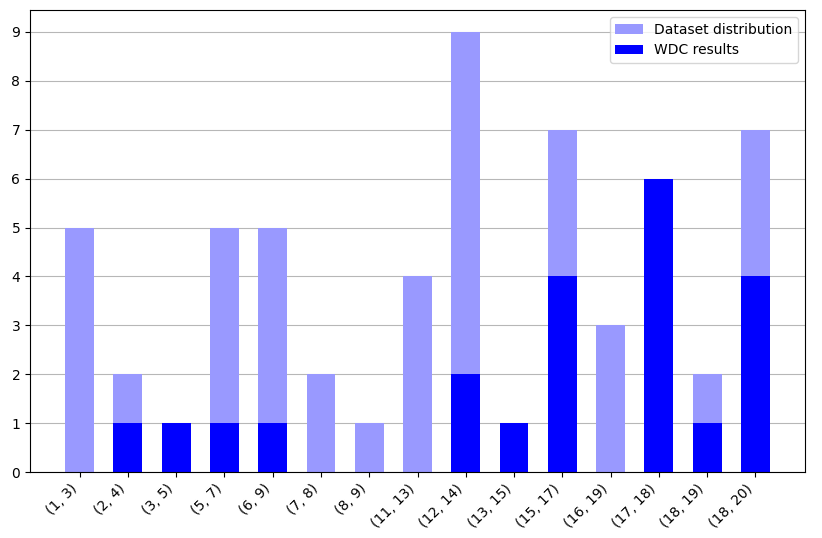
\includegraphics[width=0.85\textwidth]{graphics/wdc_results.png}
  \caption{Joints and frequency of the dataset and the correctly classified WDC algorithm}
  \label{fig:wdc_results}
\end{figure}
\chapter{Machine Learning}

\section{Frames Sampling}
To address the variable length of segments within the dataset, in instances where we aim to attain a lower number of frames than the actual length of the segments, 
we have utilized the "uniform spacing" sampling technique to address the variability in segment lengths within the dataset.
This method entails selecting frames from a list or sequence at regular, even intervals. 
It proves to be highly advantageous when the goal is to ensure an equal distribution of frames throughout the sequence.

\begin{figure}[H]
    \centering
    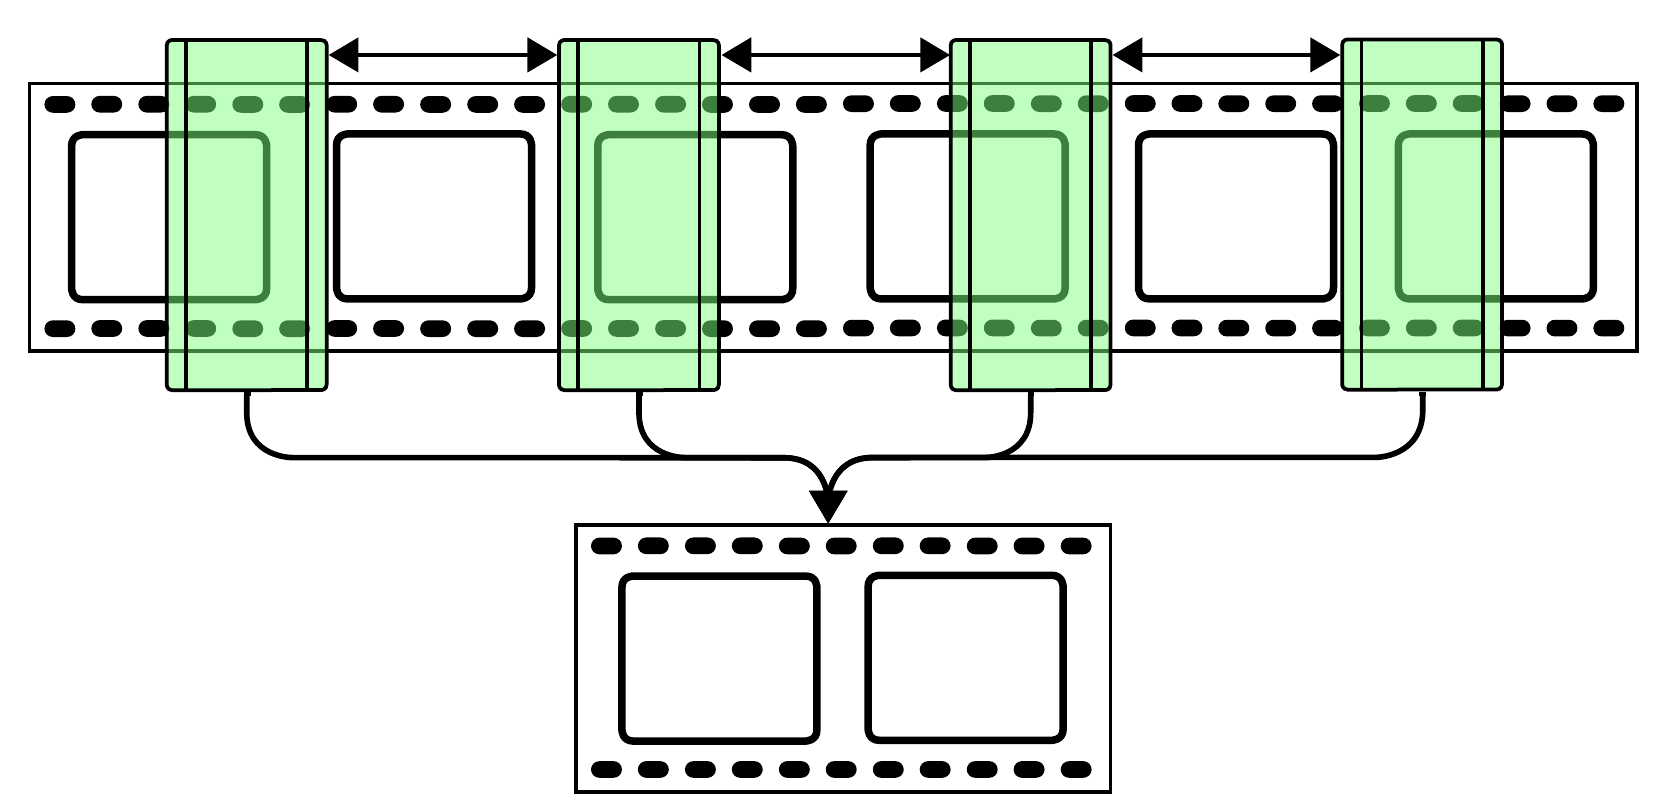
\includegraphics[width=0.8\textwidth]{graphics/subSampling.png}
    \caption{Uniform Sampling visualized}
    \label{fig:unif_sampling}
\end{figure}

Conversely, when dealing with segments that are shorter than the standard number of frames, a different technique is implemented.
In such cases, for each frame, a variable and uniform number of interpolation frames are inserted to reach the desired frame count. 
This approach compensates for the shorter segment length by adding interpolated frames, maintaining the consistency required for further analysis or processing.
\begin{figure}[H]
    \centering
    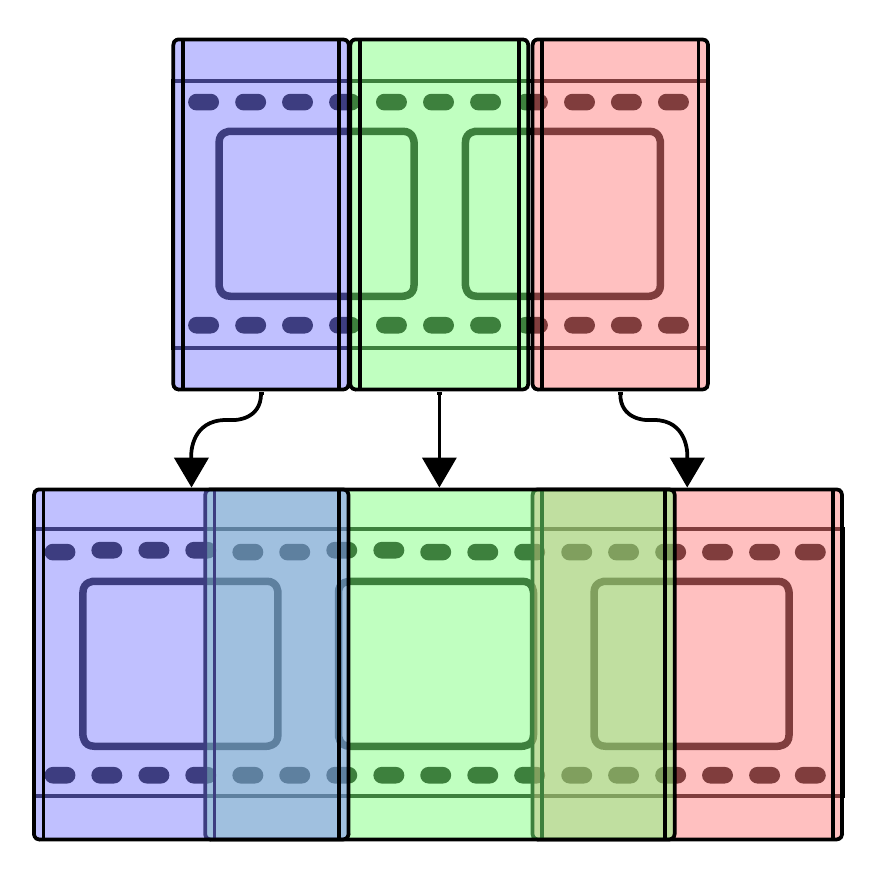
\includegraphics[width=0.4\textwidth]{graphics/interpolationSampling.png}
    \caption{Frames interpolation visualized}
    \label{fig:interp_sampling}
\end{figure}

\section{Dataset Normalization}
As previously mentioned, our dataset consists of 60 samples, each containing the spatial positions of all 20 skeletal joints at each time step.
From the equally sampled timeseries we calculate the $x$, $y$, and $z$ coordinates of the skeleton's barycenter for each time step. \\
We define the barycenter as the point where all the mass of an object or a system of objects is concentrated. \\
In this context, each joint is considered to have unit mass, meaning that all joints contribute equally to the barycenter. \\
If we represent $n$ as the number of 20 joints, the coordinates of the barycenter are obtained by taking the average of the coordinates of these 20 joints, as we can see in the formula:


\begin{equation}
    Barycenter (x, y, z) = \left(\frac{1}{n} \sum_{i=1}^{n} x_i, \frac{1}{n} \sum_{i=1}^{n} y_i, \frac{1}{n} \sum_{i=1}^{n} z_i\right)
    \label{formula:baricentro}
\end{equation}
    
where $x_i$, $y_i$, and $z_i$ represent the $x$, $y$, and $z$ coordinates of the $i$-th joint, respectively.

Subsequently, we calculate the distance between each joint and the barycenter, at each time step, using the Euclidean distance in Formula \ref{formula:distance}. \\
These distances from the barycenter will be normalized for each joint, in order to obtain normalized time series between 0 and 1.

\begin{equation}
    x_{norm} = \frac{{x - min(x)}}{{max(x) - min(x)}}
    \label{formula:normalization}
\end{equation}
    
The choice to calculate the distances between joints and the barycenter for each sample plays a crucial role in ensuring the robustness of our ML approach to variations in scale.
In scenarios where dancers or subjects may have different heights or body proportions, relying solely on absolute joint coordinates could introduce bias into the model.
However, by computing these distances and further normalizing them within the range of 0 to 1, we effectively eliminate the influence of scale variations.

This normalization process not only standardizes the data but also allows the ML model to focus on the relative spatial distribution of joints rather than their absolute positions.
Consequently, our model becomes better equipped to recognize patterns and movements across individuals of varying statures, making it more versatile and applicable in real-world scenarios. \\

\section{Features extraction}
Feature extraction in ML is an essential process that involves transforming raw data into a more suitable format for analysis and model building.
It helps identify and capture the most relevant information within the data while simplifying excessive complexity that could make model training challenging.
This process not only contributes to improving model accuracy but also reduces the risk of overfitting and enhances the ability to generalize knowledge gained to new data. \\
From the preprocessed data, we want to extract the necessary features for ML.
Here we will see al the steps involved in order to achieve the desired features. \\


Finally, to choose the features to extract, we referred to \cite{oneto:2020} and \cite{sama:2010}.
In Table \ref{tab:ml_features} we can see all the features and their relative function.

\begin{table}[H]
    \centering
    \begin{tabular}{|c|c|}
        \hline
        \textbf{Function} & \textbf{Description} \\
        \hline
        mean & Mean Value \\
        var & Variance \\
        mad & Median Absolute Value \\
        max & Largest Value in Array \\
        min & Smallest Value in Array \\
        sma & Signal Magnitude Area \\
        energy & Average Sum of Squares \\
        iqr & Interquantile Range \\
        entropy & Signal Entropy \\
        correlation & Correlation Coefficient \\
        kurtosis & Signal Kurtosis \\
        skewness & Signal Skewness \\
        maxFreqInd & Largest Frequency Component \\
        argMaxFreqInd & Index Largest Frequency Component \\
        meanFreq & Frequency Signal Weighted Average \\
        skewnessFreq & Frequency Signal Skewness \\
        kurtosisFreq & Frequency Signal Kurtosis \\
        ampSprec & Amplitude Spectrum of the Frequency Signal \\
        angle & Phase Angle of the Frequency Signal \\
        \hline
    \end{tabular}
    \caption{List of measures for computing feature vectors}
\label{tab:ml_features}
\end{table}

\section{Method}

The initial approach to classification involves a straightforward binary classification of the origin of the movement within a specific edge.
If the results had been satisfactory, we would then have opted to evaluate progressively more complex models, eventually leading to the actual classification of the movement's origin from a video segment.

\subsection{Model creation}
We started by addressing the issue of imbalanced data in classification. Imbalanced data occurs when one class significantly outnumbers the other(s), leading to challenges in training a classifier that can effectively distinguish between the classes.
To mitigate this imbalance, a resampling technique known as B-SMOTE is employed (\textit{BS1}). The operational concept is detailed in Section \ref{subsec:borderline}.

Following the resampling of the training data, a RF classifier (\textit{RF1}) is trained on this newly balanced dataset.
To further optimize the classifier's performance, a feature selection process is employed with the goal of identifying the most influential features that contribute to accurate classification.
Initially, the most important features are determined through the training of \textit{RF1} on the resampled data. 
These crucial features are selected based on their significance in the classification task. 
Subsequently, a new RF classifier (\textit{RF2}) is trained using only the selected important features. 
To evaluate the performance of the classifier, a test set is chosen using LOOCV, as detailed in Section \ref{subsec:cross_validation}. 

\begin{table}[H]
    \centering
    \begin{tabular}{|c|c|c|}
        \hline
        \textbf{Model} & \textbf{Hyperparameter} & \textbf{Value} \\
        \hline
        \textit{BS1} & \textit{k}-\textit{neighbors} & 0.4 $\cdot$ count(Less Frequent Class)  \\
        & \textit{m}-\textit{neighbors} & 0.4 $\cdot$ count(Most Frequent Class)  \\
        \hline
        \textit{RF1} & \textit{n}\_\textit{estimators} & 500  \\
        & \textit{max}\_\textit{features} & Default  \\
        \hline
        \textit{RF2} & \textit{n}\_\textit{estimators} & 200  \\
        & \textit{max}\_\textit{features} & All  \\
        \hline
    \end{tabular}
    \caption{Hyperparameters tuned for our application}
    \label{tab:ml_param}
\end{table}

\subsection{Binary questions to the Model}
In our ML model, we posed three different questions regarding the OoM. 
Since our dataset is inherently a multi-class dataset, we performed binary classification by reclassifying the dataset.
These binary questions are posed either to edges or to specific parts of the skeleton, which are themselves composed of edges. \\
In Figures \ref{tab:body_division_5} and \ref{tab:top_bottom}, you can observe which edges form various parts of the skeleton. \\
Note that not every edge of the reduced marker set (\ref{tab:labels_joints}) is included because some edges have not been the ground truth for any sample in our dataset.
For ML we have in total 15 classes, that is 15 edges.

\begin{table}[H]
    \centering
    \renewcommand{\arraystretch}{0.85}
    
    \begin{subtable}{\textwidth}
        \centering
        \begin{tabular}{|c|c|}
            \hline
            \textbf{Body Part} & \textbf{Edges} \\
            \hline
            Head & shoulder\_center - head \\
            \hline
            Right Arm & right\_hand - right\_wrist \\
            & right\_wrist - right\_elbow \\
            & right\_elbow - right\_shoulder \\
            & right\_shoulder - shoulder\_center \\
            \hline
            Left Arm & left\_hand - left\_wrist \\
            & left\_elbow - left\_shoulder \\
            & left\_shoulder - shoulder\_center \\
            \hline
            Right Leg & right\_foot - right\_ankle \\
            & right\_ankle - right\_knee \\
            & right\_knee - right\_hip \\
            & right\_hip - hip\_center \\
            \hline
            Left Leg & left\_foot - left\_ankle \\
            & left\_knee - left\_hip \\
            & left\_hip - hip\_center \\
            \hline
        \end{tabular}
        \caption{}
        \label{tab:body_division_5}
    \end{subtable}

    \vspace{10pt} % Add vertical space between subtables

    \begin{subtable}{\textwidth}
        \centering
        \begin{tabular}{|c|c|}
            \hline
            \textbf{Body Part} & \textbf{Edges} \\
            \hline
            Upper & right\_hand - right\_wrist \\
            & right\_wrist - right\_elbow \\
            & right\_elbow - right\_shoulder \\
            & right\_shoulder - shoulder\_center \\
            & left\_hand - left\_wrist \\
            & left\_elbow - left\_shoulder \\
            & left\_shoulder - shoulder\_center \\
            & shoulder\_center - head \\
            \hline
            Lower & right\_foot - right\_ankle \\
            & right\_ankle - right\_knee \\
            & right\_knee - right\_hip \\
            & right\_hip - hip\_center \\
            & left\_foot - left\_ankle \\
            & left\_knee - left\_hip \\
            & left\_hip - hip\_center \\
            \hline
        \end{tabular}
        \caption{}
        \label{tab:top_bottom}
    \end{subtable}

    \caption{Skeleton Division in 5 parts (a) and in 2 parts (b)}
    \label{tab:skeleton_divisions}
\end{table}

The Q1 will be posed considering the 15 edges, the Q2 will be posed considering the division of the body into 5 parts (Figure \ref{tab:body_division_5}), while Q3 will be based on the division of the body into 2 parts (Figure \ref{tab:top_bottom}).


\begin{itemize}

    \item \textbf{(Q1) Is or is not a specific edge:} In our dataset, the most frequent classification is the edge that links \textit{left\_hand} and \textit{left\_wrist}. 
    Therefore, we categorized all samples where the classification was \textit{left\_hand}-\textit{left\_wrist} as 1, while we labeled all other samples as 0.   
    
    \item \textbf{(Q2) Is or is not a specific body part:} The most frequent class to compare against all the others is \textit{Right Leg}.
    Therefore, we labeled all samples where the classification was in the \textit{Right Leg} as 1, while we categorized all other samples as 0.

    \item \textbf{(Q3) Is or is not a specific body part:} The most frequent class between the two is \textit{Upper}, so we labeled all the $Upper$ with 1 and all the $Lower$ with 0.
    
   
\end{itemize}

For each question, we iteratively asked the model whether the test sample was predicted as that edge/that part of the body or not.

\section{Results}
In the following Tables (from \ref{table:15_confusion} to \ref{tab:2_metrics}), you will find confusion matrices and evaluation metrics for the prediction of certain classes.
To interpret the meaning of the confusion matrices, please refer to Section \ref{subsec:evaluation_metrics}.
\\

The tests to identify the best model were conducted on the most frequent edge of the dataset, \textit{left\_hand - left\_wrist} with the aim of maximize the accuracy.
This is because the dataset is unbalanced, and therefore, better prediction results are expected from this class.
As observed, accuracy consistently remains very high, almost always exceeding 70\%.
However, beyond this, the model demonstrates high specificity, meaning it excels at maximizing TN but struggles to identify TP effectively.
This inclination towards minimizing FP comes at the expense of FN.
This behavior is evident in the TPR, which varies significantly across different classes.
An emblematic example can be found in Table \ref{tab:results_edgen03}, where the TPR is 0\%.
The model requires a high level of certainty in predictions before classifying a sample as positive. \\
In summary, the model tends to favor a conservative strategy, prioritizing the reduction of FP, leading to a high specificity but limited effectiveness in identifying TP.


\begin{table}[H]
    \centering
    \renewcommand{\arraystretch}{1.6} % Aumenta lo spazio tra le righe del doppio
    \begin{subfigure}[b]{0.1\textwidth}
        \centering
        \begin{tabular}{|>{\centering\arraybackslash}p{0.5cm}|>{\centering\arraybackslash}p{0.5cm}|}
        \hline
        48 & 3 \\
        \hline
        3 & 6 \\
        \hline
        \end{tabular}
        \caption{}
        \label{tab:results_edgen01}
    \end{subfigure}
    \hspace{0.05\linewidth}
    \begin{subfigure}[b]{0.1\textwidth}
        \centering
        \begin{tabular}{|>{\centering\arraybackslash}p{0.5cm}|>{\centering\arraybackslash}p{0.5cm}|}
        \hline
        51 & 2 \\
        \hline
        6 & 1 \\
        \hline
        \end{tabular}
        \caption{}
        \label{tab:results_edgen02}
    \end{subfigure}
    \hspace{0.05\linewidth}
    \begin{subfigure}[b]{0.1\textwidth}
        \centering
        \begin{tabular}{|>{\centering\arraybackslash}p{0.5cm}|>{\centering\arraybackslash}p{0.5cm}|}
        \hline
        44 & 9 \\
        \hline
        7 & 0 \\
        \hline
        \end{tabular}
        \caption{}
        \label{tab:results_edgen03}
    \end{subfigure}
    \hspace{0.05\linewidth}
    \begin{subfigure}[b]{0.1\textwidth}
        \centering
        \begin{tabular}{|>{\centering\arraybackslash}p{0.5cm}|>{\centering\arraybackslash}p{0.5cm}|}
        \hline
        51 & 3 \\
        \hline
        4 & 2\\
        \hline
        \end{tabular}
        \caption{}
        \label{tab:results_edgen04}
    \end{subfigure}
    \hspace{0.05\linewidth}
    \begin{subfigure}[b]{0.1\textwidth}
        \centering
        \begin{tabular}{|>{\centering\arraybackslash}p{0.5cm}|>{\centering\arraybackslash}p{0.5cm}|}
        \hline
        52 & 3 \\
        \hline
        4 & 1 \\
        \hline
        \end{tabular}
        \caption{}
        \label{tab:results_edgen05}
    \end{subfigure}
    \hspace{0.05\linewidth}
    \begin{subfigure}[b]{0.1\textwidth}
        \centering
        \begin{tabular}{|>{\centering\arraybackslash}p{0.5cm}|>{\centering\arraybackslash}p{0.5cm}|}
        \hline
        53 & 2 \\
        \hline
        2 & 3 \\
        \hline
        \end{tabular}
        \caption{}
        \label{tab:results_edgen06}
    \end{subfigure}
    \hspace{0.05\linewidth}
    \caption{Confusion matrices of the 6 most frequent classes in the dataset}
    \label{table:15_confusion}
\end{table}

TODO AGGIUNGERE TOP FEATURES PER EXPLAINABILITY


\begin{table}[H]
    \centering
    \begin{tabular}{|>{\centering\arraybackslash}p{2cm}|>{\centering\arraybackslash}p{6cm}|>{\centering\arraybackslash}p{2cm}|>{\centering\arraybackslash}p{2cm}|}
    \hline
    \textbf{Label} & \textbf{Edge} & \textbf{TPR} & \textbf{Accuracy} \\
    \hline
    (a) & left\_hand - left\_wrist  & 66\% & 90\% \\
    \hline
    (b) & shoulder\_center - head  & 14\% & 87\% \\
    \hline
    (c) & right\_elbow - right\_shoulder  & 0\%  & 73\% \\ 
    \hline
    (d) & right\_shoulder - shoulder\_center & 33\% & 88\% \\
    \hline
    (e) & right\_knee - right\_hip  & 20\%  & 88\%\\
    \hline
    (f) & left\_knee - left\_hip  & 60\% & 93\%\\ 
    \hline
    \end{tabular}
    \caption{Metrics of the 6 classes most frequent of the dataset}
    \label{tab:15_metrics}
\end{table}




\begin{table}[H]
  \begin{minipage}[b]{0.17\textwidth}
    \centering
    \renewcommand{\arraystretch}{1.6} % Aumenta lo spazio tra le righe del doppio
    \begin{tabular}{|>{\centering\arraybackslash}p{0.5cm}|>{\centering\arraybackslash}p{0.5cm}|}
    \hline
    37 & 5 \\
    \hline
    7 & 11 \\
    \hline
    \end{tabular}
    \caption*{(g)}
    \label{tab:perm1}
  \end{minipage}
  \hfill
  \begin{minipage}[b]{0.17\textwidth}
    \centering
    \renewcommand{\arraystretch}{1.6} % Aumenta lo spazio tra le righe del doppio
    \begin{tabular}{|>{\centering\arraybackslash}p{0.5cm}|>{\centering\arraybackslash}p{0.5cm}|}
    \hline
    37 & 9 \\
    \hline
    10 & 4 \\
    \hline
    \end{tabular}
    \caption*{(h)}
    \label{tab:perm2}
  \end{minipage}
  \hfill
  \begin{minipage}[b]{0.17\textwidth}
    \centering
    \renewcommand{\arraystretch}{1.6} % Aumenta lo spazio tra le righe del doppio
    \begin{tabular}{|>{\centering\arraybackslash}p{0.5cm}|>{\centering\arraybackslash}p{0.5cm}|}
    \hline
    43 & 4 \\
    \hline
    6 & 7 \\
    \hline
    \end{tabular}
    \caption*{(i)}
    \label{tab:perm3}
  \end{minipage}
  \hfill
  \begin{minipage}[b]{0.17\textwidth}
    \centering
    \renewcommand{\arraystretch}{1.6} % Aumenta lo spazio tra le righe del doppio
    \begin{tabular}{|>{\centering\arraybackslash}p{0.5cm}|>{\centering\arraybackslash}p{0.5cm}|}
    \hline
    47 & 5 \\
    \hline
    7 & 1\\
    \hline
    \end{tabular}
    \caption*{(l)}
    \label{tab:perm3}
  \end{minipage}
  \hfill
  \begin{minipage}[b]{0.17\textwidth}
    \centering
    \renewcommand{\arraystretch}{1.6} % Aumenta lo spazio tra le righe del doppio
    \begin{tabular}{|>{\centering\arraybackslash}p{0.5cm}|>{\centering\arraybackslash}p{0.5cm}|}
    \hline
    51 & 2 \\
    \hline
    6 & 1 \\
    \hline
    \end{tabular}
    \caption*{(m)}
    \label{tab:perm3}
  \end{minipage}
  \hfill
  \caption{Confusion matrices of the 5 Body Parts}
  \label{table:5_confusion}
\end{table}


\begin{table}[H]
    \centering
    \begin{tabular}{|>{\centering\arraybackslash}p{2cm}|>{\centering\arraybackslash}p{6cm}|>{\centering\arraybackslash}p{2cm}|>{\centering\arraybackslash}p{2cm}|}
        \hline
        \textbf{Label} & \textbf{Body Part} & \textbf{TPR} & \textbf{Accuracy} \\
        \hline
        (g) & Right Arm  & 61\% & 80\% \\
        \hline
        (h) & Left Arm & 29\% & 68\% \\
        \hline
        (i) & Right Leg  & 54\%  & 83\% \\ 
        \hline
        (l) & Left Leg & 12\% & 80\% \\
        \hline
        (m) & Head  & 14\%  & 86\%\\
        \hline
    \end{tabular}
    \caption{Metrics of the 5 Body Parts}
    \label{tab:5_metrics}
\end{table}


\begin{table}[H]
    \centering
    \renewcommand{\arraystretch}{1.6} % Aumenta lo spazio tra le righe del doppio
    \begin{tabular}{|>{\centering\arraybackslash}p{0.5cm}|>{\centering\arraybackslash}p{0.5cm}|}
    \hline
    16 & 5 \\
    \hline
    8 & 31 \\
    \hline
    \end{tabular}
    \caption{Confusion matrix of the 2 Body Parts}
    \label{table:2_confusion}
\end{table}

\begin{table}[H]
    \centering
    \begin{tabular}{|>{\centering\arraybackslash}p{2cm}|>{\centering\arraybackslash}p{6cm}|>{\centering\arraybackslash}p{2cm}|>{\centering\arraybackslash}p{2cm}|}
        \hline
        \textbf{Label} & \textbf{Body Part} & \textbf{TPR} & \textbf{Accuracy} \\
        \hline
        (n) & Upper & 79\% & 78\% \\
        \hline
    \end{tabular}
    \caption{Metrics of the 2 Body Parts}
    \label{tab:2_metrics}
\end{table}

\part{Results discussion}
\chapter{Conclusions}
In this section, conclusions are drawn regarding the study of OoM and the improved visualization of skeletal clusters.
The original planned work underwent modifications due to the limitations of a reduced and unbalanced dataset, coupled with challenges in finding additional complete and consistent samples to enrich the dataset.
Although it was not always easy, addressing and resolving the issues inherent in this type of research proved to be immensely enriching both personally and professionally.
It posed a challenge and provided a glimpse into what we might have to confront in the future, and we are grateful for the opportunity to have had this experience.

In the following section, a synthesis of the results achieved and potential outcomes is presented.
It particularly focuses on performance analysis in terms of operating conditions and further future developments aimed at improving the obtained results.

\section{Discussion}
The main objectives of our work were to achieve temporal stability in cluster visualization and to classify the OoM using both the WDC and ML.\\

\underline{Temporal Stabilization and Smoothing Results}:\\
The MaxWPM algorithm is able to provide a clearer and more consistent visualization of clusters, allowing us to understand which joints are most similar during motion, without abrupt color changes. \\
Furthermore, the additional smoothing technique allows to better see the evolution of clusters across a longer timespan also in those cases where in a short amount of time clusters still tend to change too fast.\\

\underline{Weighted Degree Centrality Results}:\\
As we can see in Figure \ref*{fig:wdc_results}, the WDC approach appears to work reasonably well when it comes to classifying sources of movement in the upper part of the body. 
However, it is essential to take these results with caution because the dataset is very small and certainly does not have a statistically significant sample of each class. 
Nevertheless, it remains a good starting point. \\
Furthermore, a refinement of this algorithmic approach can lead to a procedure with much more natural and immediate explainability 
compared to the complexity of reconstructing explainability in a machine learning classification.\\

\underline{Machine Learning Results}:\\
From the results obtained in Table \ref{tab:ml_results_joints}, a fluctuating trend is evident, probably due to the limited and imbalanced data. 
Despite efforts to balance the dataset, as they were tested solely on the majority class among the available ones, whose results can be seen in the confusion matrix in Table \ref{tab:ml_results_cm_edge_1}, 
they were not sufficient to compensate for the lack of data in the other classes. \\
What has been achieved, therefore, is an effectiveness in predicting the majority class effectively and a tendency to balance FN and FP. 
By merging the classes, as done in Q2 and Q3, the fluctuations in the results appear to be somewhat mitigated at the expense of a slight deterioration in overall performance (Table \ref{tab:ml_results_body_parts}).
With an extension of the dataset, better and more robust accuracies can be achieved across all classes.
Furthermore, it would also be possible to perform multiclass classification for recognition of multiple origin of movements from the same movement.\\

\section{Future researches}
\label{sec:future_researches}
There are several possible future extensions of this work, that could improve on the method and yield better results. \\

To improve prediction accuracy, we aim to expand the dataset and ensure balance by incorporating new, intentionally designed movement segments.
This will be done without introducing overly intricate motions that could potentially complicate the movement classification.\\

In future revisions, with a more extensive dataset, additive methods could be employed to measure the amount of useful information added by the WDC approach in a classification problem compared to the other high-level features used.
To move towards real-time automatic classification, markerless MoCap can be useful.\\

Achieving real-time classification with a marker-based system is highly improbable.
Although markerless systems may exhibit lower precision in comparison to marker-based systems, 
they represent a viable alternative for real-world applications.\\

Another potential future expansion of this concept could involve a study on movement fragments characterized by multiple origins.
This would be valuable in examining, for instance, during the act of catching a ball, whether the movement origin is symmetrically distributed throughout the body or if there is a dominant component compared to the others.\\

The final extension of our thesis involves the examination of small groups of individuals and the exploration of how coordinated movement patterns emerge within these groups.
In this context, we conceptualize a group as a cohesive entity, similar to an organism.
Instead of treating individual joints as players, we may adopt a similar approach within the framework of graph and game theory, but at a higher anatomical level.
Here, the group of individuals operates as a cohesive unit, where each person in the group takes on the role of a player. 
This approach enables us to examine leading behaviors, including those exhibited by individual initiators whose movements influence the entire group.
In scenarios with a limited number of potential permutations for clustering, the advantages between favoring the Hungarian algorithm or the brute force approach are not substantial. 
However, in more intricate situations involving numerous nodes, such as those with groups of people, selecting the most efficient algorithm for graph manipulation becomes crucial to achieve real-time feasibility.



\bibliographystyle{unsrt}
\bibliography{refs}
\nocite{*}

\end{document}